\chapter{Resultados}
\label{chap:res}

Como se indica en el secci\'on \ref{sec:genGrafFromImage}, la obtenci\'on de un grafo a partir de una imagen es un proceso complejo. Las im\'agenes analizadas en este trabajo son aquellas en las que fue posible realizar el procedimiento de esqueletonizaci\'on, obteniendo un resultado que manten\'ia la topolog\'ia de la estructura original. Lo anterior no es un resultado que pueda garantizarse para toda imagen. 


%Los resultados que se presentan a continuaci\'on se separan entre tablas y figuras. Las tablas de resultados se encuentran dividas en 2 secciones dado el n\'umero de columnas. La primera secci\'on agrupa las m\'etricas y medidas indicadas en la secci\'on \ref{sec:metricasymedidas}, mientras que la segunda secci\'on muestra los porcentajes de cobertura y correctitud de los filamentos propuestos con respecto a la individualizaci\'on manual propuesta por un experto. Es necesario especificar que los porcentajes que se indican en la columna `` \% Cobertura de Aristas'' reflejan una condici\'on que no es una restricci\'on estricta del modelo o del algoritmo propuesto, a diferencia de DeFiNe, donde si se fuerza la cobertura de cada arista del grafo.


%En cuanto a las figuras, el enfoque se dirige a presentar los resultados de DeFiNe y del algoritmo propuesto, con \'enfasis en los filamentos correctamente encontrados por uno de los algoritmos que el otro no haya podido individualizar. Cabe aclarar que el resultado gr\'afico al ejecutar DeFiNe realiza una rotaci\'on de 90\textdegree en sentido contrarreloj adem\'as de invertir el eje vertical. Ambas modificaciones han sido corregidas con el prop\'osito de comparar los resultados entre DeFiNe, el algoritmo propuesto y la individualizaci\'on de filamentos realizada por el experto.

Como se indica en la secci\'on \ref{sec:SynthImgMethod}, las mediciones del algoritmo propuesto pueden utilizar los par\'ametros predefinidos para distintos tipos de c\'elula, as\'i como modificar algunos de estos manualmente. Adem\'as, el c\'alculo de cada evaluaci\'on del algoritmo propuesto consiste en el promedio de 5 iteraciones, cada una con una semilla diferente.

El detalle de cada iteraci\'on, en conjunto con el c\'odigo y otros elementos necesarios para replicar estos resultados se encuentra en el \href{https://gitlab.com/LeoXDXp/graph-crawler}{repositorio git de esta tesis}. Parte de este detalle se incluye tambi\'en en el anexo \ref{chap:apendice}.
Las ejecuciones de DeFiNe y el algoritmo propuesto fueron realizadas en un computador con un procesador {\tt Intel i5-7200U} de 4 n\'ucleos, 8GB de RAM y un disco de estado s\'olido, bajo el sistema operativo {\tt Fedora 31}.

\section{Extracci\'on de un grafo desde una imagen}
\label{sec:graphImageExtraction}
La obtenci\'on de un grafo y la asociaci\'on de propiedades a sus nodos o aristas constituye el paso previo a la individualizaci\'on autom\'atica de filamentos. De acuerdo a lo descrito en la secci\'on \ref{subsec:infoLossSkel}, existen diversas formas para realizar este procedimiento. Para el caso de DeFiNe, sus autores indican que se preprocesa la imagen en escala de grises para resaltar las estructuras alargadas que debiesen ser filamentos, mediante un filtro de {\it veselness} y un umbral de mediana adaptativa. El paso siguiente consiste en realizar la esqueletonizaci\'on de la imagen, para luego construir un grafo en el que se asigna un peso a las aristas. 
Para obtener el peso de las aristas, se le aplica un filtro gaussiano a la imagen original en escala de grises, para luego promediar la intensidad a lo largo de cada arista.

% solo esta disponible el archivo GML para la imagen sintetica 1. No estan disponibles las imagenes base,

Una replica exacta de los pasos de aquel procedimiento no puede ser realizada, debido a que no se se\~nala el tama\~no del filtro gaussiano. Otro aspecto que dificulta una comparaci\'on directa es que DeFiNe no considera la curvatura de las aristas, sino que solo las representa como lineas rectas mediante la conexión punto a punto entre los nodos. Adicionalmente, no se encontraron las im\'agenes originales utilizadas en aquella investigaci\'on. Lo anterior implica que la solo se pudo realizar una comparaci\'on precisa entre DeFiNe y el algoritmo propuesto, utilizando el \'unico ejemplo que trae DeFiNe, que corresponde al grafo ponderado con el que se realiza la individualizaci\'on de filamentos de la Figura 1b de aquella investigaci\'on, a partir de la cual se extrae una secci\'on, representada en la Figura \ref{fig:synth-Define-1b}.


En los otros casos donde se utiliza DeFiNe para obtener una individualizaci\'on de filamentos, se extrae el grafo necesario utilizando la herramienta {\it sknw}, la que pondera cada arista con su respectivo largo, el cual s\'i considera la curvatura. Este enfoque es compatible con lo que se presenta en \cite{breuer2015define}, ya que se indica que el m\'etodo utilizado por DeFiNe sirve para cualquier red ponderada extra\'ida a partir de una imagen.


\section{Im\'agenes Sint\'eticas}

%Resultados Synth QFS
Para la individualizaci\'on de los filamentos sint\'eticos en la Figura \ref{fig:synth-QFS-7} se utilizan los par\'ametros predefinidos en la opci\'on de microt\'ubulos de planta, ya que la figura refleja similitudes con este tipo de filamentos.
Los resultados se indican en la Tabla \ref{tab:synth-QFS-7-Results}, observ\'andose que DeFiNe logra 4 de 6 individualizaciones al utilizar 30\textdegree, mientras que con 60\textdegree~ obtiene 3 de 6 filamentos correctos. Este \'ultimo resultado es el mismo que se obtiene al promediar todas las iteraciones del algoritmo propuesto con los par\'ametros de microt\'ubulo de planta, al que se denomina Modo 1.

Debido a que el comportamiento de los filamentos sint\'eticos es m\'as simple que el los microt\'ubulos de planta, se realizaron pruebas utilizando como base los par\'ametros para filamentos sint\'eticos, modificando el \'angulo a 20\textdegree~ y aplicando la heur\'istica de asignaci\'on inicial parcialmente, defini\'endose como Modo 2. Esto \'ultimo se debe a que en filamentos sint\'eticos no se requiere de explorar diversos puntos de partida como si sucede en una imagen real de filamentos. Estos par\'ametros permiten encontrar 4 de 6 filamentos. La comparaci\'on entre los filamentos propuestos por cada m\'etodo y los correctamente identificados se observa en la Figura \ref{fig:Synth-QIFS-Result}. En la misma tabla se indican los resultados de la mejor iteraci\'on de Modo 1 y Modo 2.


En este caso de filamentos sint\'eticos, el filamento azul observable en la Figura \ref{fig:synth-QFS-7-gt}, corresponde a una sola arista del grafo (Figura \ref{fig:synth-QFS-7-graph}), por lo que tambi\'en en todas las pruebas con DeFiNe y con el algoritmo propuesto se obtiene para ese filamento un calce no exacto. Este calce no exacto no se considera una respuesta correcta, pero representa una situaci\'on que puede suceder en im\'agenes reales, en las que puede representar el nacimiento de un filamento a partir de otro existente, como sucede en neuronas o microt\'ubulos. 
%En situaciones como esta, el uso de un criterio compuesto es necesario, dado que el s\'olo uso de \'angulo o de intensidad no es una caracter\'istica suficiente, existiendo una dependencia de la informaci\'on a priori de la c\'elula observada. Caso de MT con 45\textdegree y que eso se encuentra en el limite de la neurona
Luego, la sobre-representaci\'on del filamento correcto en la figura (filamento azul) sucede al agregar una arista del filamento vecino, de color celeste.


Ambas ejecuciones de DeFiNe, as\'i como todas las ejecuciones del algoritmo propuesto logran asignar cada arista a al menos un camino que representa un filamento. Este comportamiento es obligatorio para el m\'etodo de DeFiNe pero no para el algoritmo propuesto.

%Con respecto a los indicadores, {\it Precision} y {\it Recall} ...
%el mejor resultado de la prueba 2 obtiene un recall 1 ya que adem\'as de presentar 4 filamentos correctos con respecto al criterio del experto, se le considera tambi\'en el filamento en sobre-asignaci\'on.

% pq hay una penalizacion en todos los indicadores a pesar tener lo mismo q define 60
%%%% Como explicar VI, Rand y Jaccard, y los otros numeros

\begin{table}[h]
    \centering
    \begin{tabular}{|c|c|c|c|c|c|c|c|c|c|c|c|}
    \hline
          Algoritmo & P & P* & R & R* & F1 & F1* & C/P & C/P* & C/GT & C/GT* & T[s] \\ \hline
         DeFiNe 30\textdegree  & 0.72 & - & 0.47 & - & 0.57 & - & 4/6 & - & 4/6 & - & 2.31 \\
         DeFiNe 60\textdegree & 0.63 & - & 0.58 & - & 0.60 & - & 3/5 &- & 3/6 & - & 2.33\\
        Modo 1 & 0.51 & 0.57 & 0.32 & 0.57 & 0.39 & 0.57 & 3/6.2 & 3/5 & 3/6 & 3/6 & 0.35\\
        %Mejor Iteraci\'on P1 & 0.5714 & 0.5714 & 0.5714 & 3/5 &  & 0.3135 \\
        Modo 2 & 0.68 & 0.87 &0.57 & 1 & 0.62 & 0.93 & 4/5.8 & 4/5 & 4/6 & 4/6 & 0.29\\
        % {\bf Mejor Iteraci\'on P2} & 0.875 & 1 & 0.9333 & 4/5 & 4/6 & 0.3073\\
         \hline
    \end{tabular}
    \caption{Resultado de la individualizaci\'on de filamentos de la Figura \ref{fig:synth-QFS-7}. El valor m\'aximo de VI es de 2.397, debido a que el n\'umero de aristas es 11. El n\'umero de filamentos correctos es 6. Las columnas P y R representan {\it Precision} y {\it Recall} respectivamente, la columna C/P refleja el n\'umero de filamentos correctos con respecto a los propuestos por cada m\'etodo, mientras que la columna C/GT indica la relaci\'on entre los filamentos correctamente individualizados por el m\'etodo y el criterio del experto. Finalmente la columna T indica el tiempo de ejecuci\'on. Las columnas sin asterisco representan el promedio de las iteraciones del algoritmo propuesto, mientras que las dem\'as indican el resultado de la mejor de las 5 iteraciones. Dado que DeFiNe es ejecutado una sola vez con cada \'angulo, su valor se muestra en las columnas promedio.}
    \label{tab:synth-QFS-7-Results}
\end{table}


\begin{figure*}[h!]
    \centering
    \hspace{0.2cm}
    \begin{subfigure}[t]{0.48\textwidth}
        \centering
        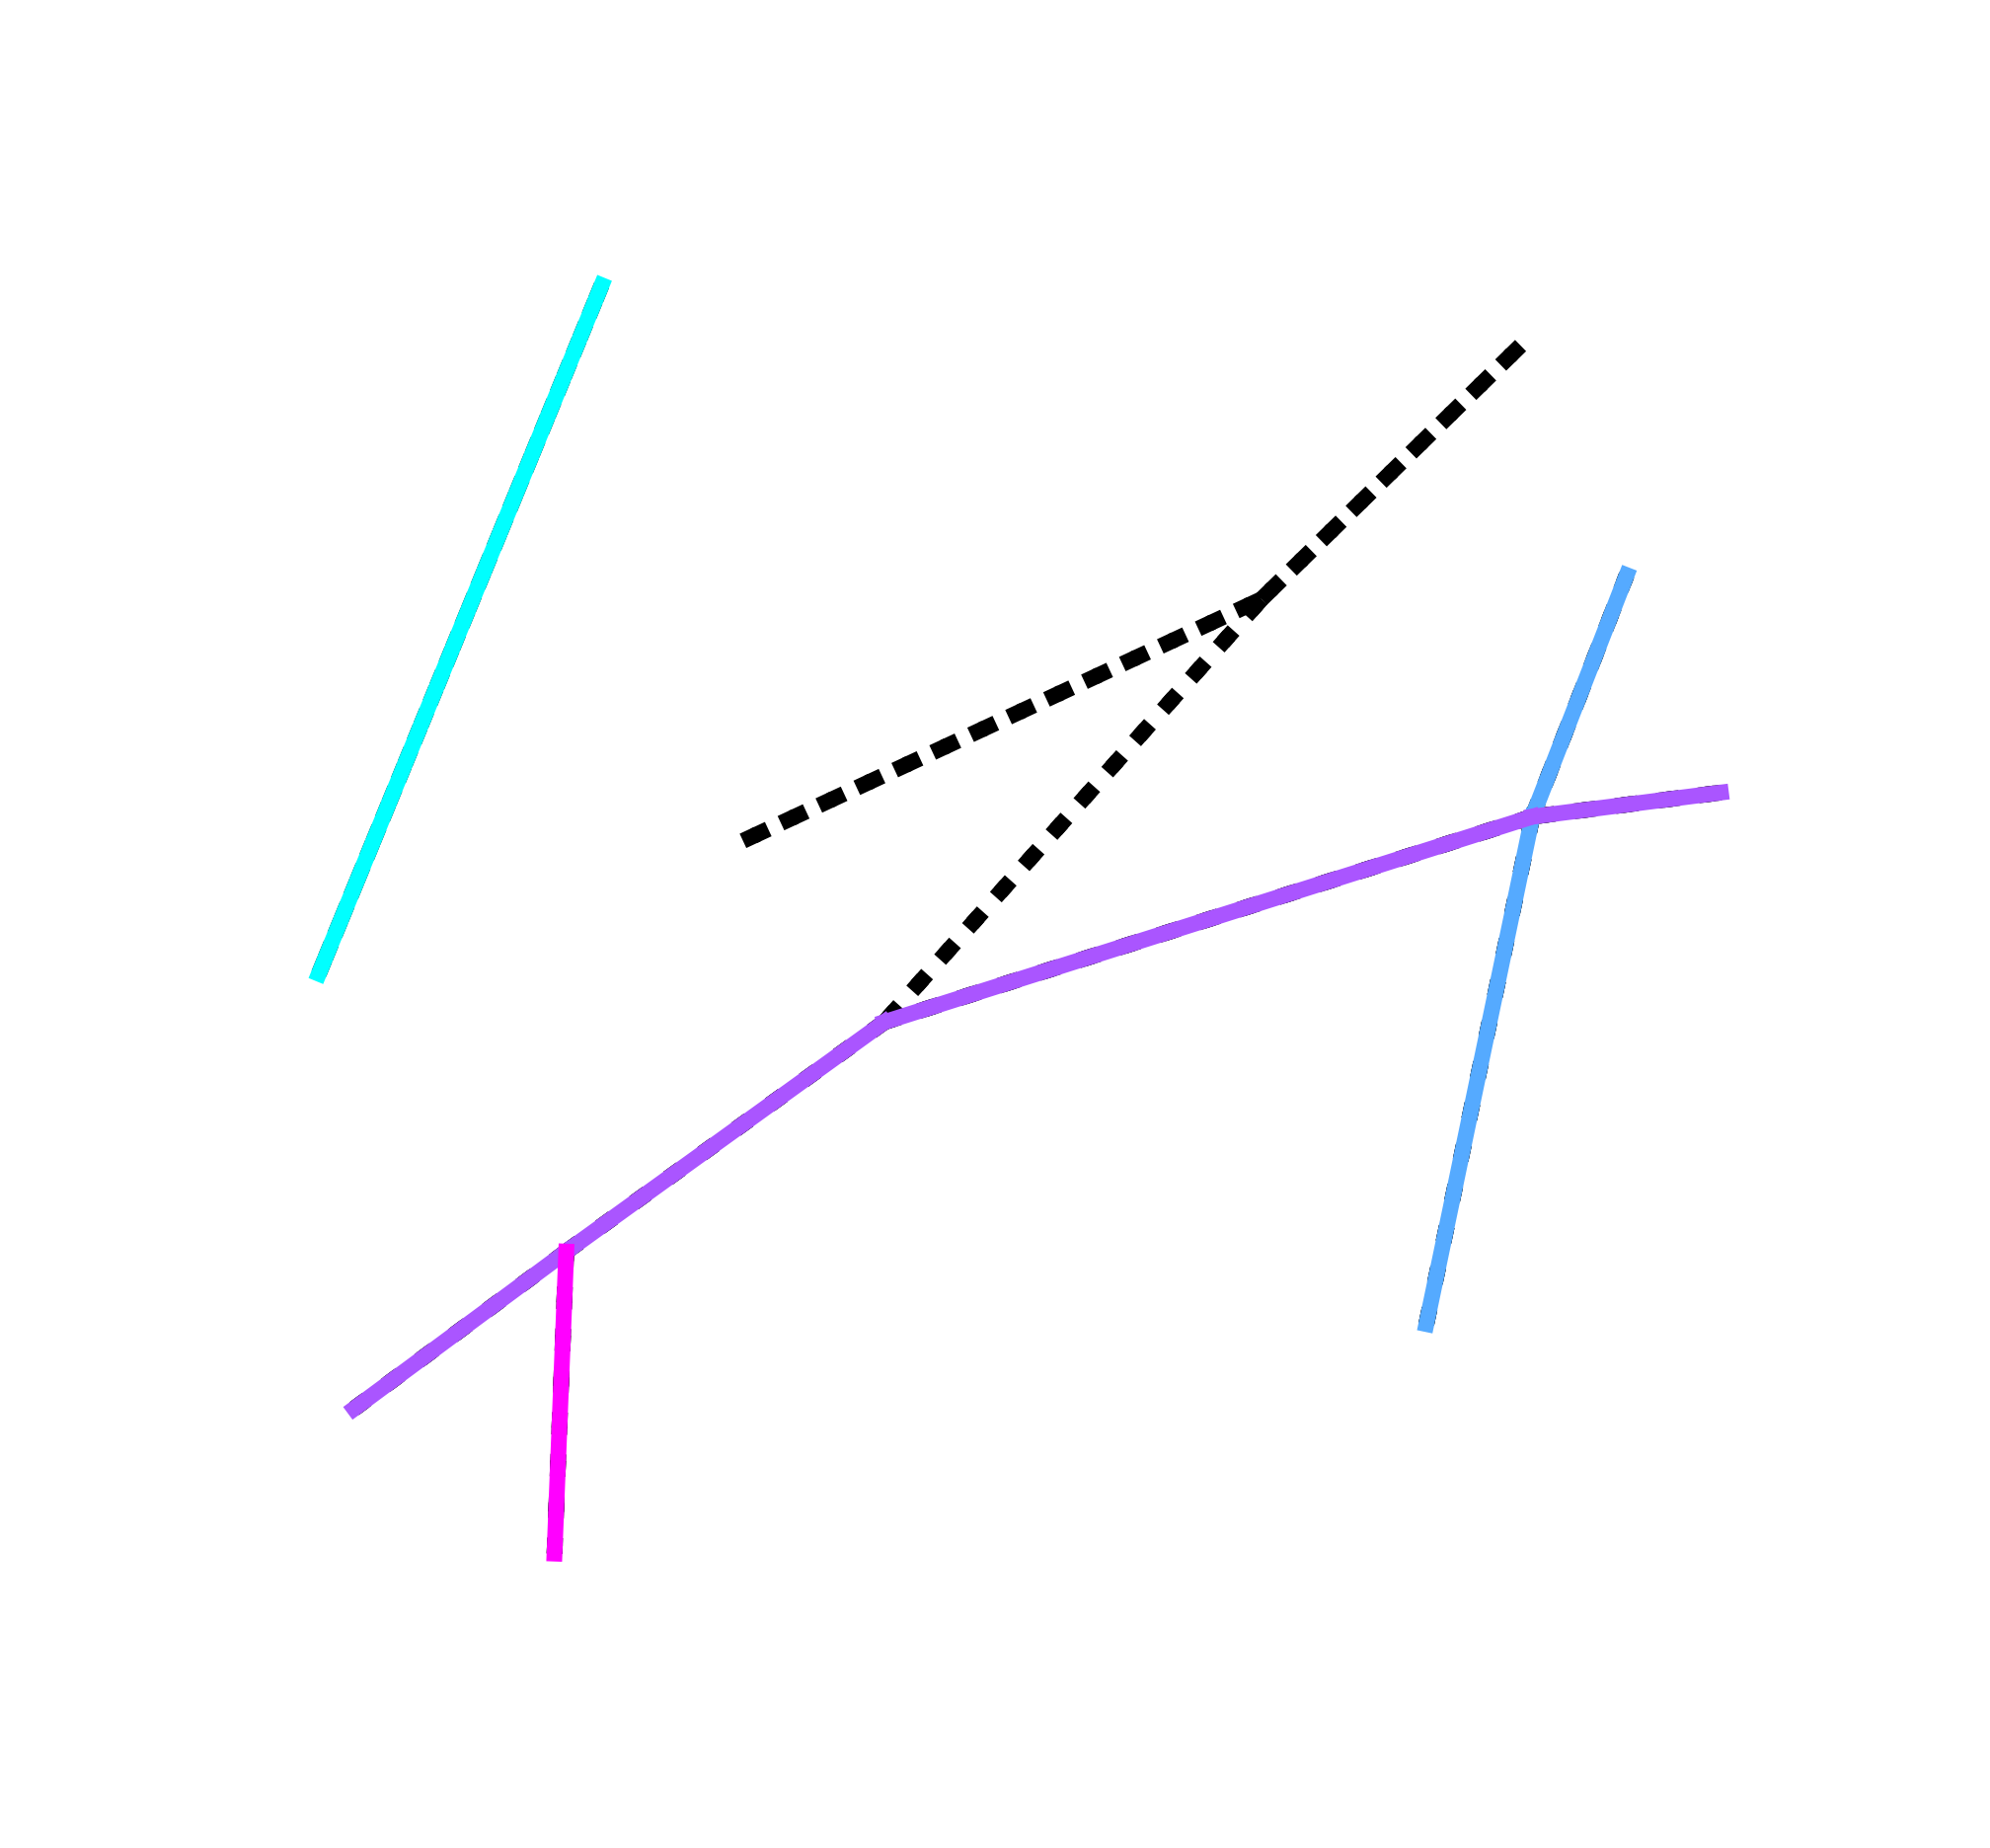
\includegraphics[height=1.5in]{resultImages/QFS7-DeFiNeExactMatch-30.png}
        \caption{Representaci\'on del resultado de DeFiNe con \'angulo de 30\textdegree, con 4 filamentos correctamente individualizados, identificados con colores.}
        \label{fig:SpinningMarchantiaResults-define30Exact}
    \end{subfigure}
    \begin{subfigure}[t]{0.48\textwidth}
        \centering
        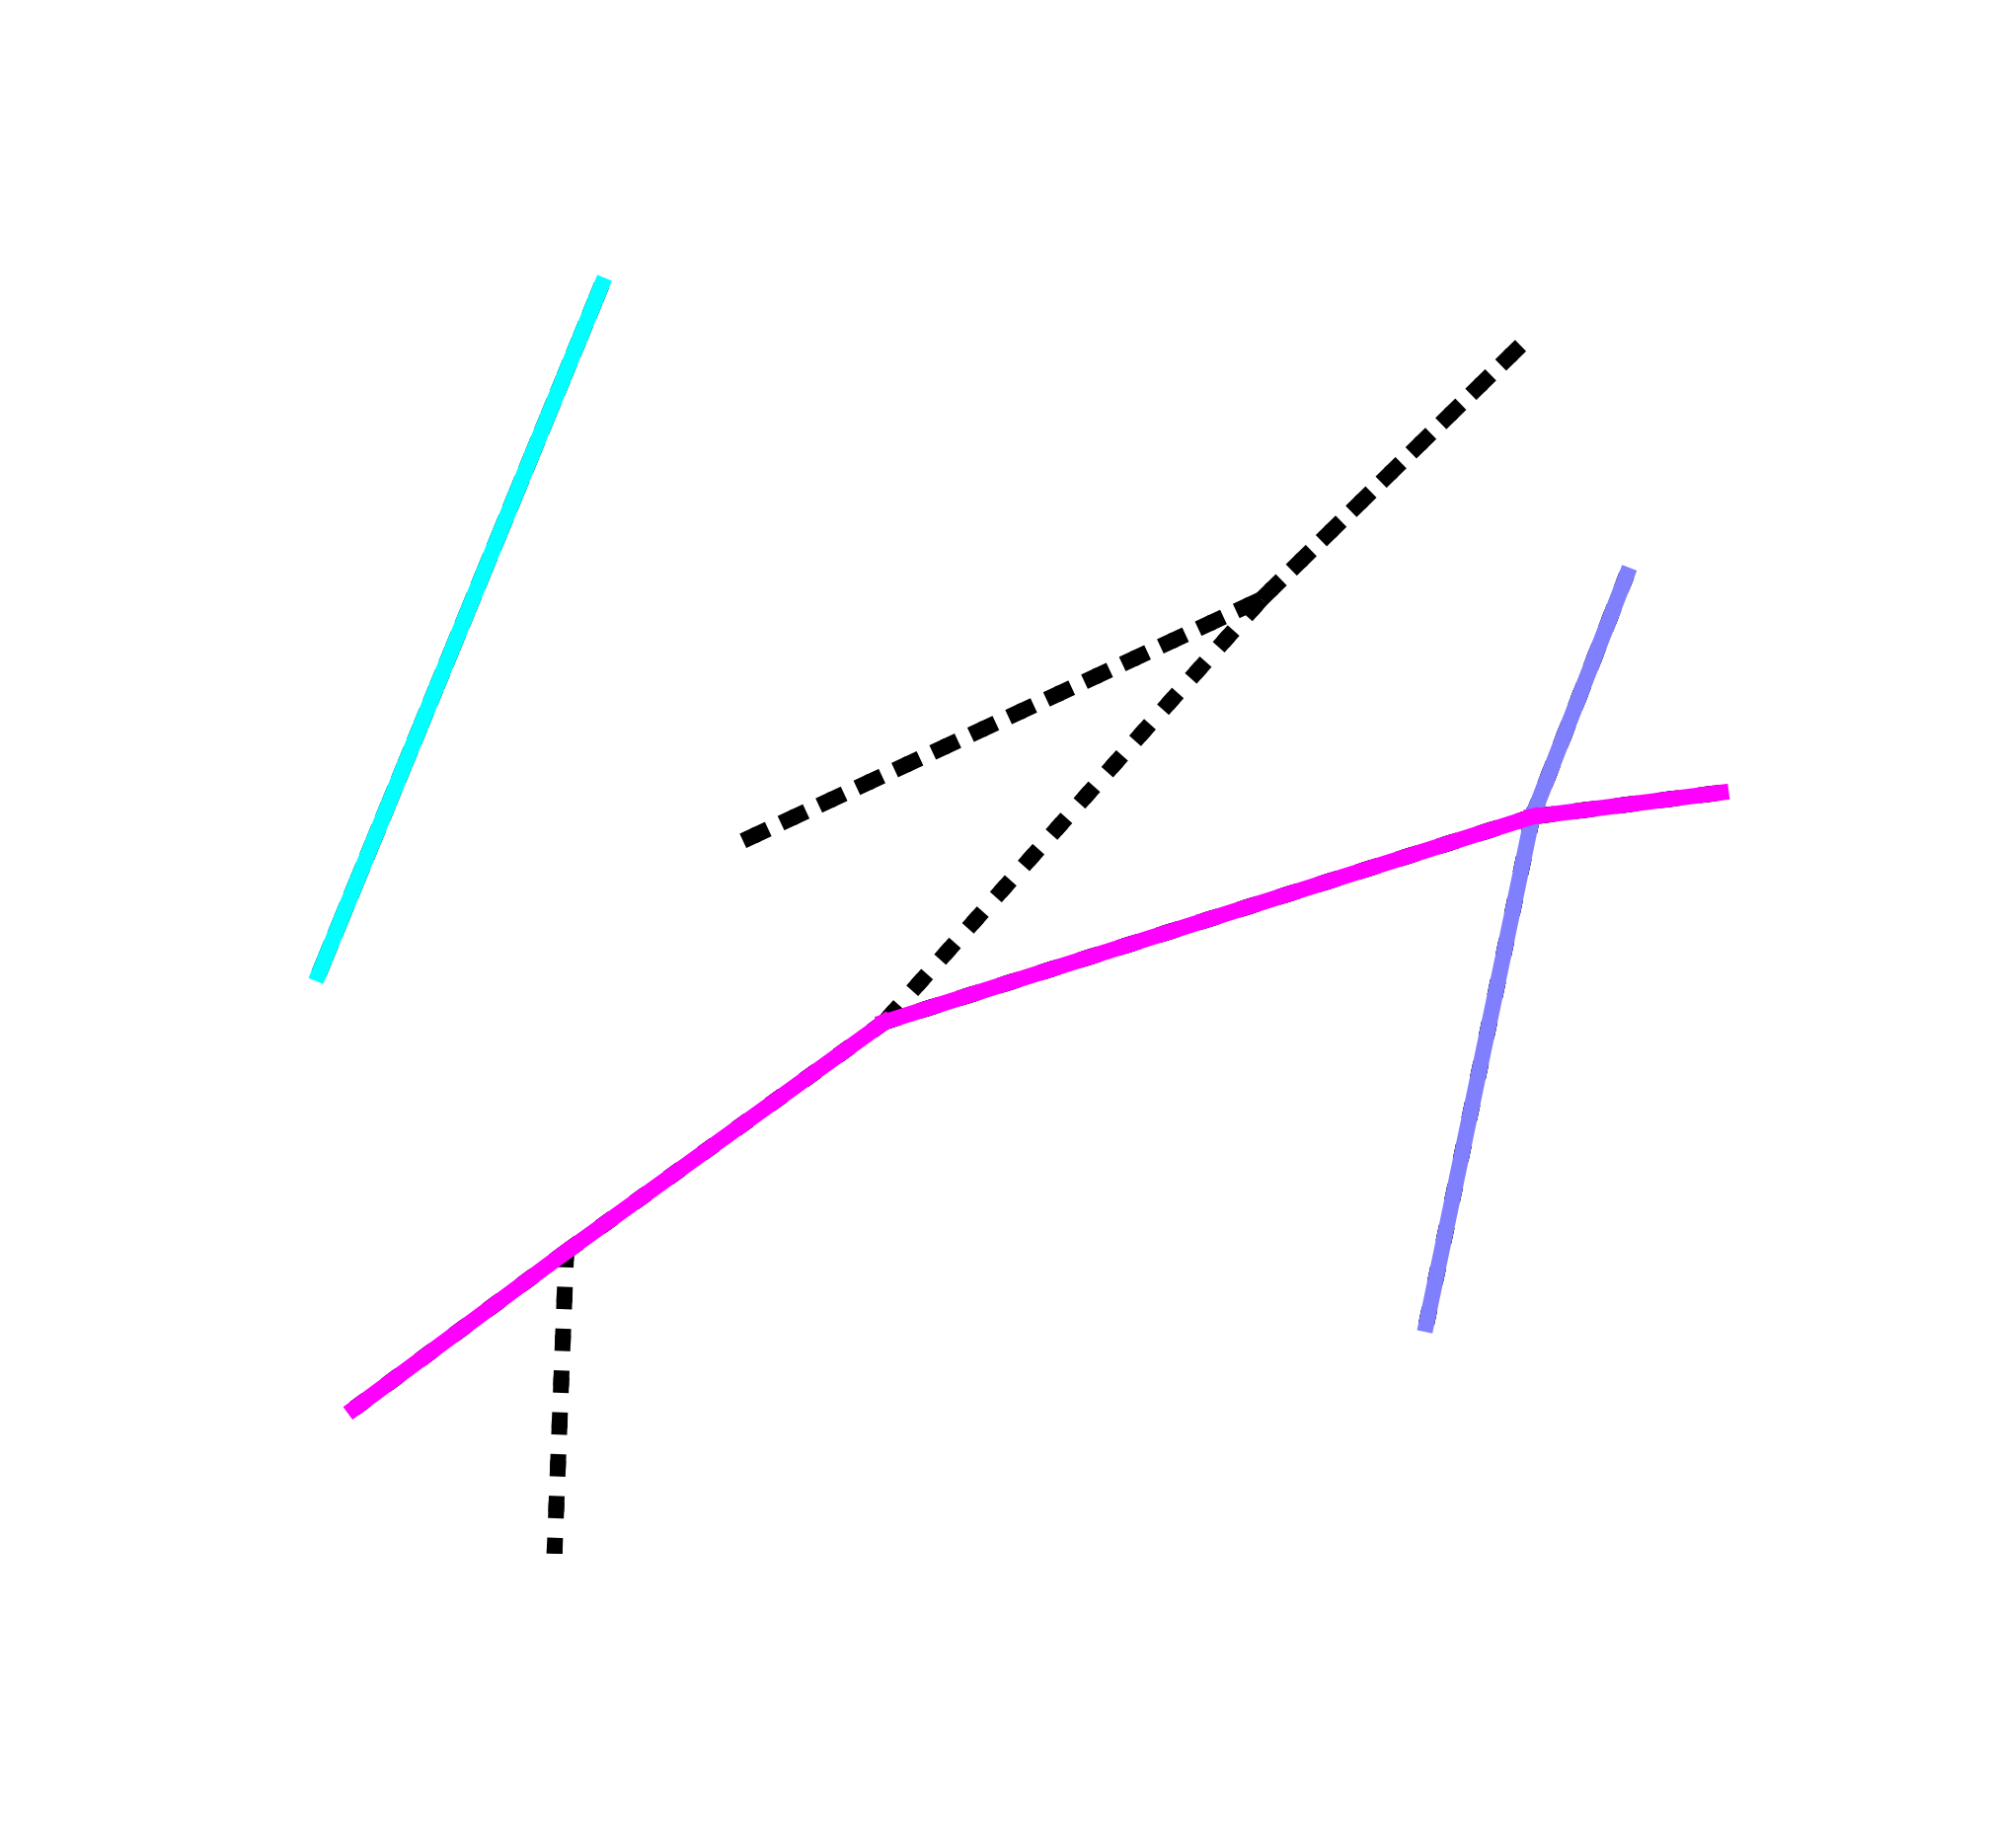
\includegraphics[height=1.5in]{resultImages/QFS7-DeFiNeExactMatch-60.png}
        \caption{Representaci\'on del resultado de DeFiNe con \'angulo de 60\textdegree, con 3 filamentos correctamente individualizados, identificados con colores.}
        \label{fig:SpinningMarchantiaResults-define60Exact}
    \end{subfigure}
    \vskip\baselineskip
    \begin{subfigure}[t]{0.47\textwidth}
        \centering
        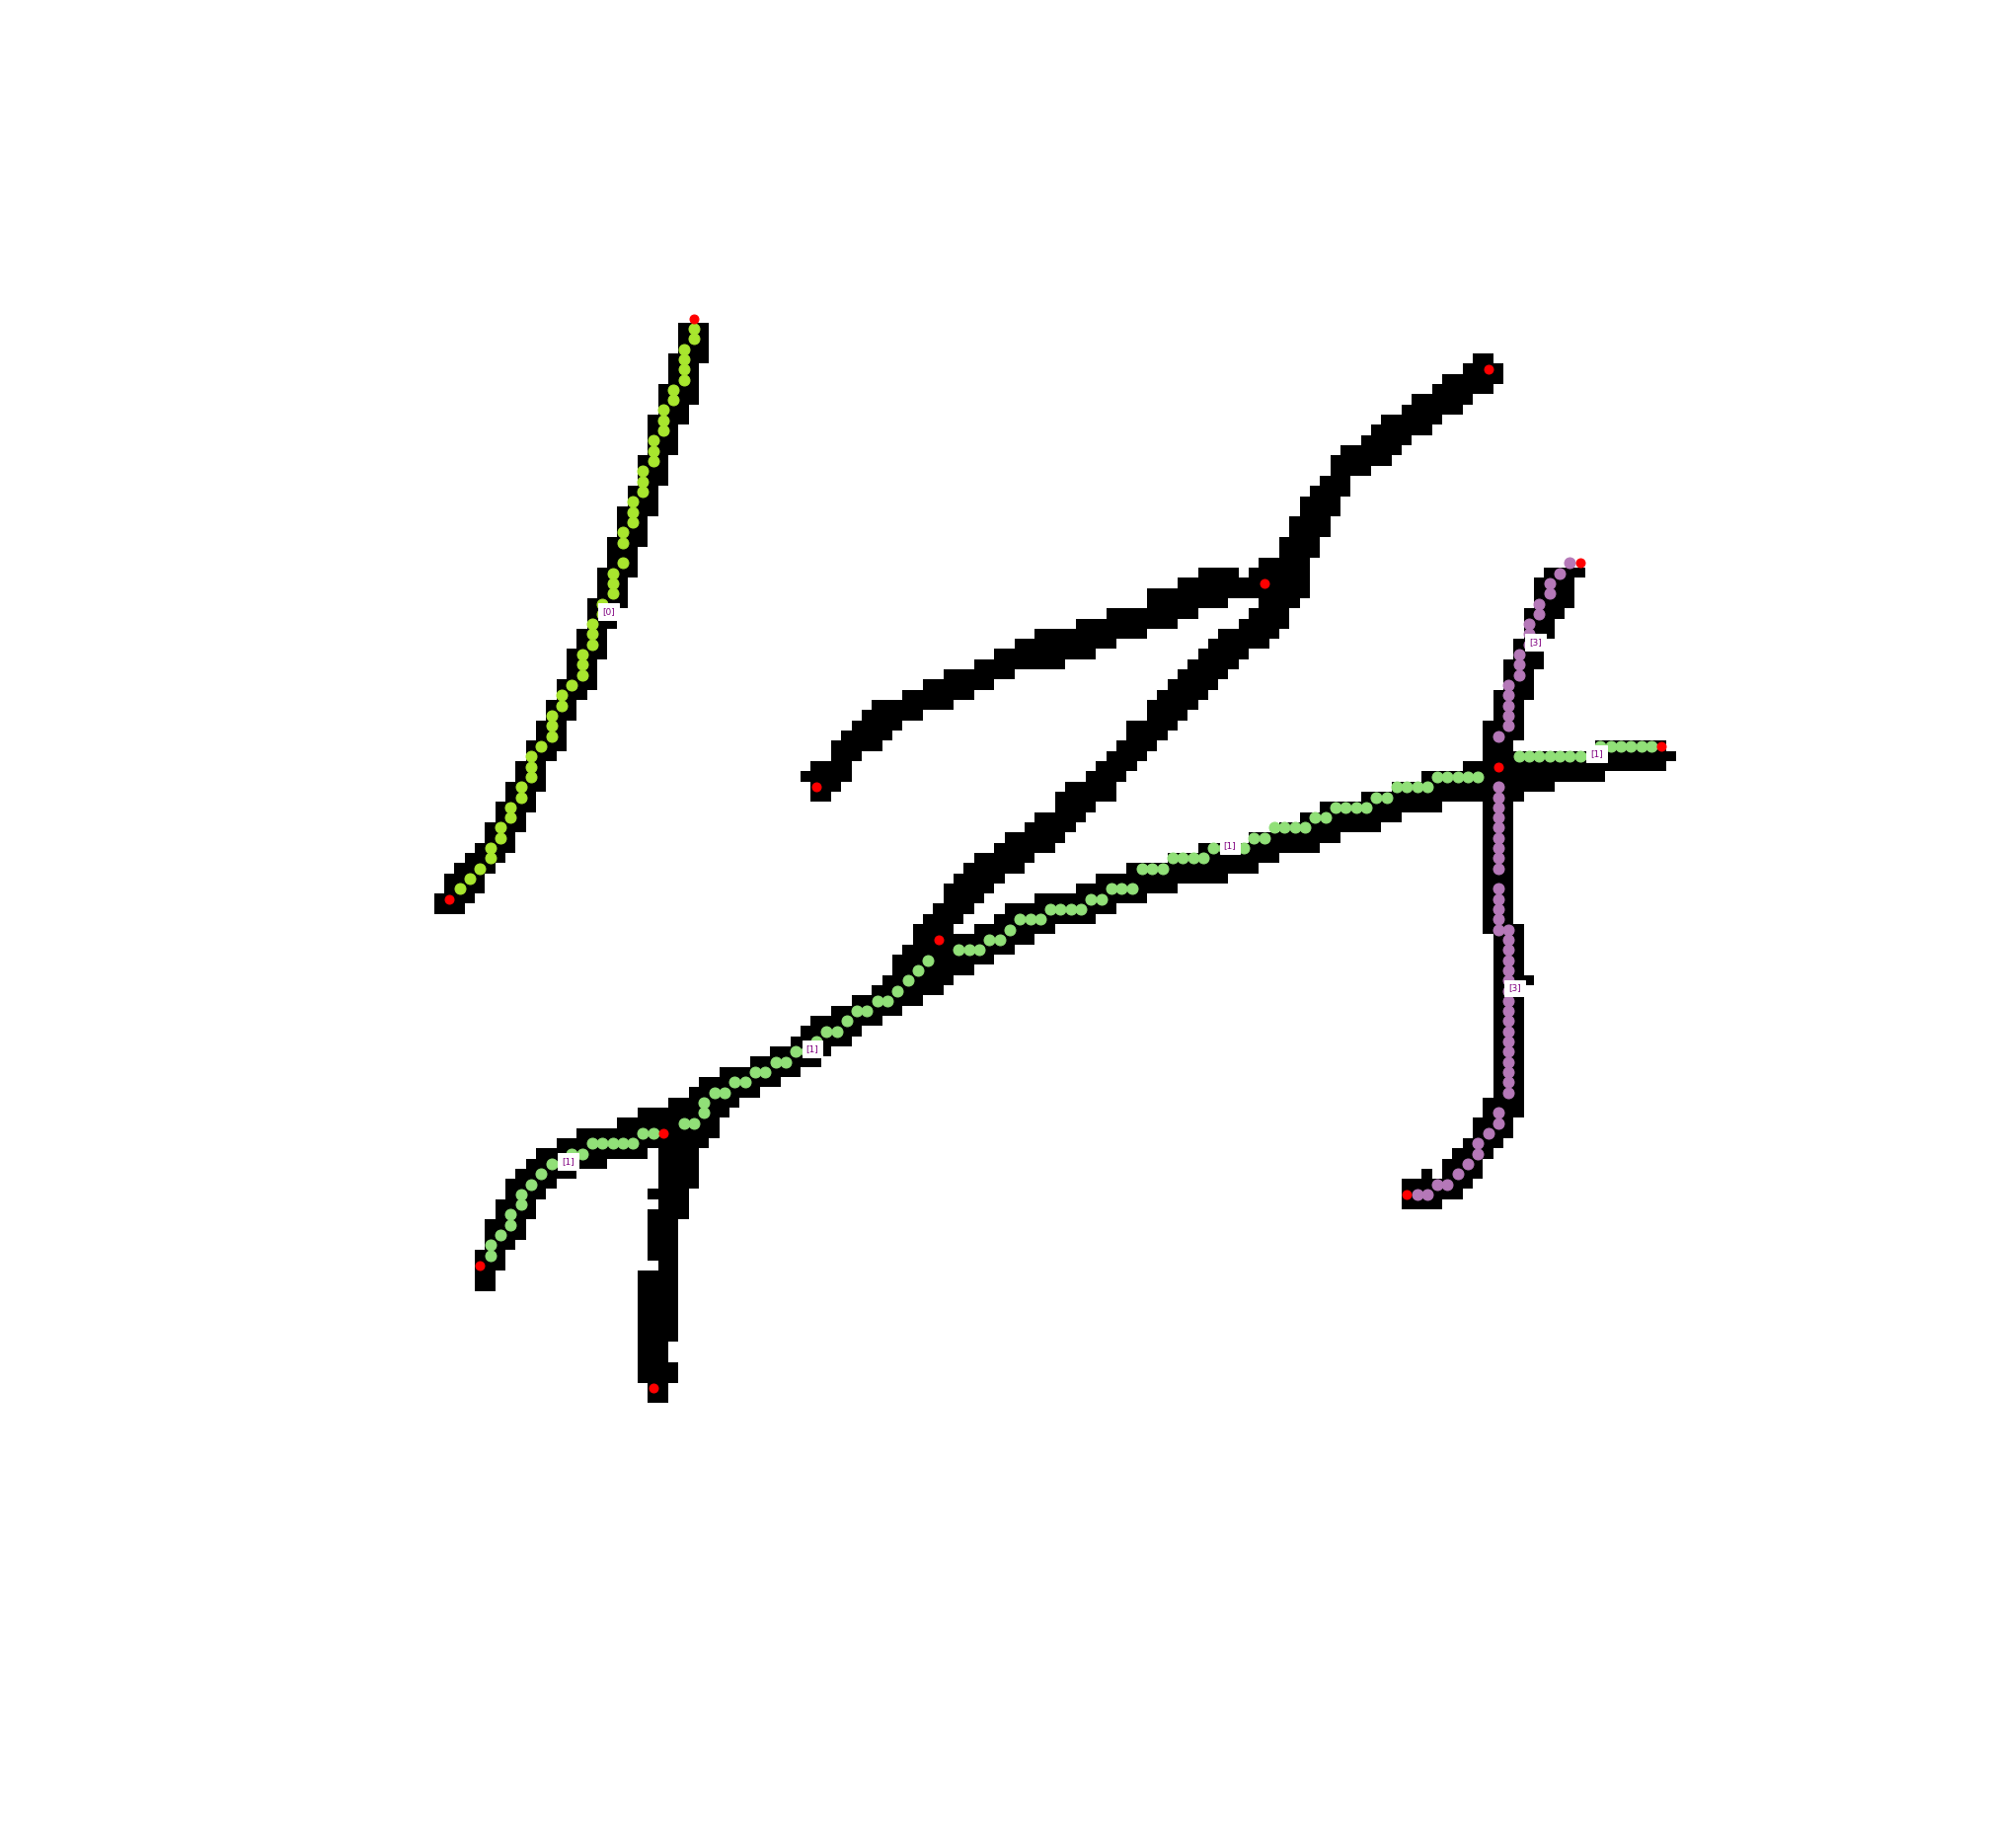
\includegraphics[scale=0.13]{resultImages/Synth-QuantitativeIFS-Fig7-phil-s1271-v05-exactMatch-antLabeled.png}
        \caption{Filamentos individualizados con colores a partir de la mejor iteraci\'on del algoritmo propuesto con la configuraci\'on definida como Modo 1.}
        \label{fig:SynthQFS7-Individualizacion-BestP1}
    \end{subfigure}
    \hspace{0.2cm}
    \begin{subfigure}[t]{0.47\textwidth}
        \centering
        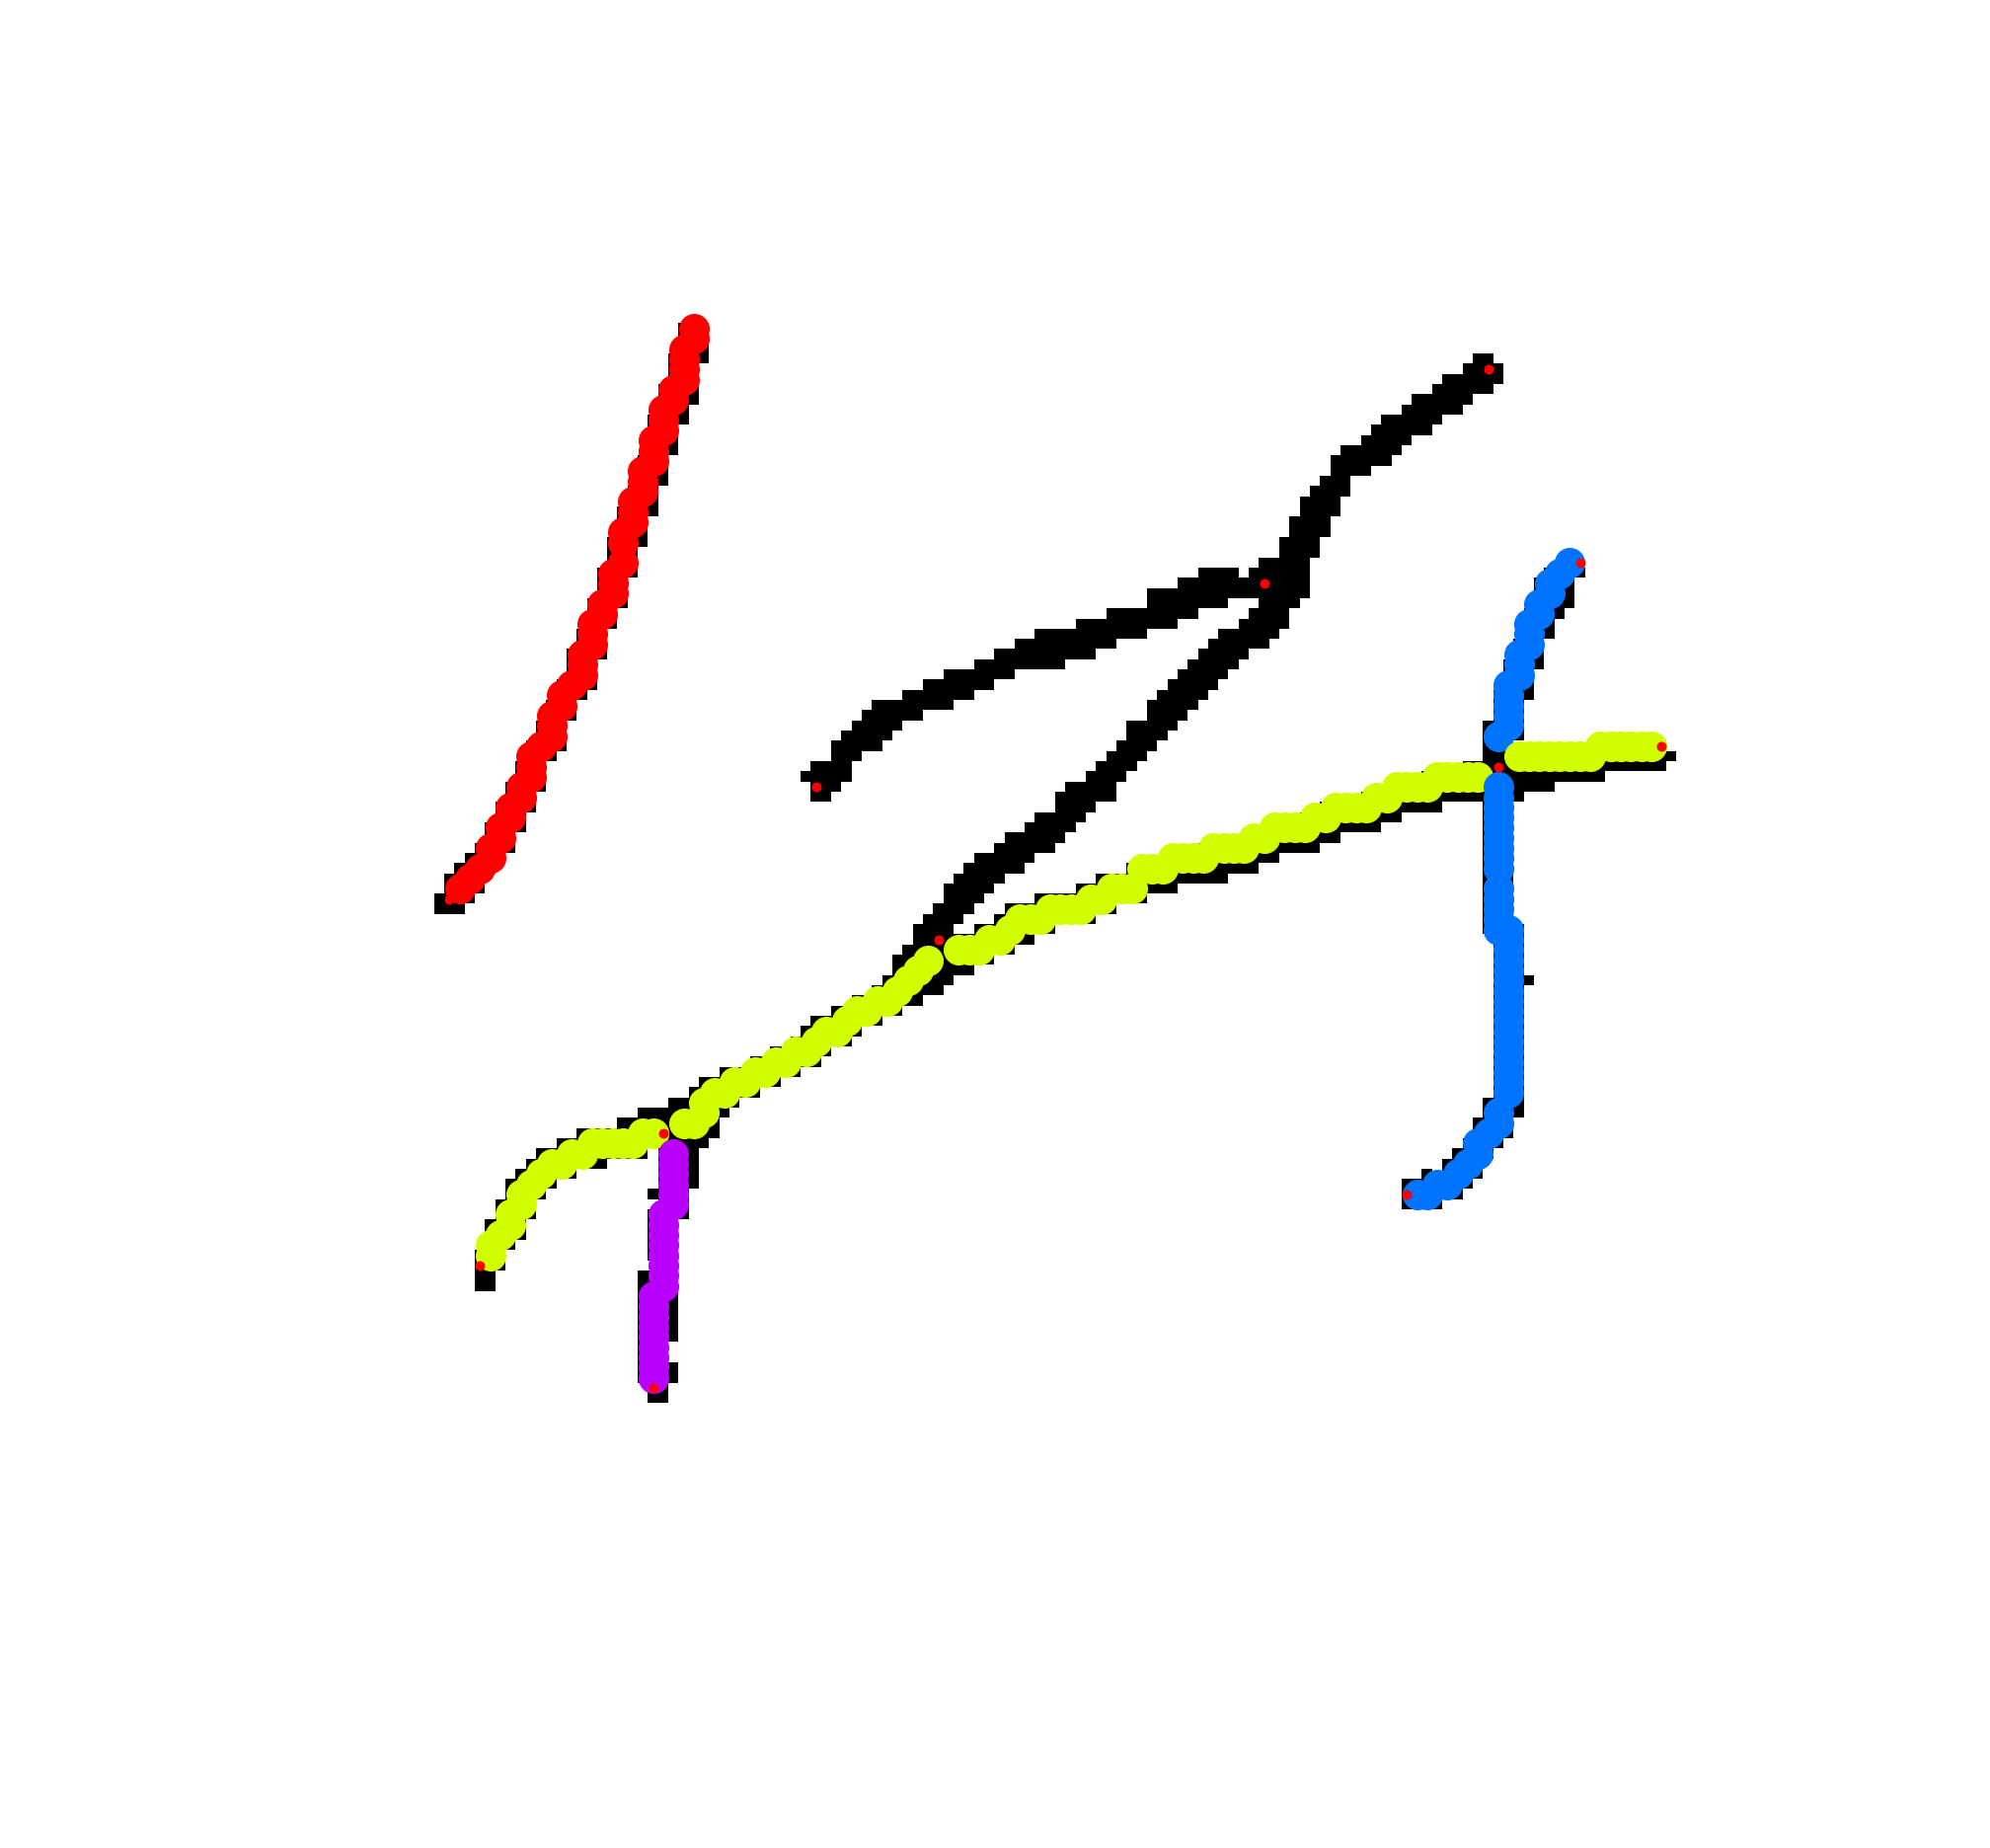
\includegraphics[scale=0.13]{resultImages/Synth-QuantitativeIFS-Fig7-phil-s1271-v056-exactMatch-antLabeled.png}
        \caption{Filamentos individualizados con colores a partir de la mejor iteraci\'on del algoritmo propuesto con la configuraci\'on definida como Modo 2.}
        \label{fig:SynthQFS7-Individualizacion-BestP2}
    \end{subfigure}
        
    \caption{Individualizaci\'on de filamentos correctos respecto a la evaluaci\'on de un experto para la Figura \ref{fig:synth-QFS-7}. El algoritmo propuesto individualiza correctamente 3 filamentos con la configuraci\'on para microt\'ubulos de planta, mejorando a 4 filamentos con una configuraci\'on m\'as simple.}
    \label{fig:Synth-QIFS-Result}
\end{figure*}

%\clearpage
%\newpage
%%%%%%%%%% End synth QFS 7 - Begin Synth DeFiNe 1b %%%%%%%



%Resultados Synth Define

Como se menciona en la secci\'on \ref{sec:graphImageExtraction}, la Figura \ref{fig:synth-Define-1b} corresponde a una parte de la Figura 1b en \cite{breuer2015define}, siendo la \'unica imagen para la que se dispone de un grafo ponderado seg\'un el criterio de los autores de DeFiNe. As\'i, se asume que aquel es el resultado \'optimo, en el que se individualizan correctamente los 5 filamentos. Una diferencia del grafo utilizado en la evaluaci\'on del algoritmo propuesto, con respecto al grafo que permite individualizar aquellos 5 filamentos, radica en que el utilizado con el algoritmo propuesto divide 1 de los 5 filamentos en 2, generando 6 filamentos en total. Es por ello, que las dem\'as evaluaciones con respecto a la Figura \ref{fig:synth-Define-1b} indican 6 filamentos como {\it ground truth}.


En la evaluaci\'on del algoritmo propuesto utilizando los par\'ametros definidos para microt\'ubulos de plantas, se obtienen 3 individualizaciones correctas de los 5 filamentos que corresponden al {\it ground truth}. En esta evaluaci\'on, denominada Modo 3, s\'olo 1 filamento individualizado se encuentra dentro del grupo de filamentos que se intersectan y sobreponen entre s\'i. Es posible atribuir esto a la curvatura de algunos de los filamentos sint\'eticos, la que es mayor a la que se espera de un microt\'ubulos de planta. Para complementar la evaluaci\'on, se realiza una evaluaci\'on definida como Modo 4 en la que se elige el tipo de c\'elula sint\'etica, modificando el factor $Max\_Axial\_Displacement$ a 2, asociado a la curvatura que presenta la figura, y no utilizando la heur\'istica de asignaci\'on inicial completa, dado que no existen casos complejos de nacimiento de filamentos a partir de otros como en filamentos reales.

As\'i, en la evaluaci\'on Modo 4 se encuentra un filamento adicional, y a su vez, es capaz de encontrar el filamento naranja de la individualizaci\'on manual del experto, indicado en la Figura \ref{fig:synth-Define-1b-graph-gt}, pero es descartado por no respetar el criterio de la magnitud de desplazamiento entre segmentos. El comportamiento del filamento naranja en el {\it ground truth} realiza un cambio de sentido en sus curvaturas, adem\'as de que estas son bastante pronunciadas, lo que no es un comportamiento esperado en los filamentos estudiados durante esta investigaci\'on. Los resultados se presentan en la Tabla \ref{tab:synth-Define-1b}.


%Con respecto a las medidas, se obtiene un alto valor de VI, lo que es atribuible a que en este caso existen varios casos de solapamiento entre filamentos, mientras que con la configuraci\'on para microt\'ubulos de planta, los \'indices {\it Rand} y {\it Jaccard} son disimiles entre s\'i, con enf\'asis en que el \'indice {\it Jaccard} arroja un resultado muy cercano a 0.


\begin{table}[h]
    \centering
    \begin{tabular}{|c|c|c|c|c|c|c|c|c|c|c|c|}
    \hline
          Algoritmo & P & P* & R & R* & F1 & F1* & C/P & C/P* & C/GT & C/GT* & T[s] \\ \hline
         DeFiNe 30\textdegree  & 0.33 & - & 0.18 & - & 0.23 & - & 2/11 & - & 2/5 & - & 2.82 \\
         DeFiNe 60\textdegree & 0.23 & - & 0.25 & - & 0.24 & - & 2/7 &- & 2/5 & - & 3.65\\
        Modo 3 & 0.34 & 0.35 & 0.27 & 0.28 & 0.3 & 0.31 & 3/9.2 & 3/9 & 3/6 & 3/6 & 0.35\\
        %Mejor Iteraci\'on P1 & 0.5714 & 0.5714 & 0.5714 & 3/5 &  & 0.3135 \\
        Modo 4 & 0.32 & 0.33 & 0.25 & 0.31 & 0.28 & 0.32 & 4/8.6 & 4/9 & 4/6 & 4/6 & 0.32\\
        % {\bf Mejor Iteraci\'on P2} & 0.875 & 1 & 0.9333 & 4/5 & 4/6 & 0.3073\\
         \hline
    \end{tabular}
    \caption{Resultado de la individualizaci\'on de filamentos para la Figura \ref{fig:synth-Define-1b}. El valor m\'aximo de VI para este caso es 2.83321, dado que el grafo esta compuesto por 17 aristas. El n\'umero de filamentos definidos manualmente por un experto es 5. Las columnas P y R representan {\it Precision} y {\it Recall} respectivamente, la columna C/P refleja el n\'umero de filamentos correctos con respecto a los propuestos por cada m\'etodo, mientras que la columna C/GT indica la relaci\'on entre los filamentos correctamente individualizados por el m\'etodo y el criterio del experto. Finalmente la columna T indica el tiempo de ejecuci\'on. Las columnas sin asterisco representan el promedio de las iteraciones del algoritmo propuesto, mientras que las dem\'as indican el resultado de la mejor de las 5 iteraciones. Dado que DeFiNe es ejecutado una sola vez con cada \'angulo, su valor se muestra en las columnas promedio. La diferencia del n\'umero de filamentos en el {\it ground truth} se debe a que la herramienta utilizada para la obtenci\'on del grafo corta un filamento, generando un filamento adicional.}
    \label{tab:synth-Define-1b}
\end{table}

\begin{figure*}[h!]
    \centering
    \begin{subfigure}[t]{0.49\textwidth}
        \centering
        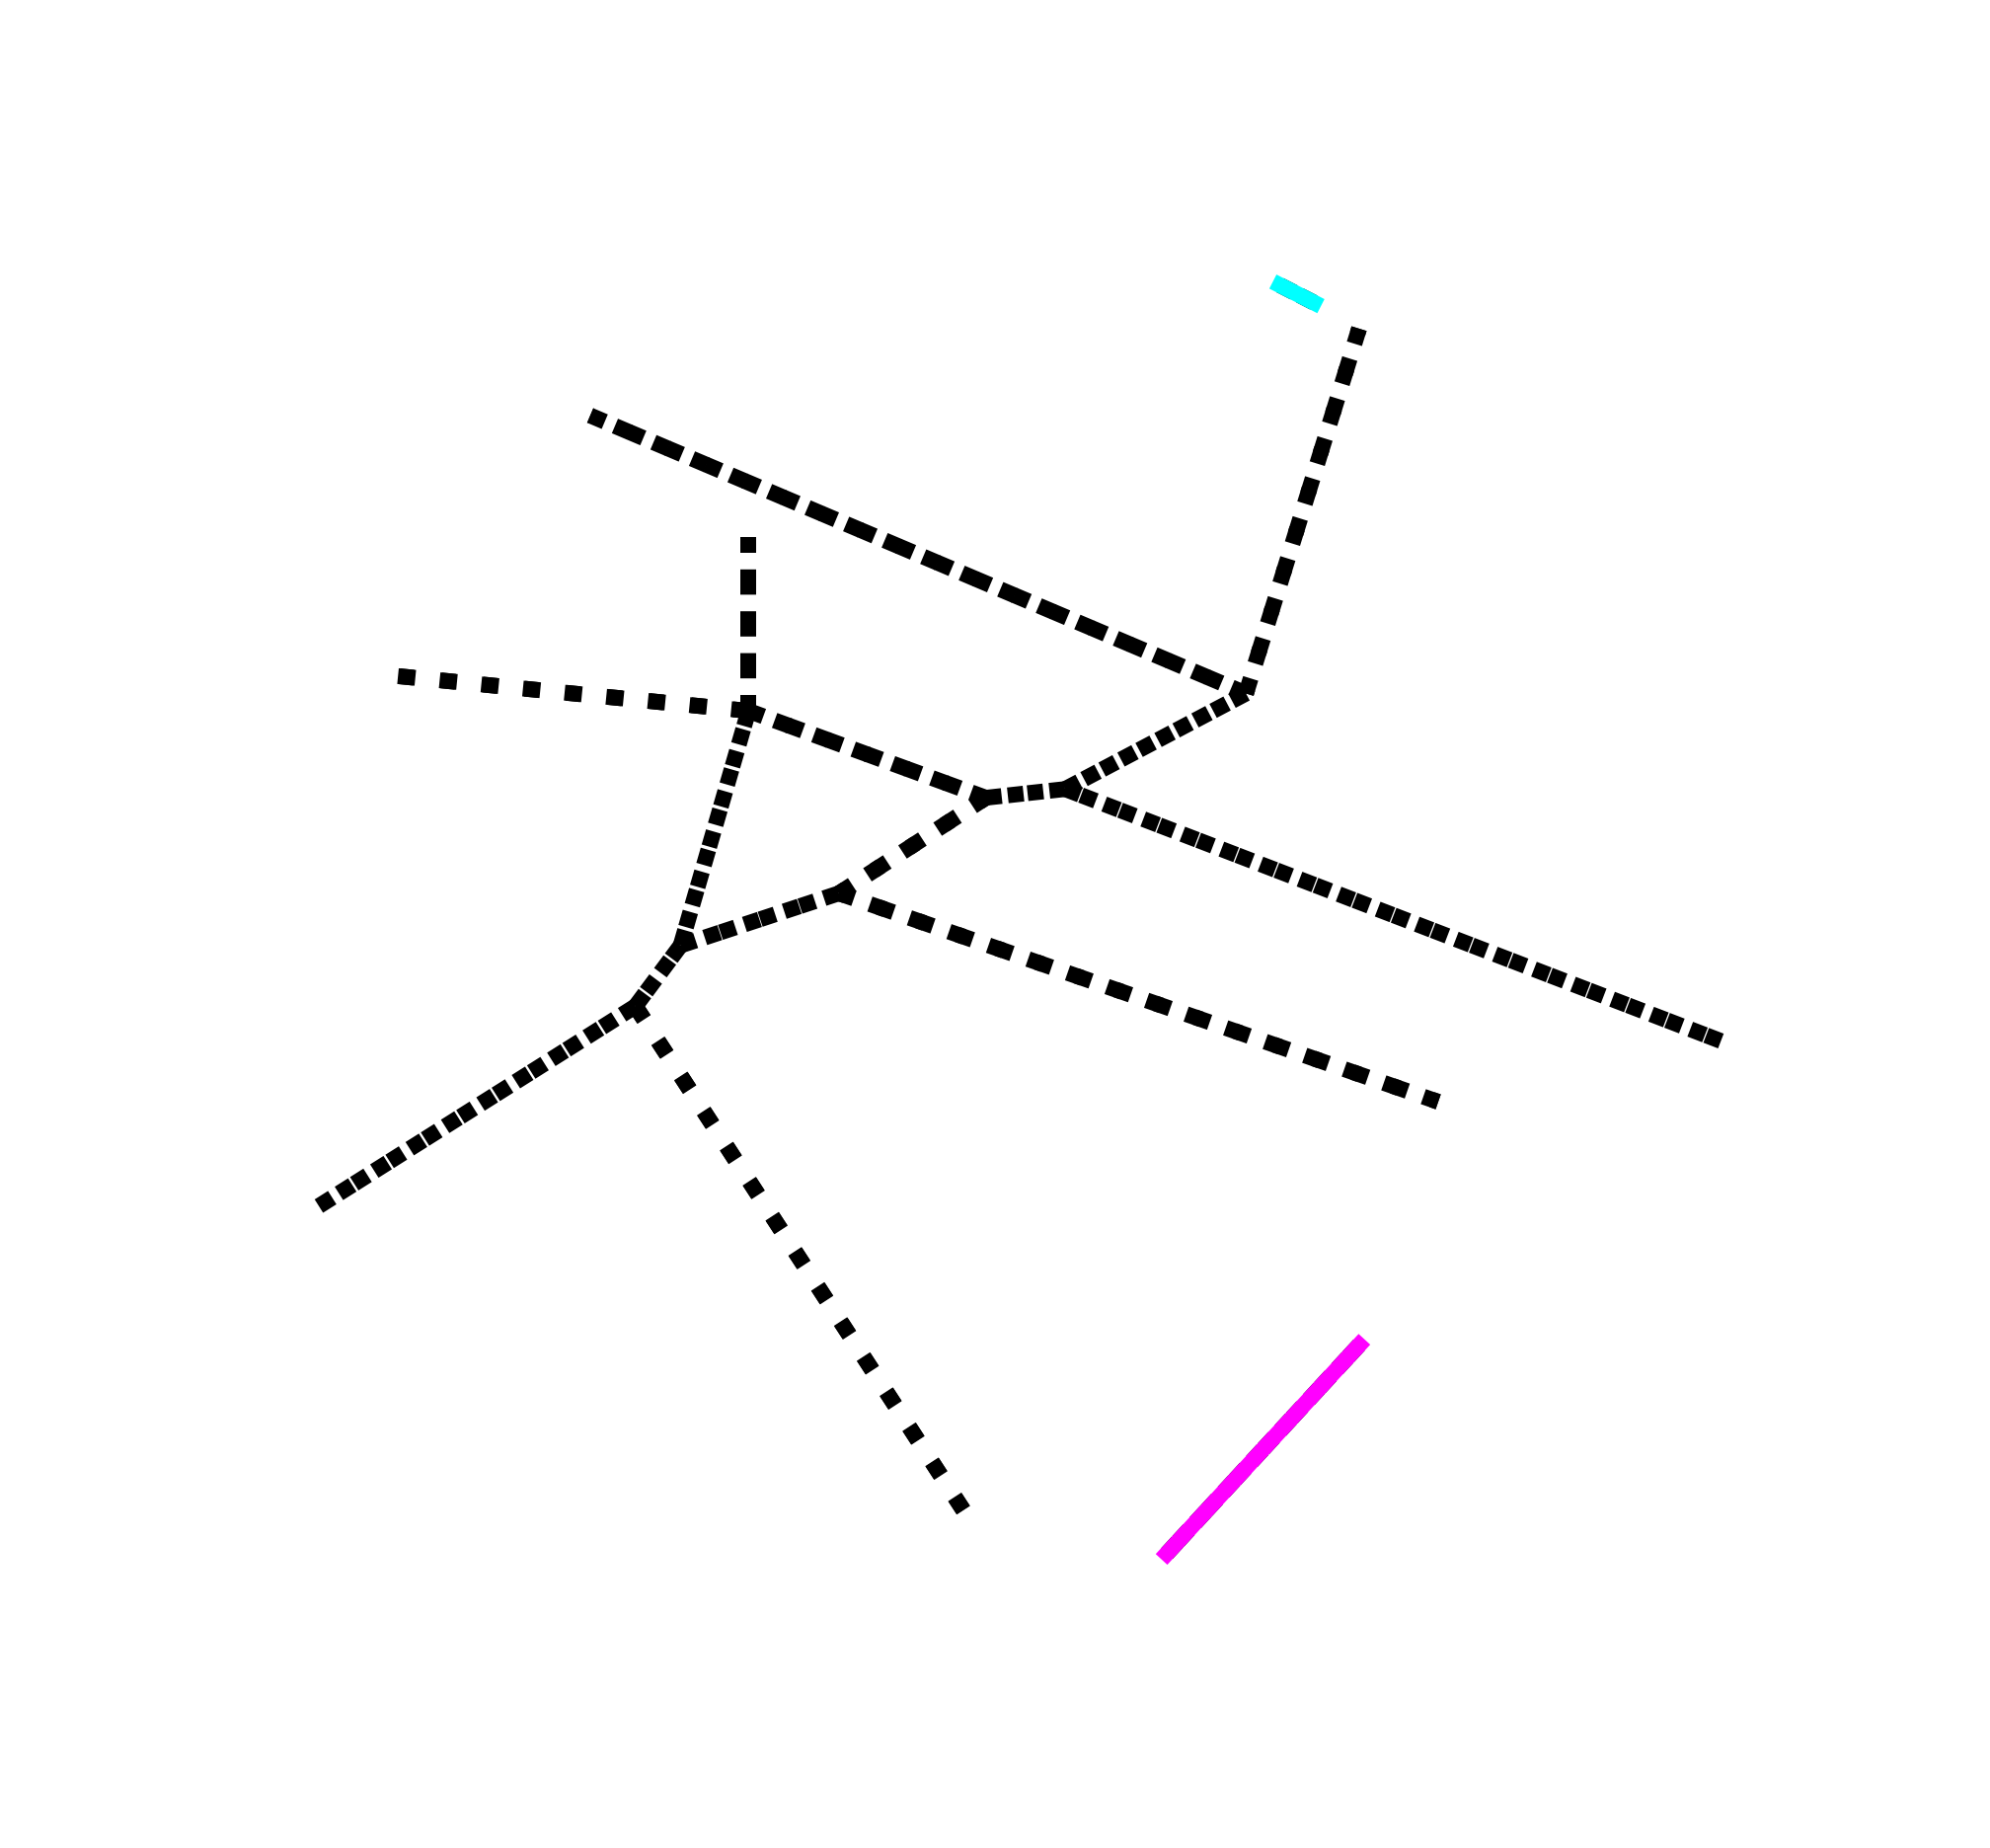
\includegraphics[scale=0.1]{resultImages/defineFig1b-DeFiNeExactMatch-30.png}
        \caption{Representaci\'on del resultado obtenido a trav\'es de DeFiNe con 30\textdegree, logrando 2 filamentos correctamente individualizados, identificados con colores.}
        \label{fig:SynthDefine-Results-define30Exact}
    \end{subfigure}
    ~
    \begin{subfigure}[t]{0.49\textwidth}
        \centering
        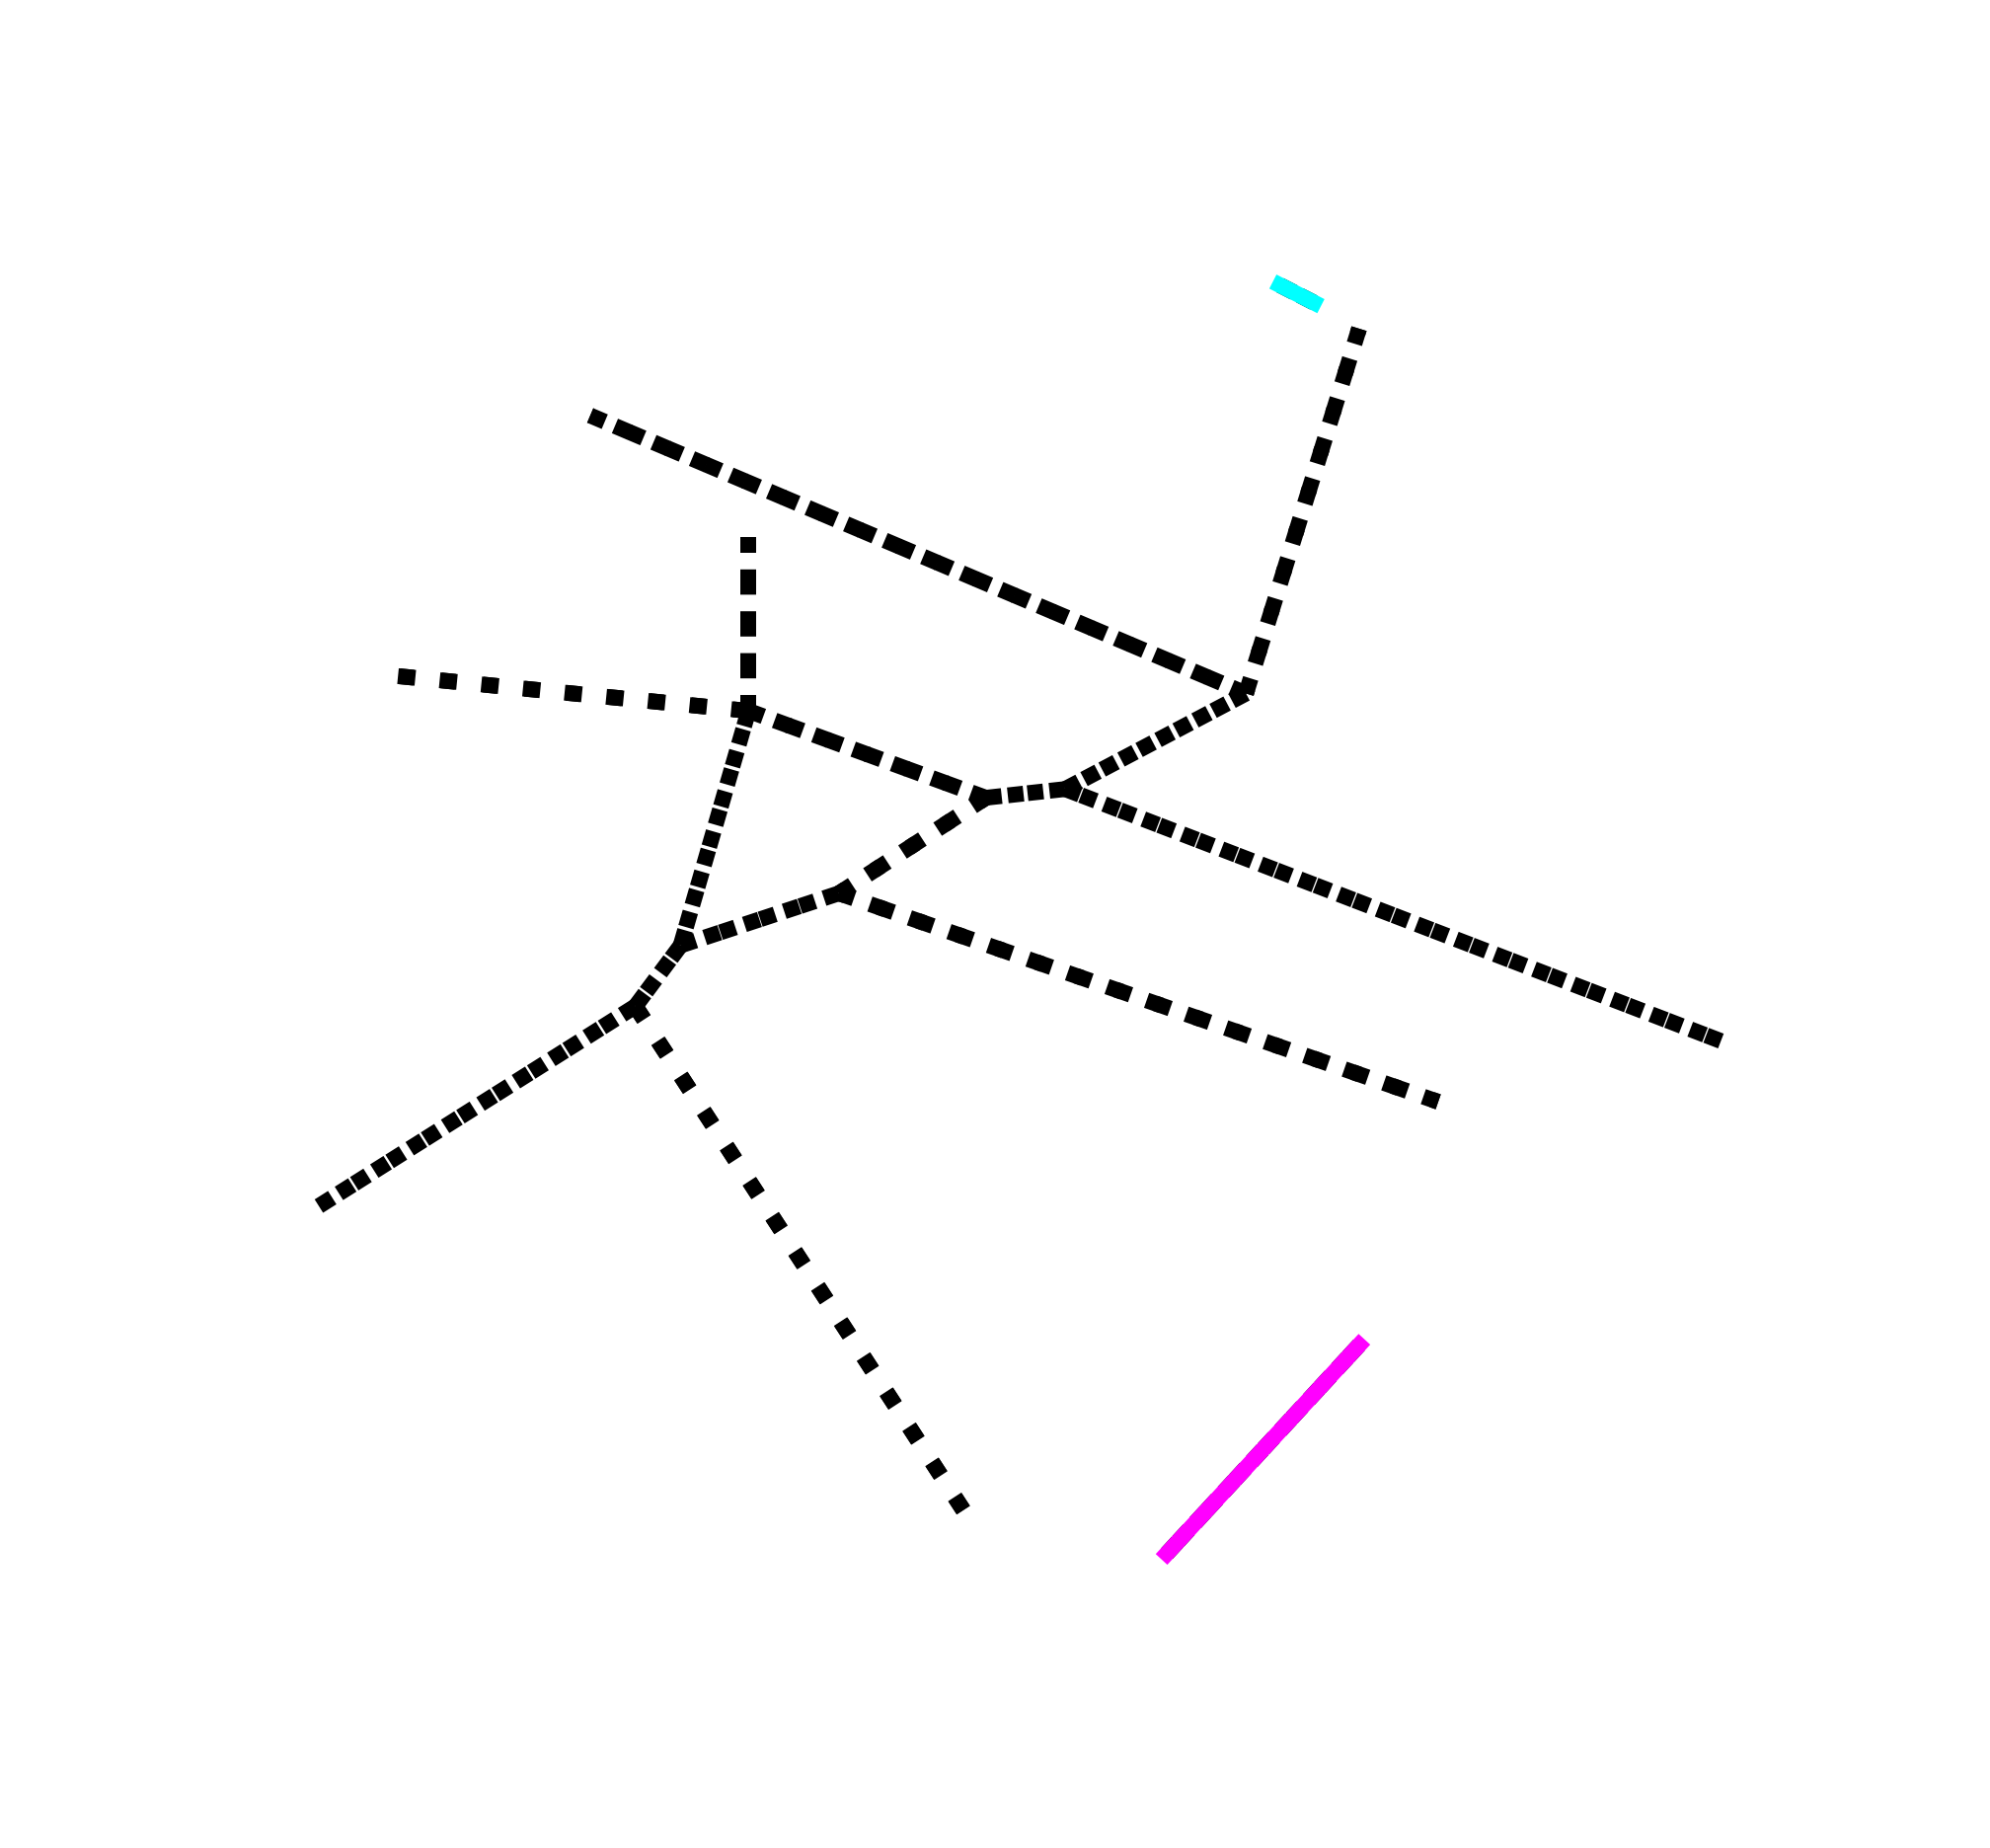
\includegraphics[scale=0.1]{resultImages/defineFig1b-DeFiNeExactMatch-60.png}
        \caption{Representaci\'on del resultado obtenido a trav\'es de DeFiNe con 60\textdegree, logrando 2 filamentos correctamente individualizados, identificados con colores.}
        \label{fig:SynthDefine-Results-define60Exact}
    \end{subfigure}
    \vskip\baselineskip
    
    \begin{subfigure}[t]{0.49\textwidth}
        \centering
        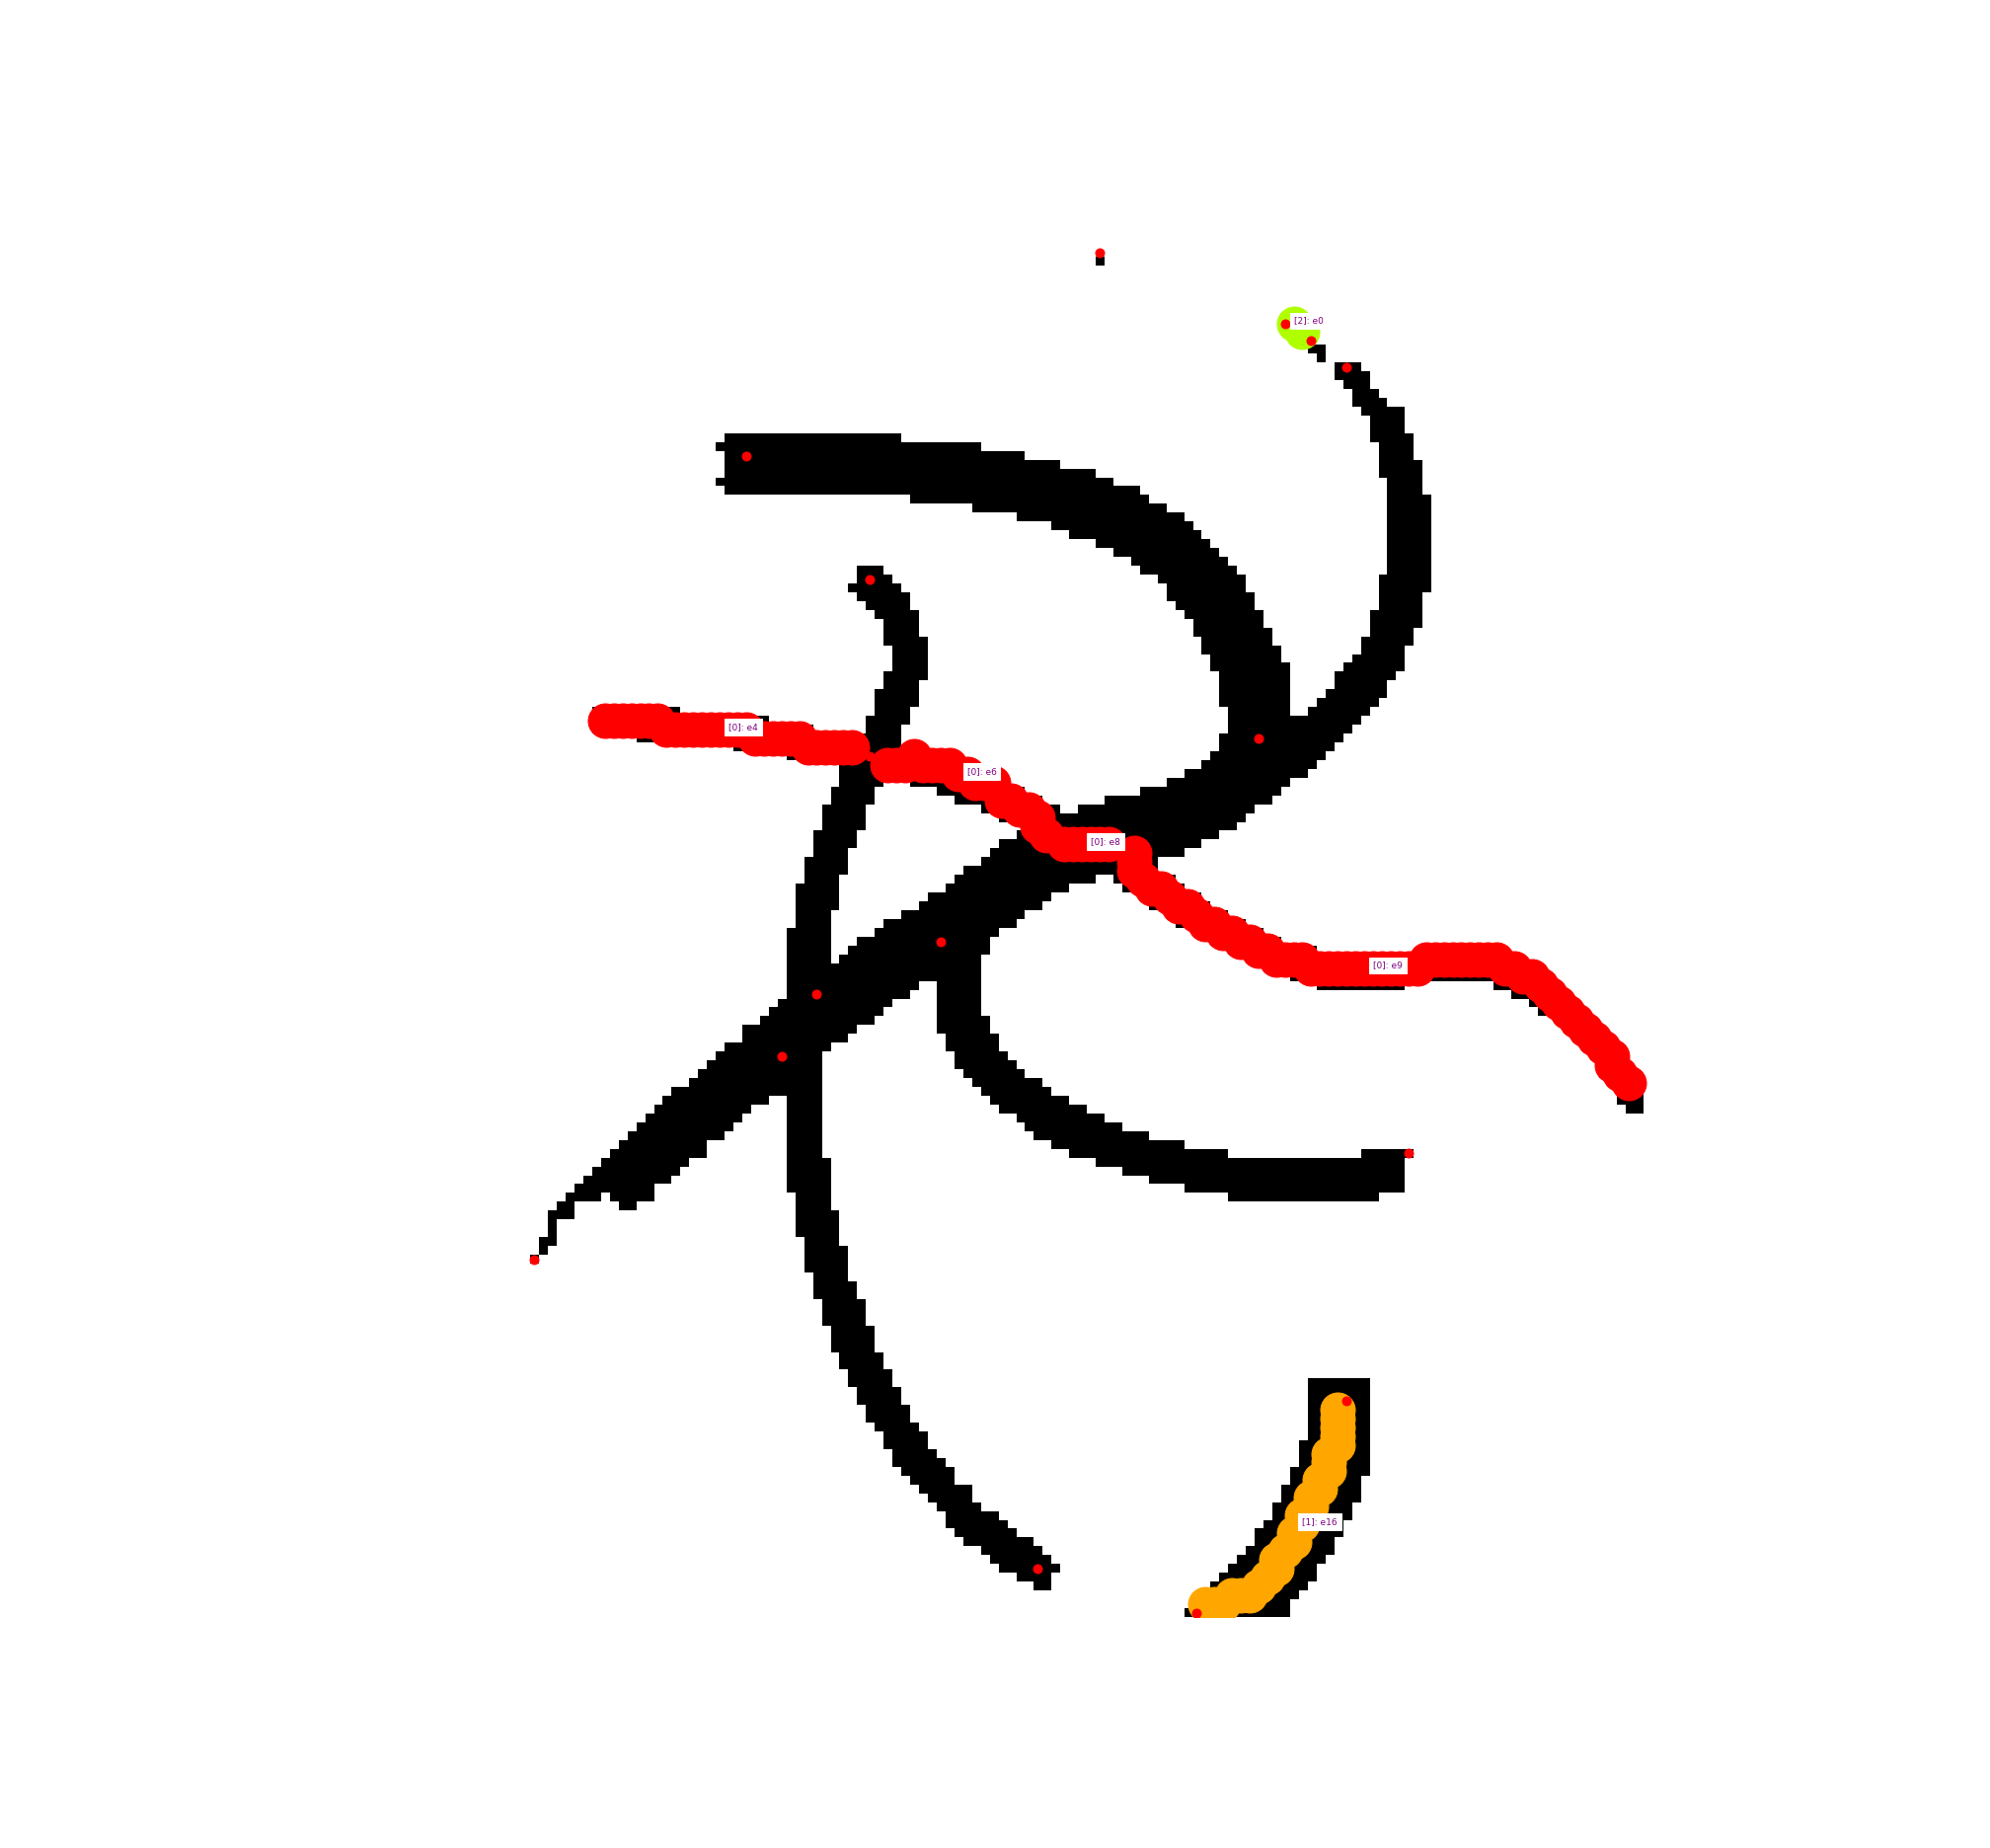
\includegraphics[scale=0.11]{resultImages/define-weighted-4-phil-s0-v05-exactMatch-antLabeled.png}
        \caption{3 filamentos correctamente individualizados por el algoritmo propuesto con la configuraci\'on definida como Modo 3.}
        \label{fig:SynthDefine-Individualizacion-BestP1}
    \end{subfigure}
    ~
    \begin{subfigure}[t]{0.49\textwidth}
        \centering
        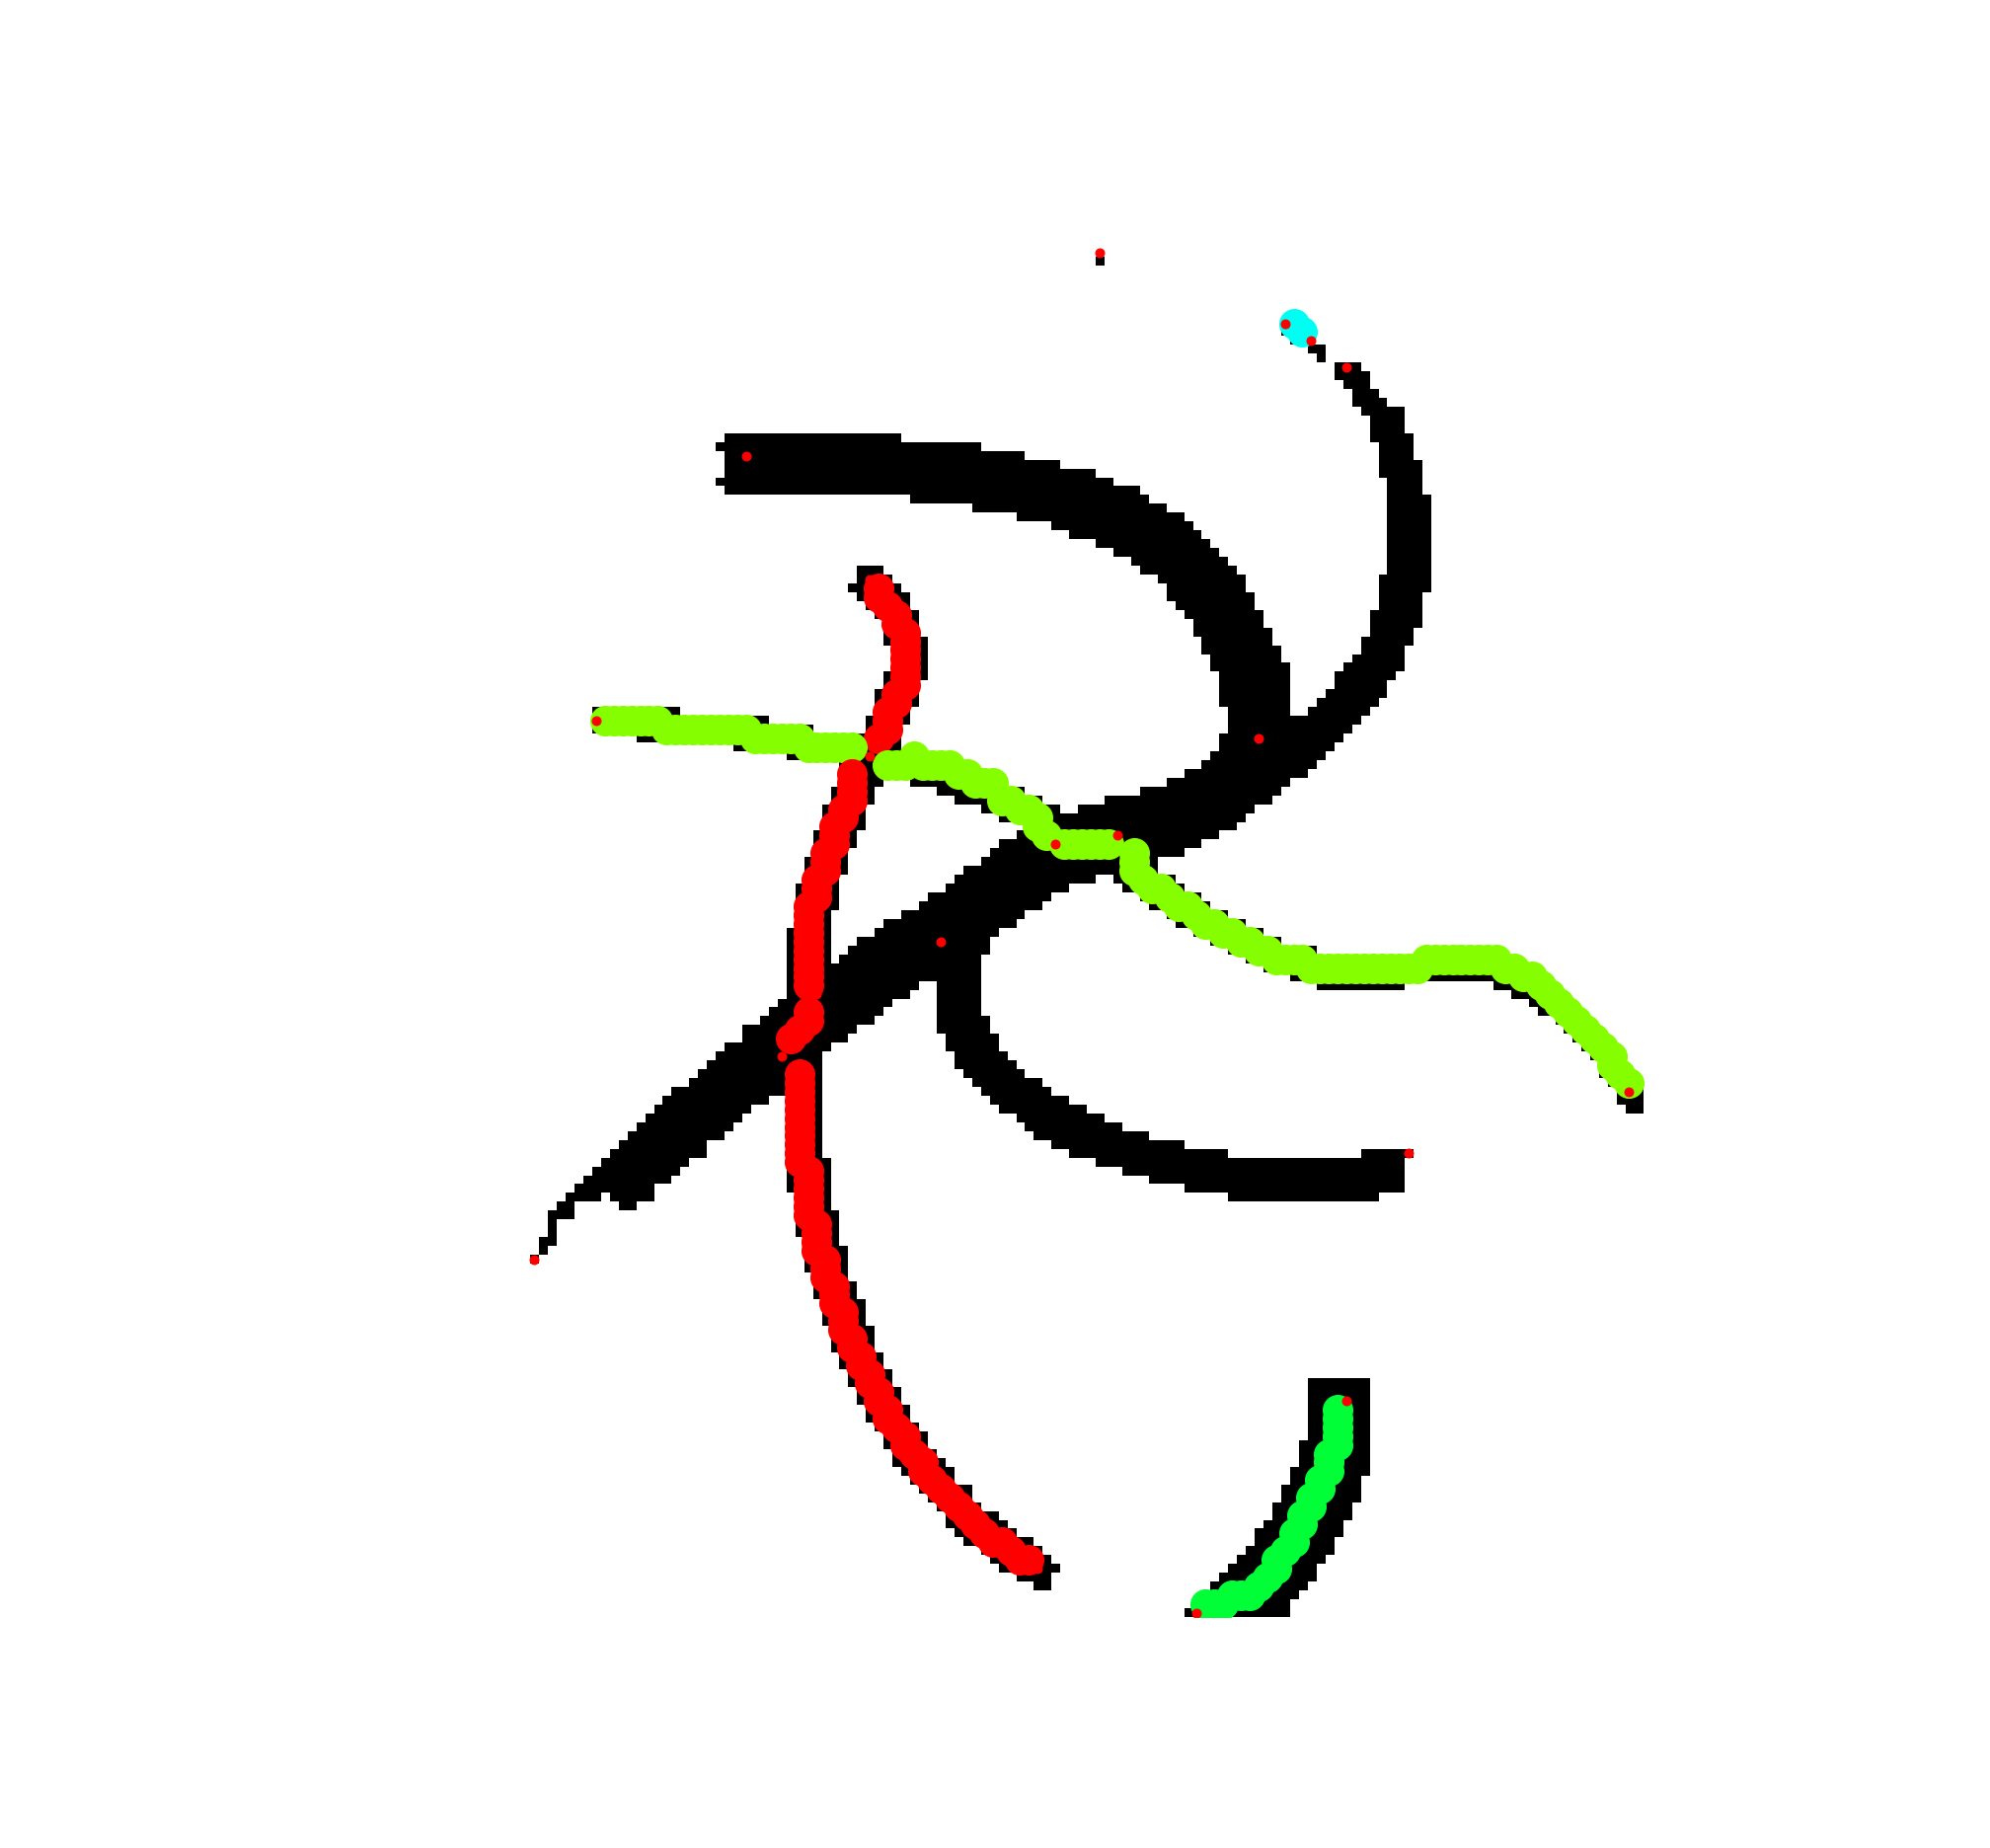
\includegraphics[scale=0.11]{resultImages/define-weighted-4-phil-s3389-v056-exactMatch-antLabeled.png}
        \caption{4 filamentos correctamente individualizados por el algoritmo propuesto con la configuraci\'on definida como Modo 4.}
        \label{fig:SynthDefine-Individualizacion-BestP2}
    \end{subfigure}
    
    \caption{Resultados de la individualizaci\'on de filamentos para la Figura \ref{fig:synth-Define-1b}, obtenidas mediante DeFiNe y el algoritmo propuesto, con diferentes par\'ametros. El algoritmo propuesto encuentra m\'as filamentos que los que se encuentran en las pruebas con DeFiNe. Sin embargo se aleja del comportamiento \'optimo indicado en \cite{breuer2015define}. Esta diferencia puede atribuirse a la excesiva curvatura de los filamentos sint\'eticos.}
    \label{fig:SynthDefine-Result}
\end{figure*}
\clearpage
\newpage
%%%%%%%%%% End Synth DeFiNe 1b %%%%%%%

\section{Im\'agenes Reales}

%recordar que define es base de BFS-Overlap-pairwise-total-
% recordarr que son 5 iteraciones y se estan promediando los resultados, conectar con la columna cobertura 
En esta secci\'on se muestran los resultados de la individualizaci\'on de filamentos para 2 tipos de c\'elulas, los microt\'ubulos existentes en la planta {\it Arabidopsis Marchantia}, y las dendritas en neuronas de rat\'on. Para cada tipo de c\'elulas existen 3 im\'agenes reales con las que se cuenta con la respectiva individualizaci\'on manual realizada por un experto. Se realizan pruebas utilizando las configuraciones predefinidas para estas c\'elulas en base a la informaci\'on recabada ante expertos.

\subsection{Microt\'ubulos de planta}
\label{subsec:mtTest}

%Valor m\'ax de VI para \ref{tab:SpinningMarchantiaResults1} es 3.4965.
%N\'umero de filamentos en el {\it Ground Truth} de la figura SpinningMarchanria es 12.
%Define y Phil presentan una propuesta de filamento para el ....

La primera evaluaci\'on corresponde a la muestra MT-A, indicada en la figura \ref{fig:SpinningMarchantia}, la que corresponde a una individualizaci\'on manual realizada por un experto a partir de una red de microt\'ubulos en la planta {\it Arabidopsis Marchantia}. La evaluaci\'on llevada a cabo mediante el algoritmo propuesto con los par\'ametros predefinidos para microt\'ubulos de planta para esta prueba se denomina Modo 5, y sus resultados, en conjunto con los resultados de DeFiNe se presentan en la Tabla \ref{tab:SpinningMarchantiaResults}.

De los 12 filamentos identificados por un experto, DeFiNe con un \'angulo de 30\textdegree~ individualiza 8 correctamente, mientras que con un \'angulo de 60\textdegree~ logra 3 individualizaciones correctas. Por su parte, el resultado del algoritmo propuesto con los par\'ametros predefinidos, indica que 4 de 5 pruebas individualizan al menos 7 filamentos correctamente, teniendo un caso donde se logran 8 aciertos. Lo anterior se refleja en la Figura \ref{fig:SpinningMarchantiaResults}. Se debe destacar que en 3 de las 4 pruebas que no logran encontrar el filamento adicional, existe una sobre-representaci\'on de aquel filamento ya que se le asigna una arista adicional, lo que lleva a no considerarlo como una respuesta correcta. 


Otros aspecto de estos resultados es que todas las evaluaciones logran una cobertura total de las aristas en sus propuestas de individualizaci\'on. Por su parte, las iteraciones durante el Modo 5 para el algoritmo propuesto, muestran estabilidad en el resultado para los par\'ametros predefinidos, logrando obtener la mayor\'ia de los filamentos que obtiene DeFiNe en sus 2 evaluaciones.

\begin{table}[h]
    \centering
    \begin{tabular}{|c|c|c|c|c|c|c|c|c|c|c|c|}
    \hline
          Algoritmo & P & P* & R & R* & F1 & F1* & C/P & C/P* & C/GT & C/GT* & T[s] \\ \hline
         DeFiNe 30\textdegree  & 0.65 & - & 0.45 & - & 0.53 & - & 8/16 & - & 8/12 & - & 4.10 \\
         DeFiNe 60\textdegree & 0.28 & - & 0.21 & - & 0.24 & - & 3/12 &- & 3/12 & - & 3.65\\
        Modo 5 & 0.44 & 0.45 & 0.34 & 0.35 & 0.38 & 0.4 & 7.2/12.4 & 8/13 & 7.2/12 & 8/12 & 0.35\\
         \hline
    \end{tabular}
    \caption{Resultados de individualizaci\'on de filamentos para la muestra MT-A en la Figura \ref{fig:SpinningMarchantia}. El valor m\'aximo de VI en este caso es de 3.3672, ya que el tama\~no del {\it data set} es de 29 aristas. El n\'umero de filamentos en el {\it ground truth} es 12. Las columnas P y R representan {\it Precision} y {\it Recall} respectivamente, la columna C/P refleja el n\'umero de filamentos correctos con respecto a los propuestos por cada m\'etodo, mientras que la columna C/GT indica la relaci\'on entre los filamentos correctamente individualizados por el m\'etodo y el criterio del experto. Finalmente la columna T indica el tiempo de ejecuci\'on. Las columnas sin asterisco representan el promedio de las iteraciones del algoritmo propuesto, mientras que las dem\'as indican el resultado de la mejor de las 5 iteraciones. Dado que DeFiNe es ejecutado una sola vez con cada \'angulo, su valor se muestra en las columnas promedio.}
    \label{tab:SpinningMarchantiaResults}
\end{table}

\begin{figure*}[h!]
    \centering
    \begin{subfigure}[t]{0.49\textwidth}
        \centering
        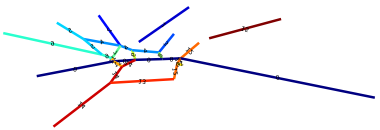
\includegraphics[scale=0.6]{resultImages/SpinningMarchantia-Define30.png}
        \caption{Individualizaci\'on obtenida mediante DeFiNe con un \'angulo de 30\textdegree .}
        \label{fig:SpinningMarchantiaResults-define30}
    \end{subfigure}%
    ~ 
    \begin{subfigure}[t]{0.49\textwidth}
        \centering
        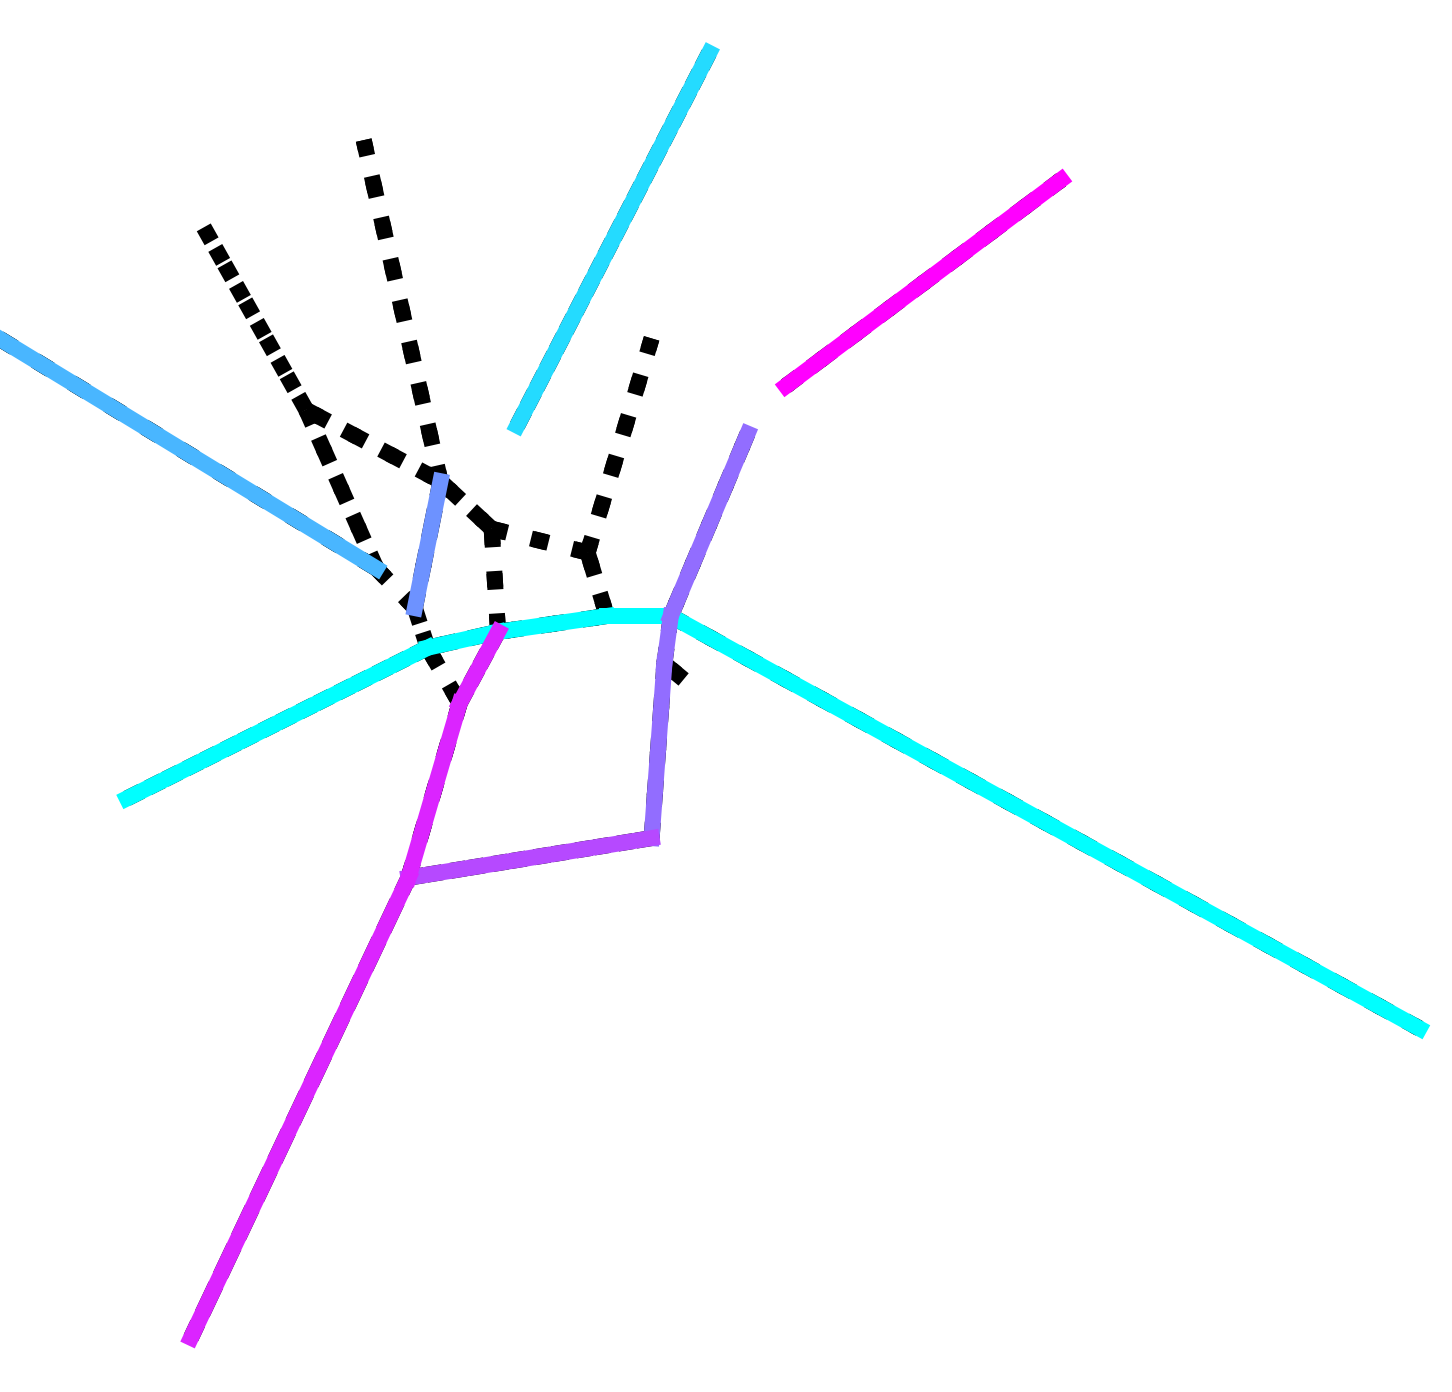
\includegraphics[height=1.3in]{resultImages/50-ROIs-Spinning-Marchantia-DeFiNeExactMatch-30.png}
        \caption{Representaci\'on de los filamentos correctamente individualizados en (a), identificados con colores.}
        \label{fig:SpinningMarchantiaResults-define30Exact}
    \end{subfigure}
    \vskip\baselineskip
    
    \begin{subfigure}[t]{0.49\textwidth}
        \centering
        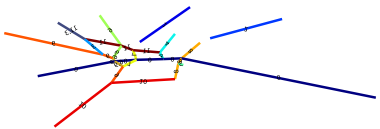
\includegraphics[scale=0.6]{resultImages/SpinningMarchantia-Define60.png}
        \caption{Individualizaci\'on obtenida mediante DeFiNe con un \'angulo de 60\textdegree .}
        \label{fig:SpinningMarchantiaResults-define60}
    \end{subfigure}
    ~ 
    \begin{subfigure}[t]{0.49\textwidth}
        \centering
        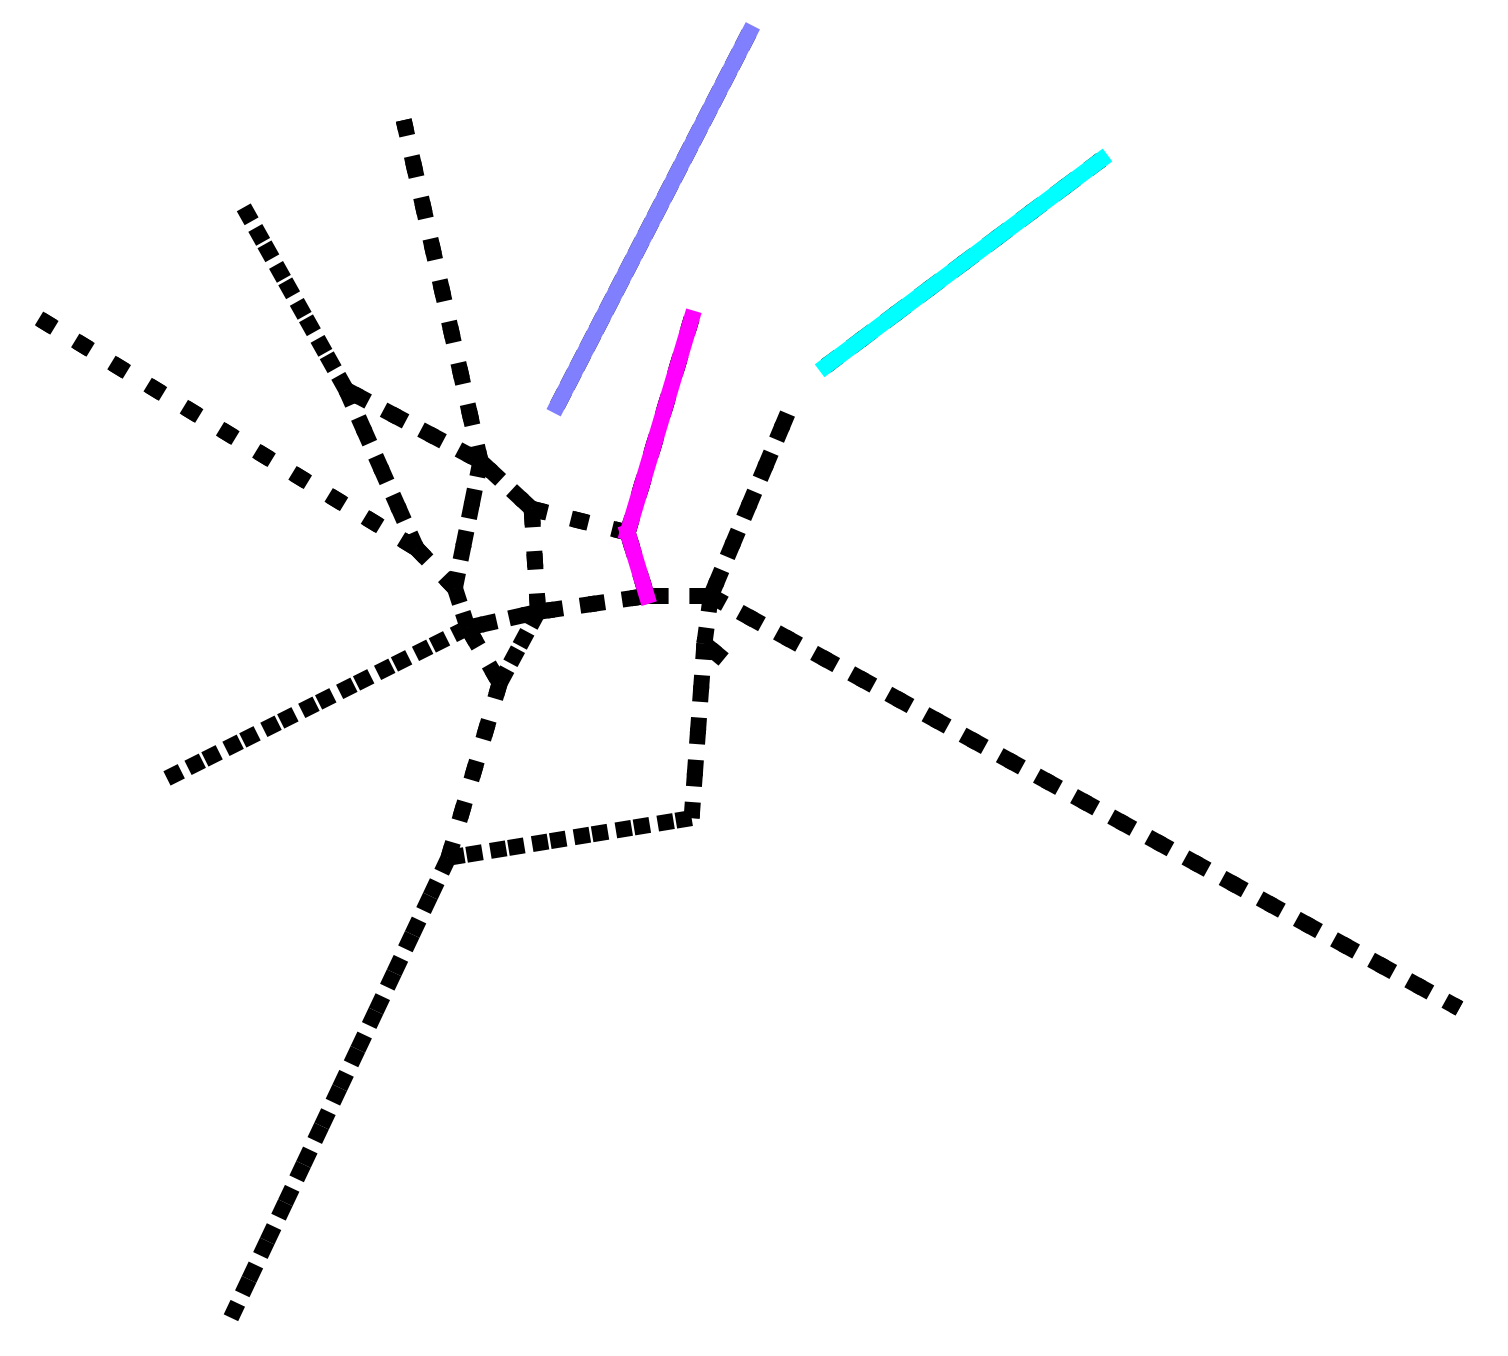
\includegraphics[height=1.3in]{resultImages/50-ROIs-Spinning-Marchantia-DeFiNeExactMatch-60.png}
        \caption{Representaci\'on de los filamentos correctamente individualizados en (c), identificados con colores.}
        \label{fig:SpinningMarchantiaResults-define60Exact}
    \end{subfigure}
    \vskip\baselineskip
    
    \begin{subfigure}[t]{0.49\textwidth}
        \centering
        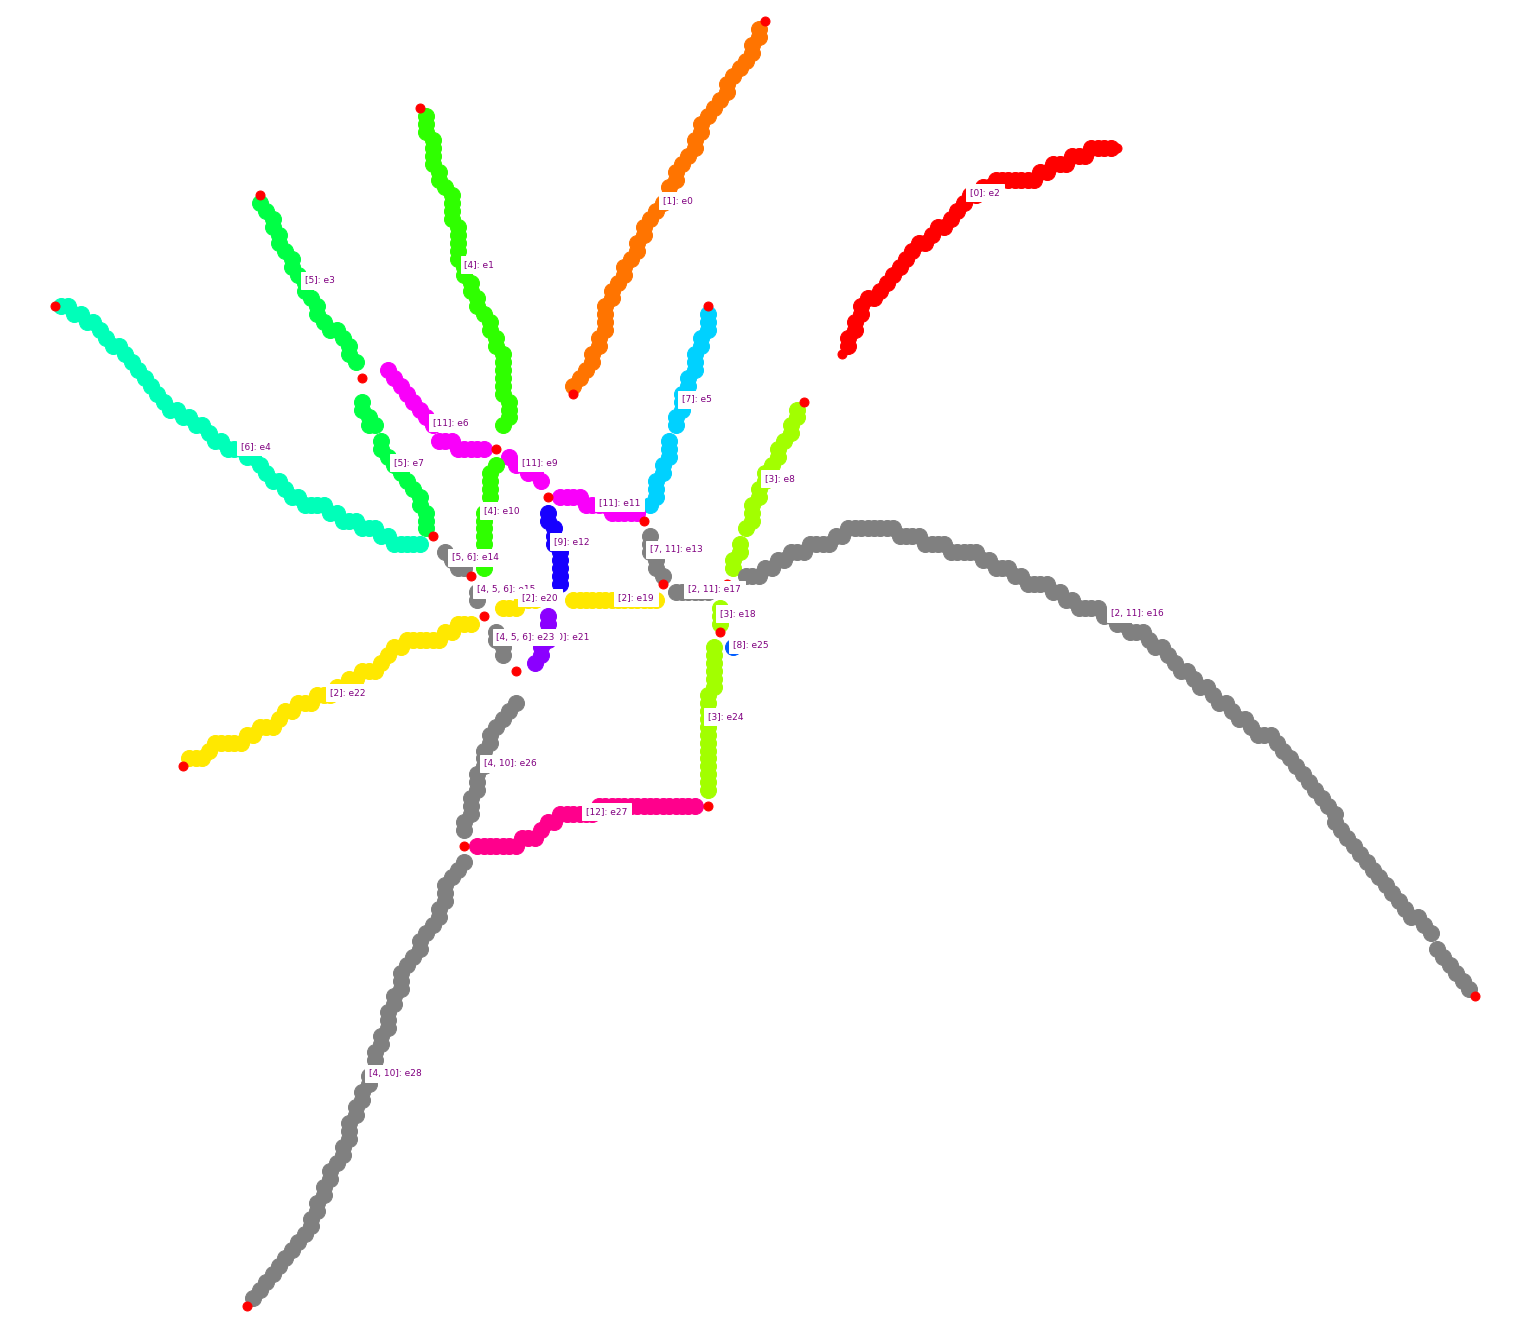
\includegraphics[height=1.4in]{resultImages/50-ROIs-Spinning-Marchantia-phil-s0-v05-nobg-antLabeled.png}
        \caption{Mejor resultado de la individualizaci\'on de filamentos usando el algoritmo propuesto con la configuraci\'on para microt\'ubulos de planta.}
        \label{SpinningMarchantiaResults-bestPhil}
    \end{subfigure}
    ~
    \begin{subfigure}[t]{0.49\textwidth}
        \centering
        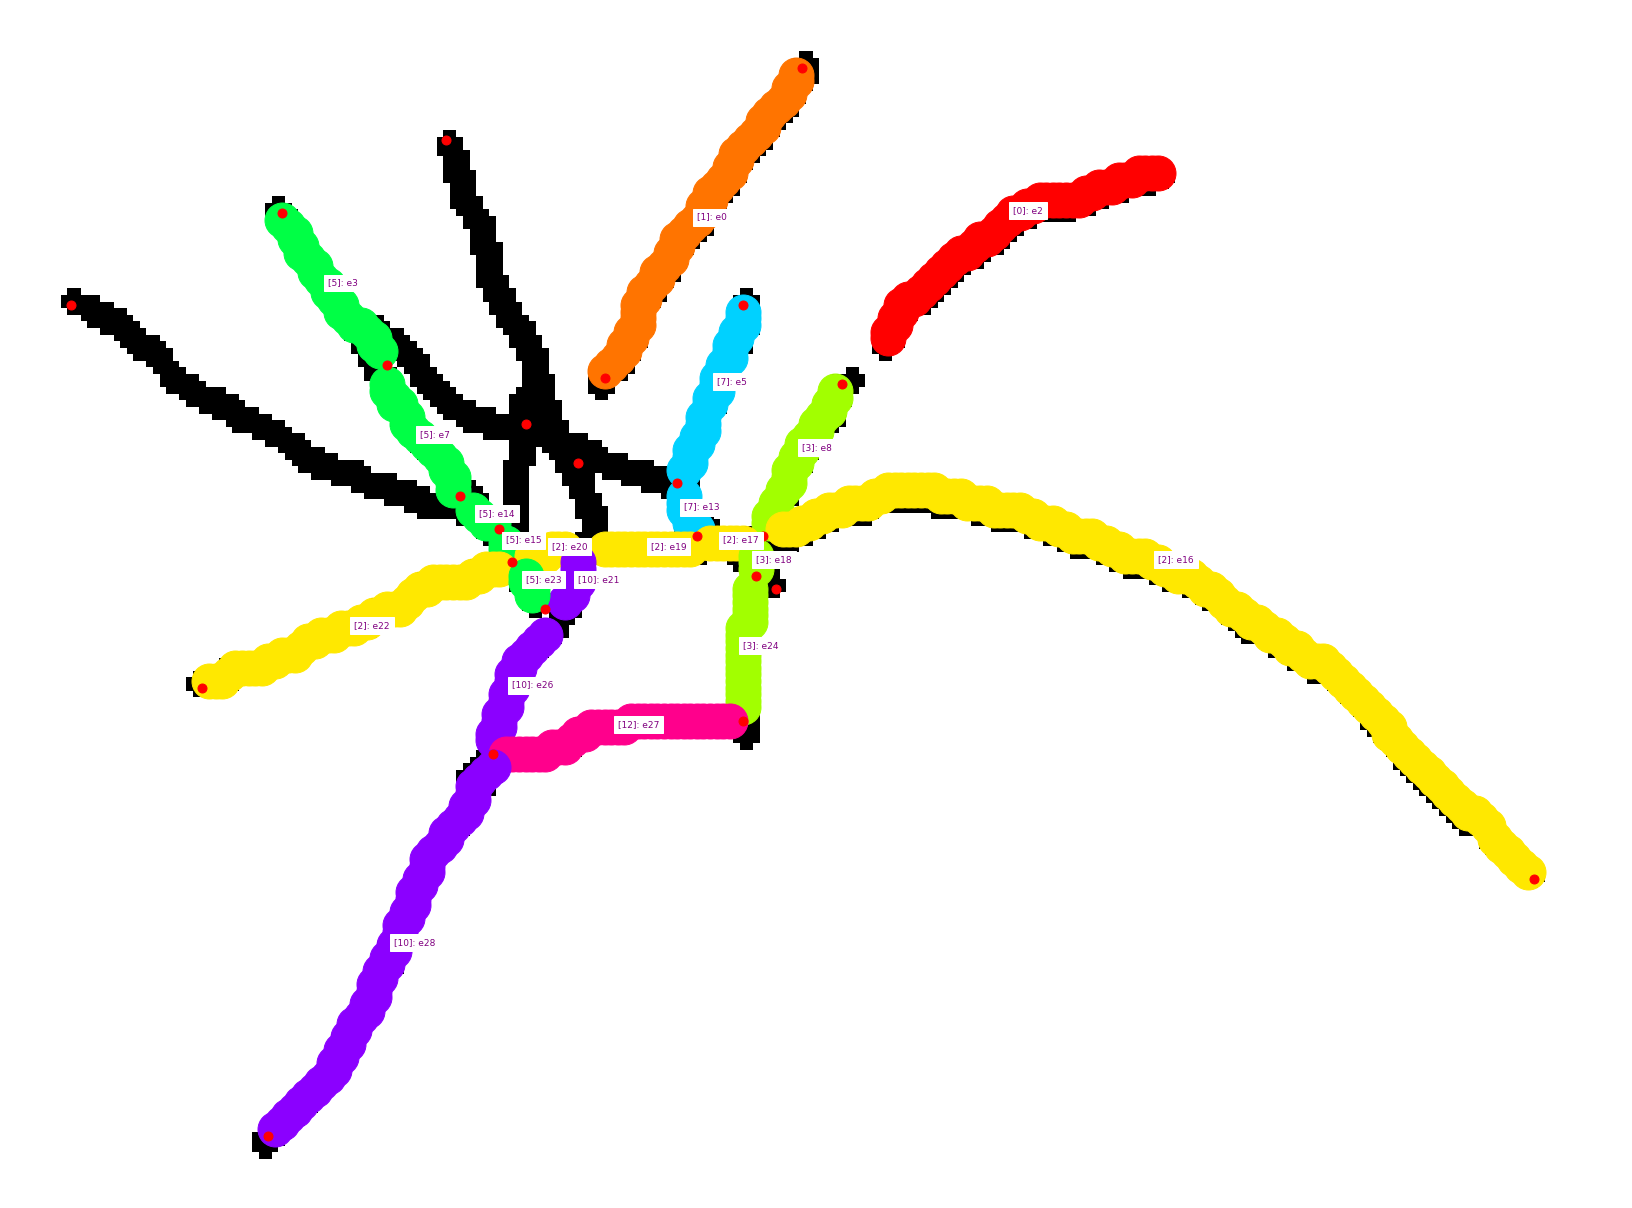
\includegraphics[height=1.4in]{resultImages/50-ROIs-Spinning-Marchantia-phil-s0-v05-exactMatch-antLabeled-thick.png}
        \caption{8 filamentos correctamente individualizados en base al resultado de (e).}
        \label{fig:SpinningMarchantiaResults-bestPhilExact}
    \end{subfigure}
    \vskip\baselineskip
    
    \begin{subfigure}[t]{0.49\textwidth}
        \centering
        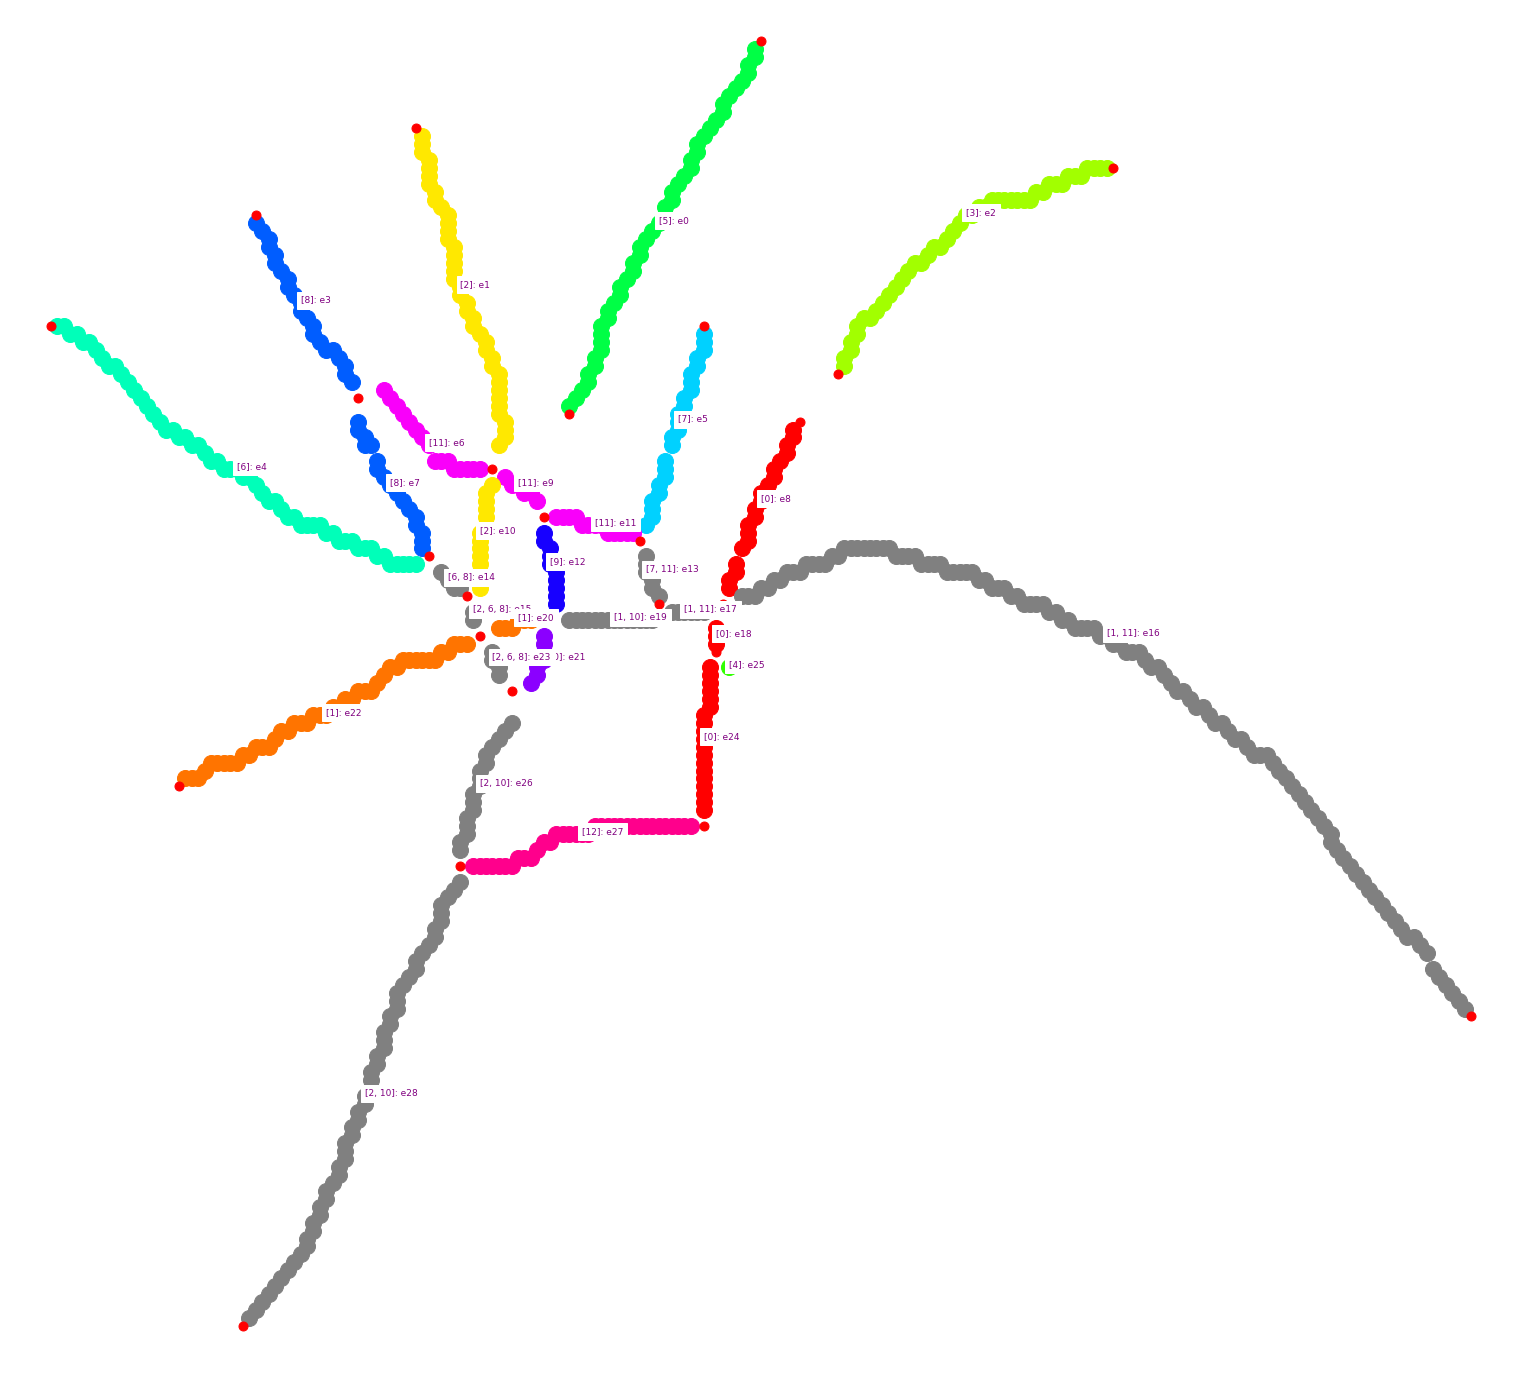
\includegraphics[height=1.4in]{resultImages/50-ROIs-Spinning-Marchantia-phil-s10-v05-nobg-antLabeled.png}
        \caption{Resultado promedio de la individualizaci\'on de filamentos usando el algoritmo propuesto con la configuraci\'on para microt\'ubulos de planta.}
        \label{SpinningMarchantiaResults-worstPhil}
    \end{subfigure}
    ~ 
    \begin{subfigure}[t]{0.49\textwidth}
        \centering
        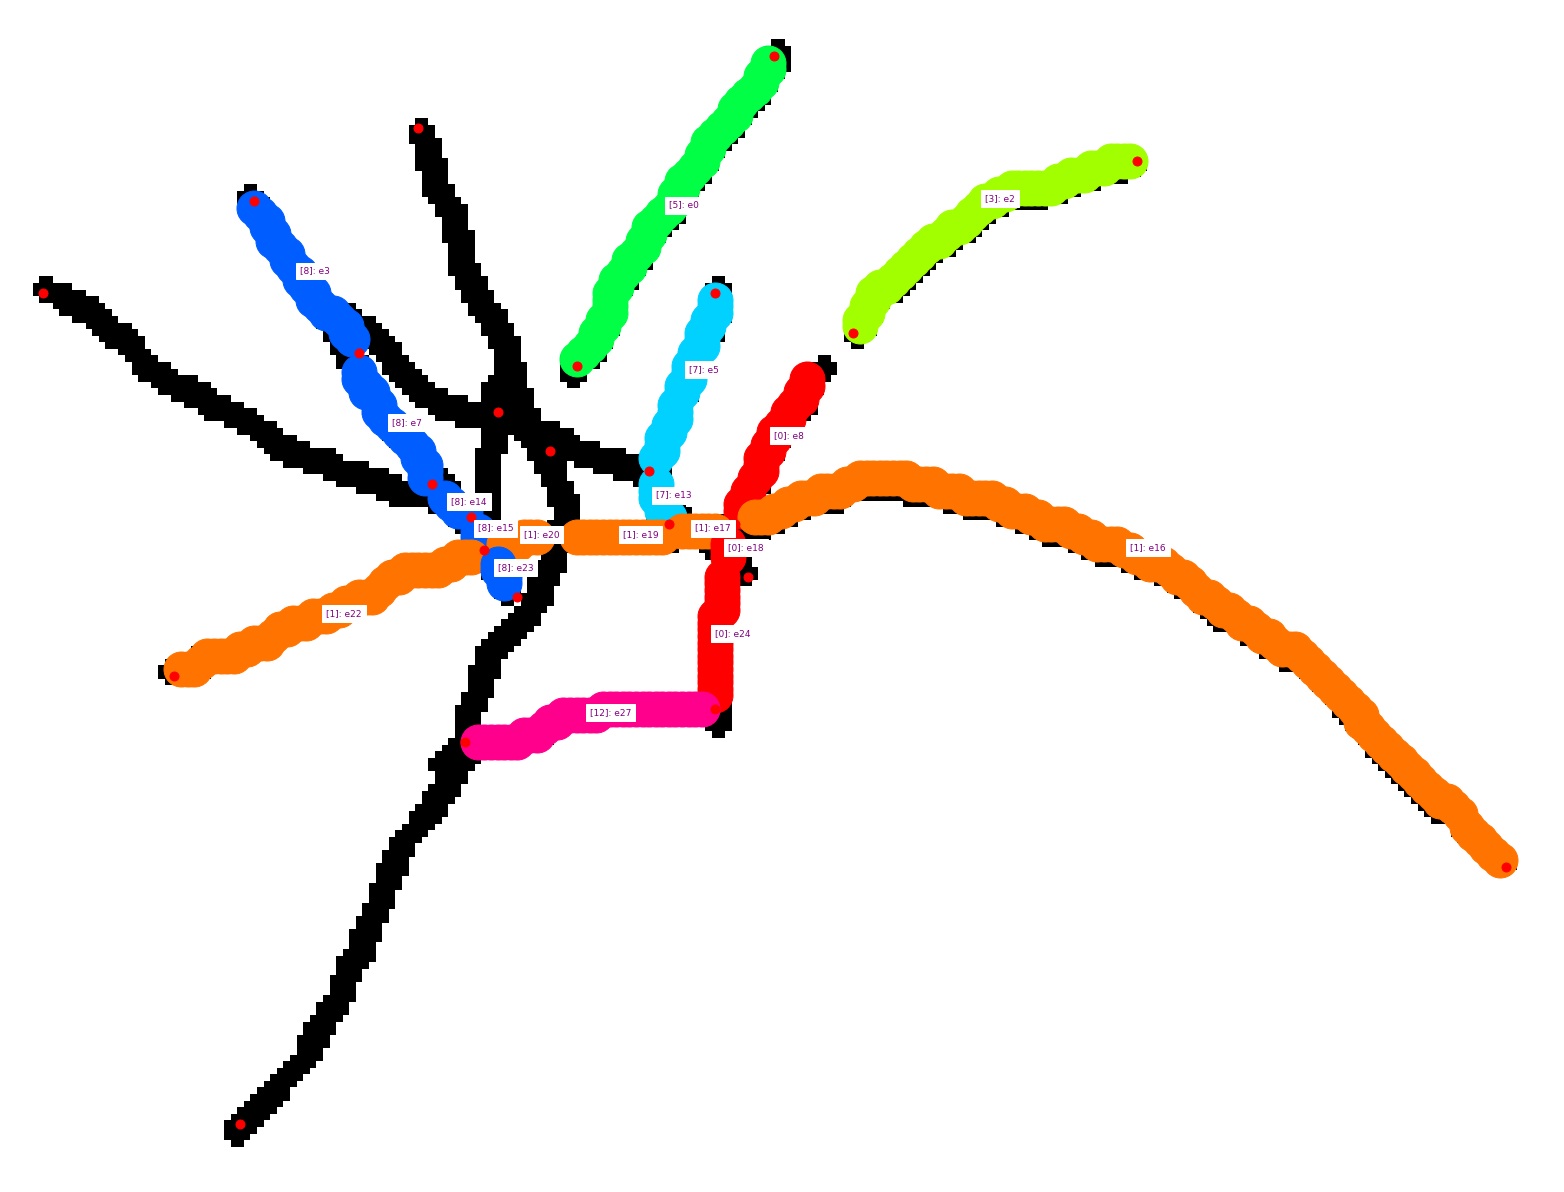
\includegraphics[height=1.4in]{resultImages/50-ROIs-Spinning-Marchantia-phil-s10-v05-exactMatch-antLabeled-thick.png}
        \caption{7 filamentos correctamente individualizados en base al resultado de (g).}
        \label{fig:SpinningMarchantiaResults-worstPhilExact}
    \end{subfigure}
    
    \caption{Filamentos propuestos y correctamente individualizados a partir la muestra MT-A en la Figura \ref{fig:SpinningMarchantia}, obtenidos mediante DeFiNe y el algoritmo propuesto con sus respectivos par\'ametros. Segmentos marcados en negro representan aristas no asignadas correctamente al filamento correspondiente en el {\it ground truth}, mientras que los filamentos correctamente identificados se encuentran identificados mediante colores.}
    \label{fig:SpinningMarchantiaResults}
\end{figure*}

\clearpage
\newpage


La segunda evaluaci\'on de microt\'ubulos de planta corresponde a la muestra MT-B, que se observa en la Figura \ref{fig:field3t0filtered1}, y cuya individualizaci\'on de filamentos usando el algoritmo propuesto se define como Modo 6. En base a los resultados del algoritmo propuesto, los que individualizan correctamente 8 filamentos en promedio, se observa la necesidad de un rango de tolerancia para determinar si una soluci\'on propuesta corresponde a un filamento. Esto se debe a que el grafo que representa la red de filamentos es una representaci\'on discreta, de la que pueden aparecer aristas que forman \'angulos por sobre los umbrales definidos, llevando a descartar estas soluciones sin su completa evaluaci\'on.

Un aspecto a destacar del algoritmo propuesto, radica que 4 de las 5 iteraciones del Modo 6 encuentran 9 filamentos, proponiendo 15 filamentos en promedio, lo que es menor a ambas evaluaciones realizadas con DeFiNe. A su vez, el algoritmo propuesto muestra un mejor desempe\~no en su tiempo de ejecuci\'on, demostrando poder soportar grafos de mayor n\'umero de nodos y aristas.

\begin{table}[h]
    \centering
    \begin{tabular}{|c|c|c|c|c|c|c|c|c|c|c|c|}
    \hline
          Algoritmo & P & P* & R & R* & F1 & F1* & C/P & C/P* & C/GT & C/GT* & T[s] \\ \hline
         DeFiNe 30\textdegree  & 0.51 & - & 0.17 & - & 0.26 & - & 5/23 & - & 5/12 & - & 5.03 \\
         DeFiNe 60\textdegree & 0.42 & - & 0.31 & - & 0.36 & - & 5/16 &- & 5/12 & - & 16.2\\
        Modo 6 & 0.5 & 0.52 & 0.32 & 0.40 & 0.39 & 0.45 & 8.8/15 & 9/14 & 8.8/12 & 9/12 & 0.96\\
        \hline
    \end{tabular}
    \caption{Resultados de la individualizaci\'on de filamentos para la muestra MT-B (Figura \ref{fig:field3t0filtered1}). El valor m\'aximo de VI en este caso es de 3.6888, ya que el n\'umero de aristas en el grafo utilizado es 40. 12 son los filamentos definidos por un experto. Las columnas P y R representan {\it Precision} y {\it Recall} respectivamente, la columna C/P refleja el n\'umero de filamentos correctos con respecto a los propuestos por cada m\'etodo, mientras que la columna C/GT indica la relaci\'on entre los filamentos correctamente individualizados por el m\'etodo y el criterio del experto. Finalmente la columna T indica el tiempo de ejecuci\'on. Las columnas sin asterisco representan el promedio de las iteraciones del algoritmo propuesto, mientras que las dem\'as indican el resultado de la mejor de las 5 iteraciones. Dado que DeFiNe es ejecutado una sola vez con cada \'angulo, su valor se muestra en las columnas promedio. El algoritmo propuesto presenta un comportamiento favorable, presentando un n\'umero de filamentos propuestos cercano a la cantidad de filamentos correctos.}
    \label{tab:field3t0filtered1}
\end{table}


\begin{figure*}[h!]
    \centering
    \begin{subfigure}[t]{0.49\textwidth}
        \centering
        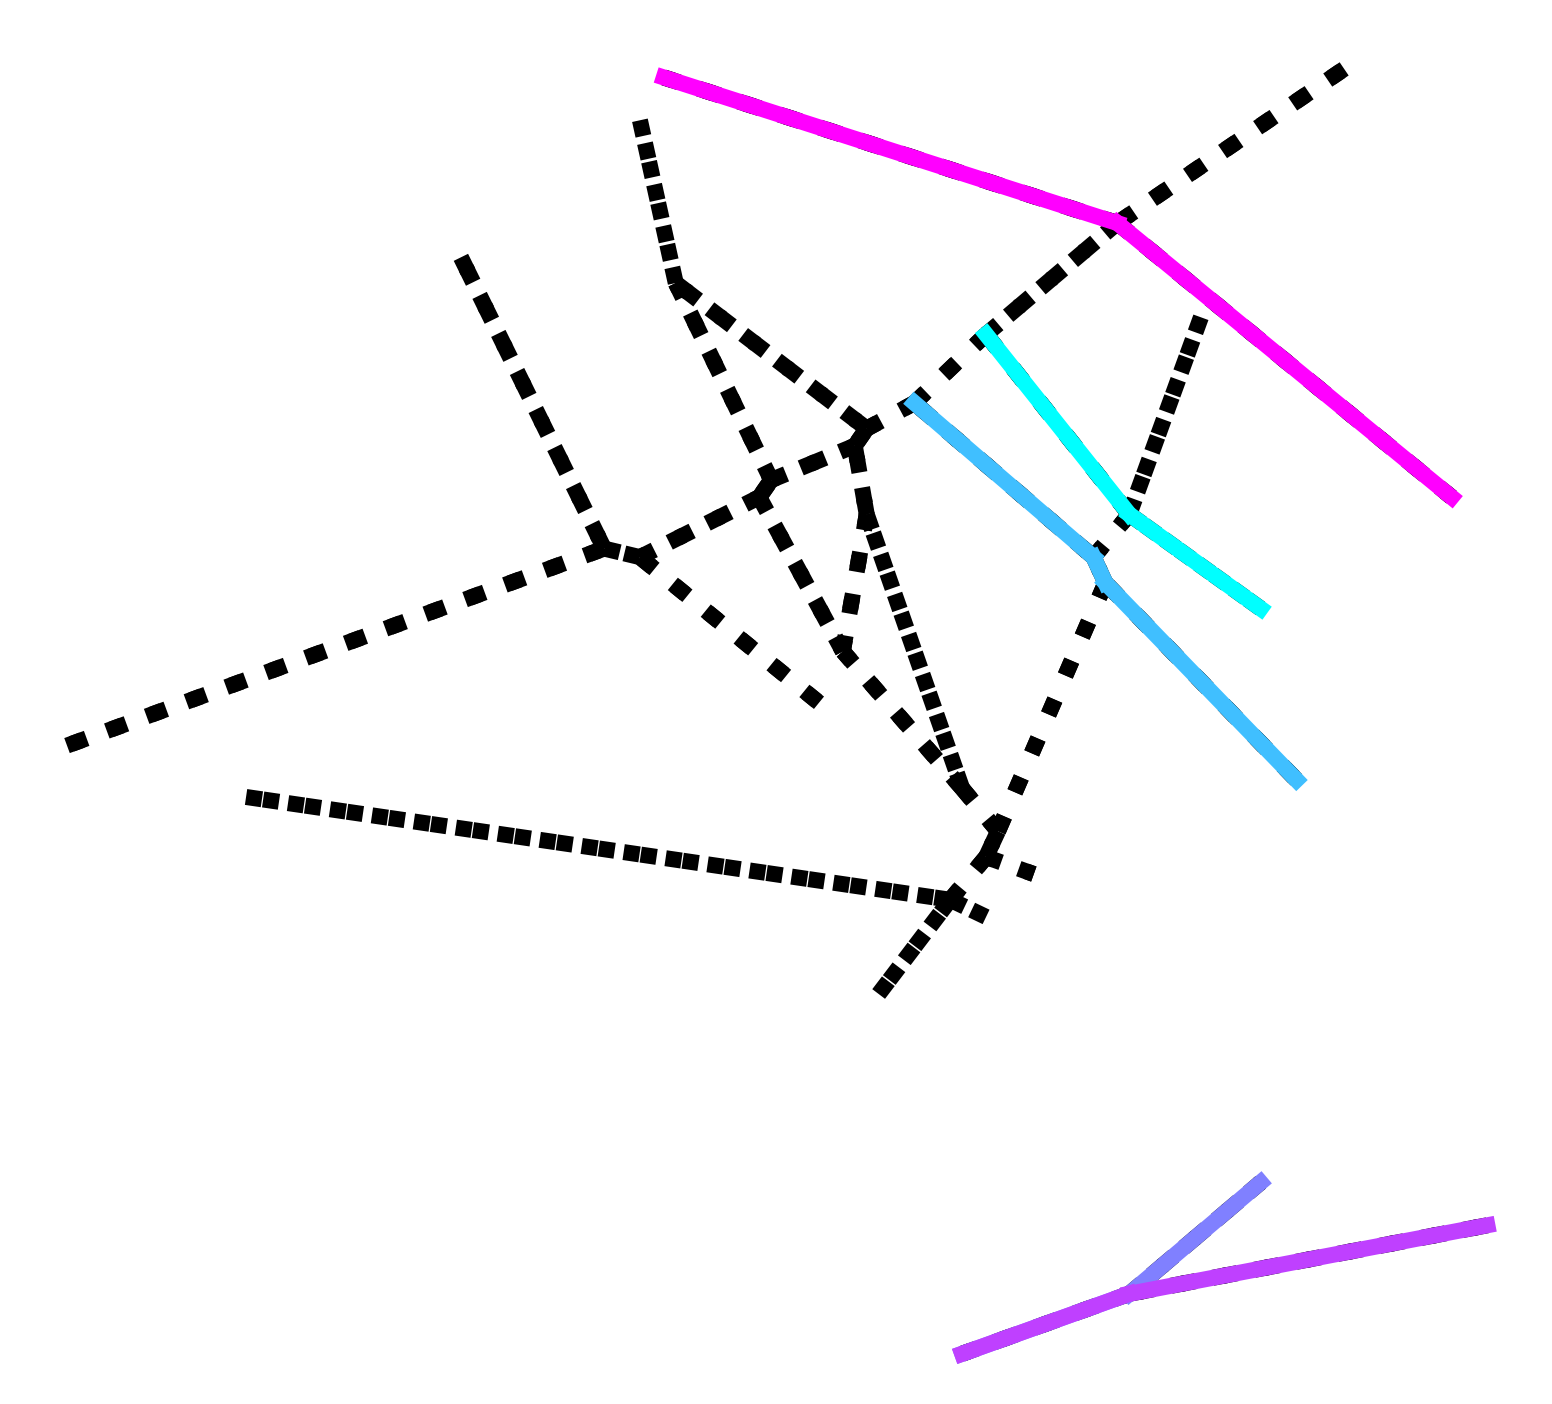
\includegraphics[height=1.5in]{resultImages/field3-t0-2cellBcrop-filtered-DeFiNeExactMatch-30.png}
        \caption{Representaci\'on de los 5 filamentos correctamente individualizados por DeFiNe con 30\textdegree, identificados con colores}
        \label{fig:field3t0filtered1Results-define30Exact}
    \end{subfigure}
    ~ 
    \begin{subfigure}[t]{0.49\textwidth}
        \centering
        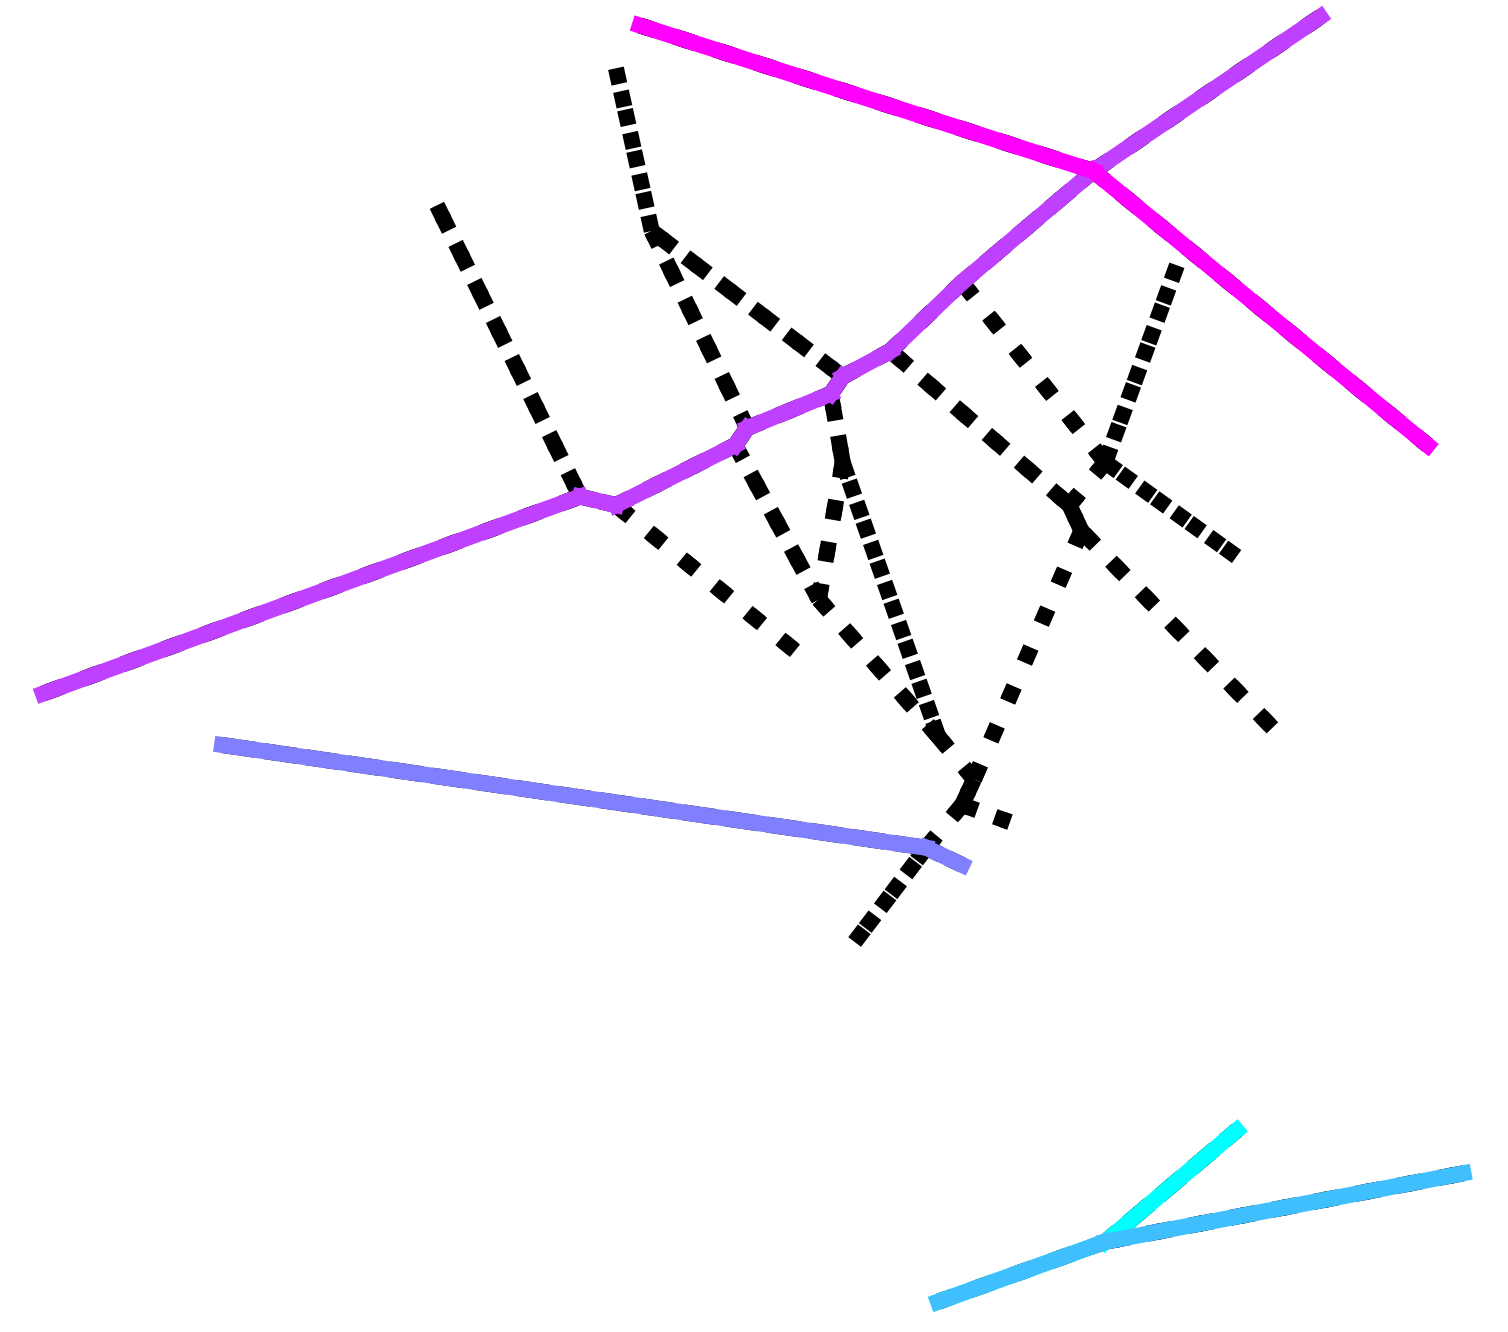
\includegraphics[height=1.5in]{resultImages/field3-t0-2cellBcrop-filtered-DeFiNeExactMatch-60.png}
        \caption{Representaci\'on de los 5 filamentos correctamente individualizados por DeFiNe con 60\textdegree, identificados con colores}
        \label{fig:field3t0filtered1Results-define60Exact}
    \end{subfigure}
    
    \vskip\baselineskip
    \begin{subfigure}[t]{0.49\textwidth}
        \centering
        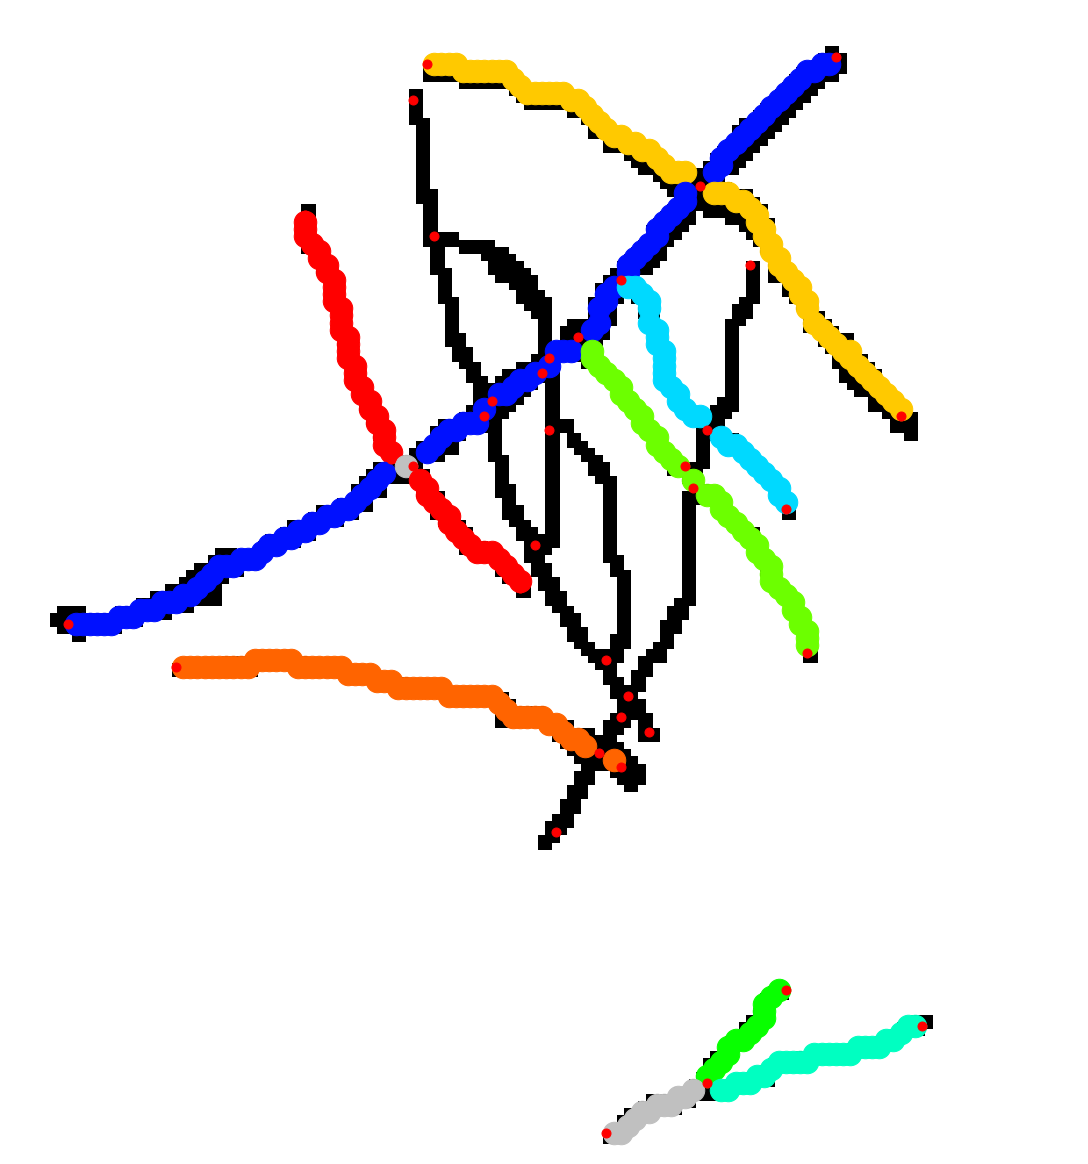
\includegraphics[height=1.5in]{resultImages/field3-t0-2cellBcrop-filtered-phil-s0-v056-exactMatch-antLabeled.png}
        \caption{Resultado promedio de Prueba 6, con 8 filamentos correctamente individualizados, identificados con colores.}
        \label{field3t0filtered1Results-bestPhil}
    \end{subfigure}
    ~ 
    \begin{subfigure}[t]{0.49\textwidth}
        \centering
        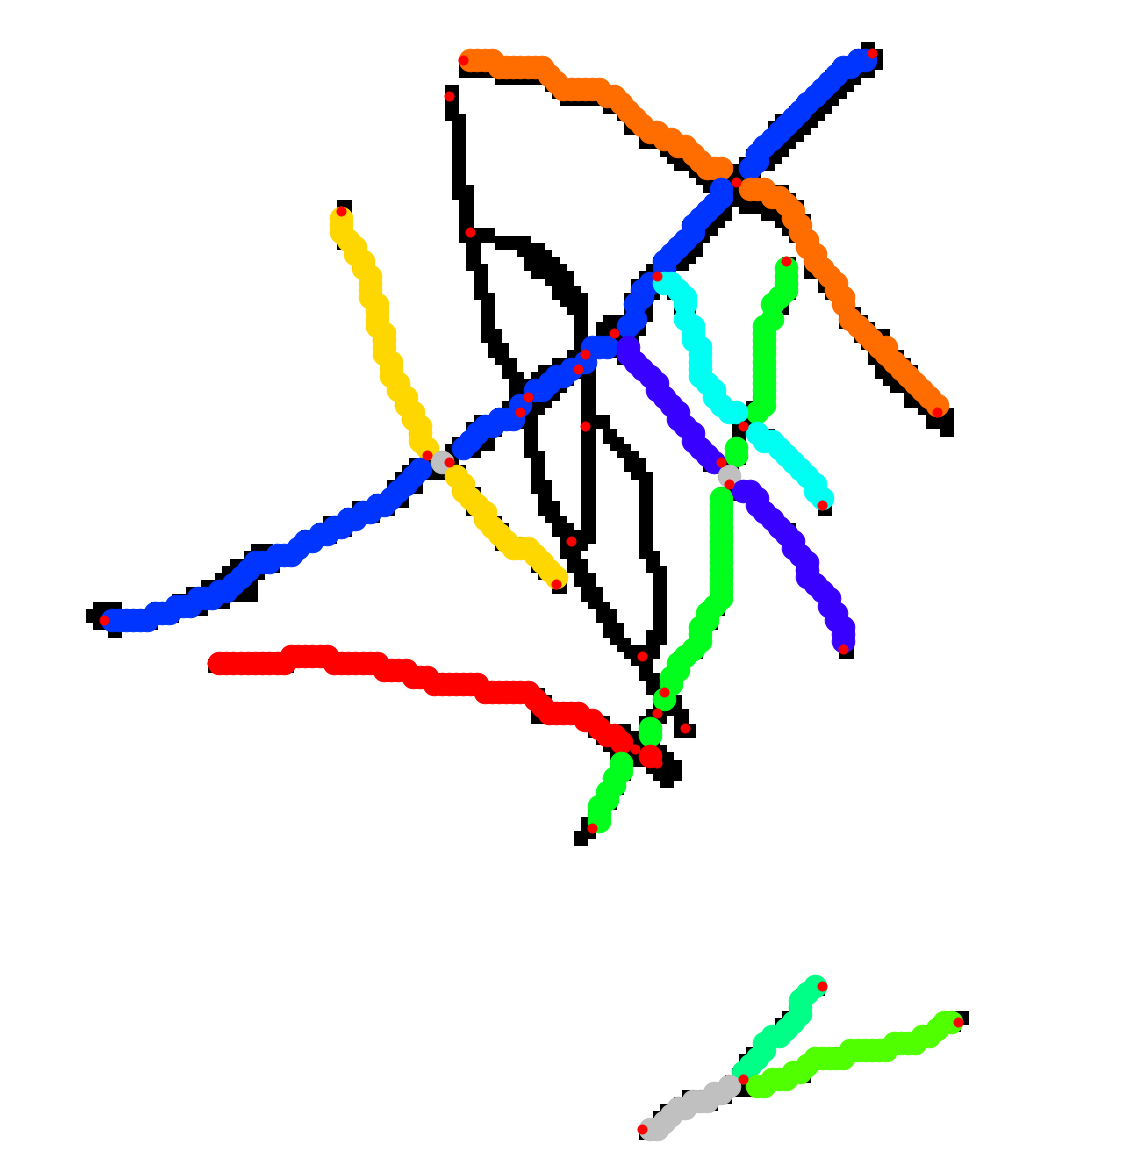
\includegraphics[height=1.5in]{resultImages/field3-t0-2cellBcrop-filtered-phil-s10-v056-exactMatch-antLabeled.png}
        \caption{9 Filamentos correctamente individualizados a partir del mejor resultado del algoritmo propuesto para la Prueba 6, identificados con colores.}
        \label{fig:field3t0filtered1Results-bestPhilExact}
    \end{subfigure}
    
    \caption{Filamentos correctamente individualizados en la figura \ref{fig:field3t0filtered1} correspondiente a la muestra MT-B, mediante el DeFiNe y el algoritmo propuesto. Segmentos marcados en negro representan aristas no asignadas correctamente. El mejor resultado del algoritmo propuesto permite encontrar filamentos no encontrados en a) o b).}
    \label{fig:field3t0filtered1Results}
\end{figure*}
\clearpage
\newpage

%Valor m\'ax de VI para \ref{tab:field3t0filtered2} es 1.9459.
%N\'umero de filamentos en el {\it Ground Truth} de la figura field3t0 es 5.

La individualizaci\'on de filamentos para la Figura \ref{fig:field3t0filtered2}, que representa la muestra MT-C, entrega los mismos resultados al ejecutar tanto DeFiNe con 60\textdegree~ como el algoritmo propuesto con los par\'ametros predefinidos para microt\'bulos de planta. Esta \'ultima evaluaci\'on se deonima Modo 7. Esto puede deberse a que la muestra MT-C es de mayor simplicidad que las muestras anteriores. Por su parte, la ejecuci\'on de DeFiNe con 30\textdegree~ individualiza correctamente 3 de 5 filamentos. Los resultados se indican en la Tabla \ref{tab:field3t0filtered2} y en l Figura \ref{fig:field3t0filtered2Results}.



El filamento faltante para el algoritmo propuesto corresponde a una sobre-asignaci\'on de aristas, similar a lo que ocurre en otras im\'agenes, llevando a no considerar aquella soluci\'on como un filamento valido. La posibilidad de sobre-asignar una arista a un filamento se condice con el comportamiento del algoritmo propuesto al favorecer la b\'usqueda de caminos/filamentos de mayor longitud que cumplan con el criterio de rectitud. Particularmente en este caso, un microt\'ubulo de planta puede corresponder a la fusi\'on de 2 microt\'ubulos en uno, denominado {\tt Zippering}, o al nacimiento de un microt\'ubulo a partir de uno existente, llamado {\tt Nucleaci\'on}. Ambas situaciones requieren de informaci\'on adicional para diferenciarlas, pudiendo usarse caracter\'isticas como el grosor de los segmentos de los filamentos involucrados en estas situaciones, as\'i como el \'angulo entre los segmentos de filamentos que se separan del segmento com\'un. La variaci\'on o continuidad del grosor y que el \'angulo mencionado se encuentre en un rango que var\'ia seg\'un el tipo de c\'elula son cr\'iticos para aclarar cual es el caso observado. 


%En relaci\'on al an\'alisis de las medidas y las m\'etricas en la tabla \ref{tab:field3t0filtered2}, se mantiene el empate entre DeFiNe-60\textdegree y Phil, con la \'unica diferencia en el tiempo de ejecuci\'on, favorable para Phil. 

\begin{table}[h]
    \centering
    \begin{tabular}{|c|c|c|c|c|c|c|c|c|c|c|c|}
    \hline
          Algoritmo & P & P* & R & R* & F1 & F1* & C/P & C/P* & C/GT & C/GT* & T[s] \\ \hline
         DeFiNe 30\textdegree  & 0.5 & - & 0.5 & - & 0.5 & - & 3/5 & - & 3/5 & - & 2.82 \\
         DeFiNe 60\textdegree & 0.55 & - & 0.5 & - & 0.57 & - & 4/5 &- & 4/5 & - & 2.65\\
        Modo 7 & 0.66 & 0.66 & 0.5 & 0.5 & 0.57 & 0.57 & 4/5 & 4/5 & 4/5 & 4/5 & 0.29\\
        \hline
    \end{tabular}
    \caption{Resultados de individualizaci\'on de filamentos para Figura \ref{fig:field3t0filtered2}, de la muestra MT-C. El valor m\'aximo de VI en este caso es de 1.9459, ya que existen 7 aristas en el grafo que representa la red de filamentos, y a su vez el n\'umero de filamentos correctos es 5. Las columnas P y R representan {\it Precision} y {\it Recall} respectivamente, la columna C/P refleja el n\'umero de filamentos correctos con respecto a los propuestos por cada m\'etodo, mientras que la columna C/GT indica la relaci\'on entre los filamentos correctamente individualizados por el m\'etodo y el criterio del experto. Finalmente la columna T indica el tiempo de ejecuci\'on. Las columnas sin asterisco representan el promedio de las iteraciones del algoritmo propuesto, mientras que las dem\'as indican el resultado de la mejor de las 5 iteraciones. Dado que DeFiNe es ejecutado una sola vez con cada \'angulo, su valor se muestra en las columnas promedio. Para esta muestra, todas las iteraciones del algoritmo propuesto obtienen el mismo resultado, los que tambi\'en sucede en la ejecuci\'on de DeFiNe con 60\textdegree, siendo la \'unica diferencia que el algoritmo propuesto realiza la individualizaci\'on en menor tiempo.}
    \label{tab:field3t0filtered2}
\end{table}

\begin{figure*}[h!]
    \centering
    \begin{subfigure}[t]{0.3\textwidth}
        \centering
        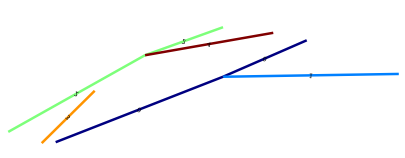
\includegraphics[scale=0.6]{resultImages/field3-t0-2cellBcrop-filtered-2-DeFiNe30.png}
        \caption{Individualizaci\'on mediante DeFiNe con 30\textdegree}
        \label{fig:field3t0filtered2Results-a}
    \end{subfigure}%
    ~ 
    \begin{subfigure}[t]{0.3\textwidth}
        \centering
        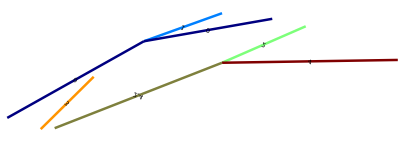
\includegraphics[scale=0.6]{resultImages/field3-t0-2cellBcrop-filtered-2-DeFiNe60.png}
        \caption{Individualizaci\'on mediante DeFiNe con 60\textdegree}
        \label{fig:field3t0filtered2Results-b}
    \end{subfigure}
    ~ 
    \begin{subfigure}[t]{0.3\textwidth}
        \centering
        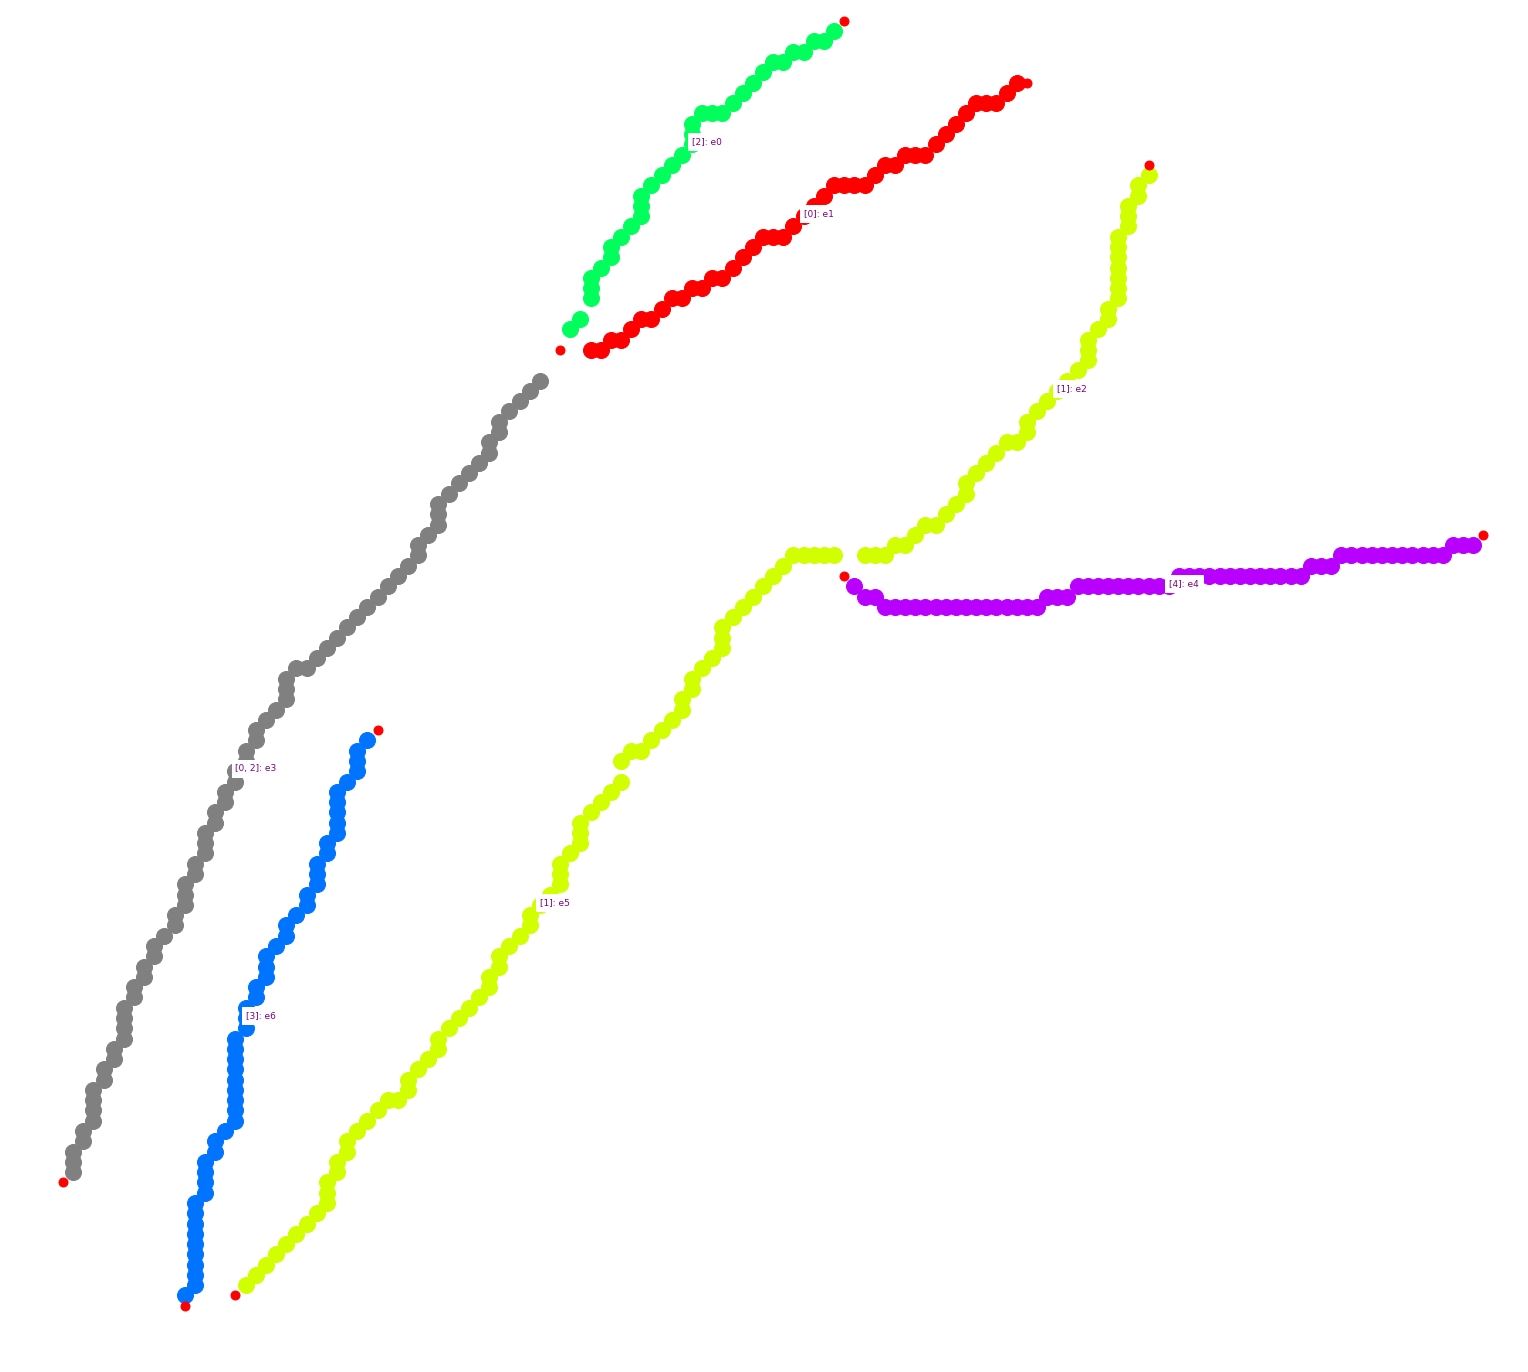
\includegraphics[height=1.5in]{resultImages/field3-t0-2cellBcrop-filtered-2-phil-s1271-v05-nobg-antLabeled.png}
        \caption{Individualizaci\'on de filamentos obtenida mediante el algoritmo propuesto, con los par\'ametros de microt\'ubulos de planta. El segmento plomo indica una arista seleccionada por m\'ultiples filamentos.}
        \label{fig:field3t0filtered2Results-c}
    \end{subfigure}
    \vskip\baselineskip
    
    \begin{subfigure}[t]{0.3\textwidth}
        \centering
        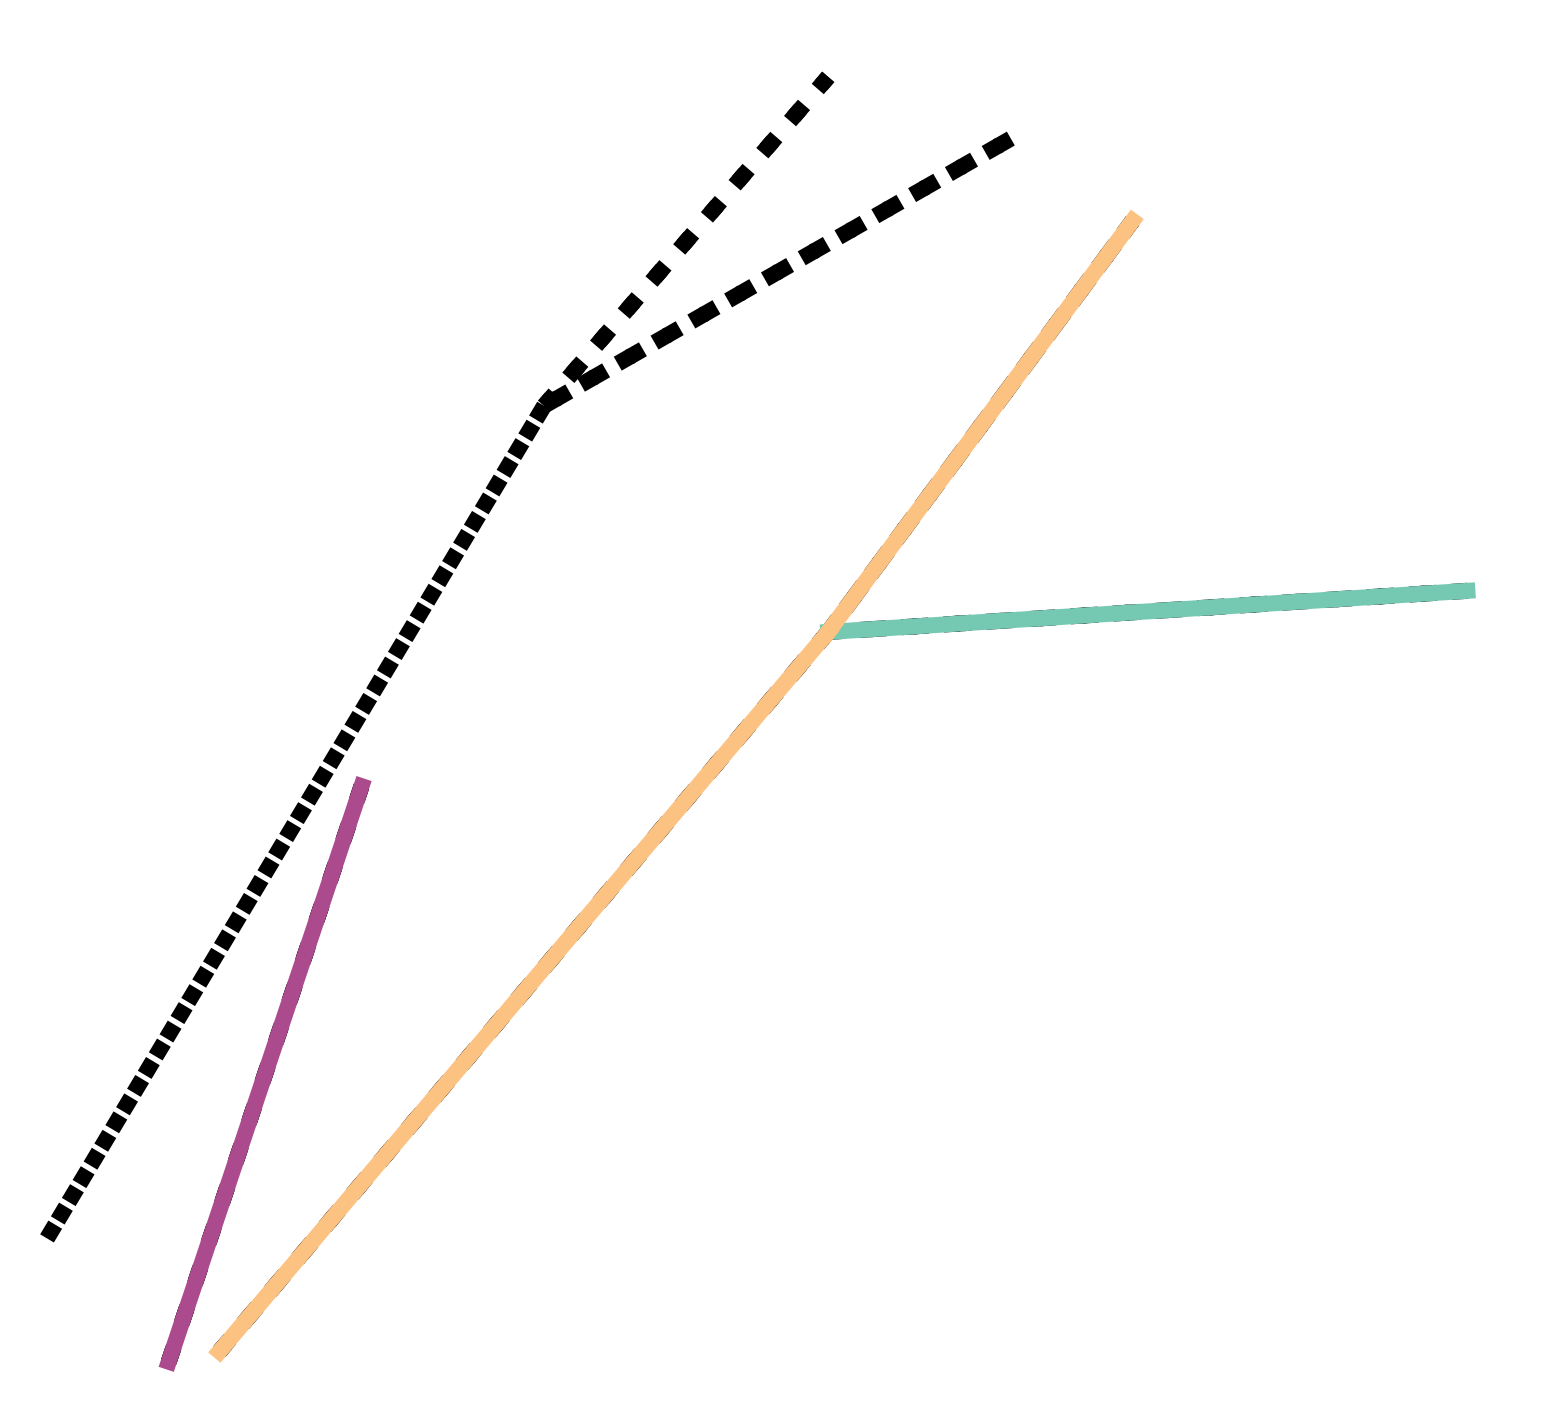
\includegraphics[height=1.5in]{resultImages/field3-t0-2cellBcrop-filtered-2-DeFiNeExactMatch-30.png}
        \caption{Representaci\'on de los filamentos correctamente individualizados en (a), identificados con colores}
        \label{fig:field3t0filtered2Results-d}
    \end{subfigure}%
    ~ 
    \begin{subfigure}[t]{0.3\textwidth}
        \centering
        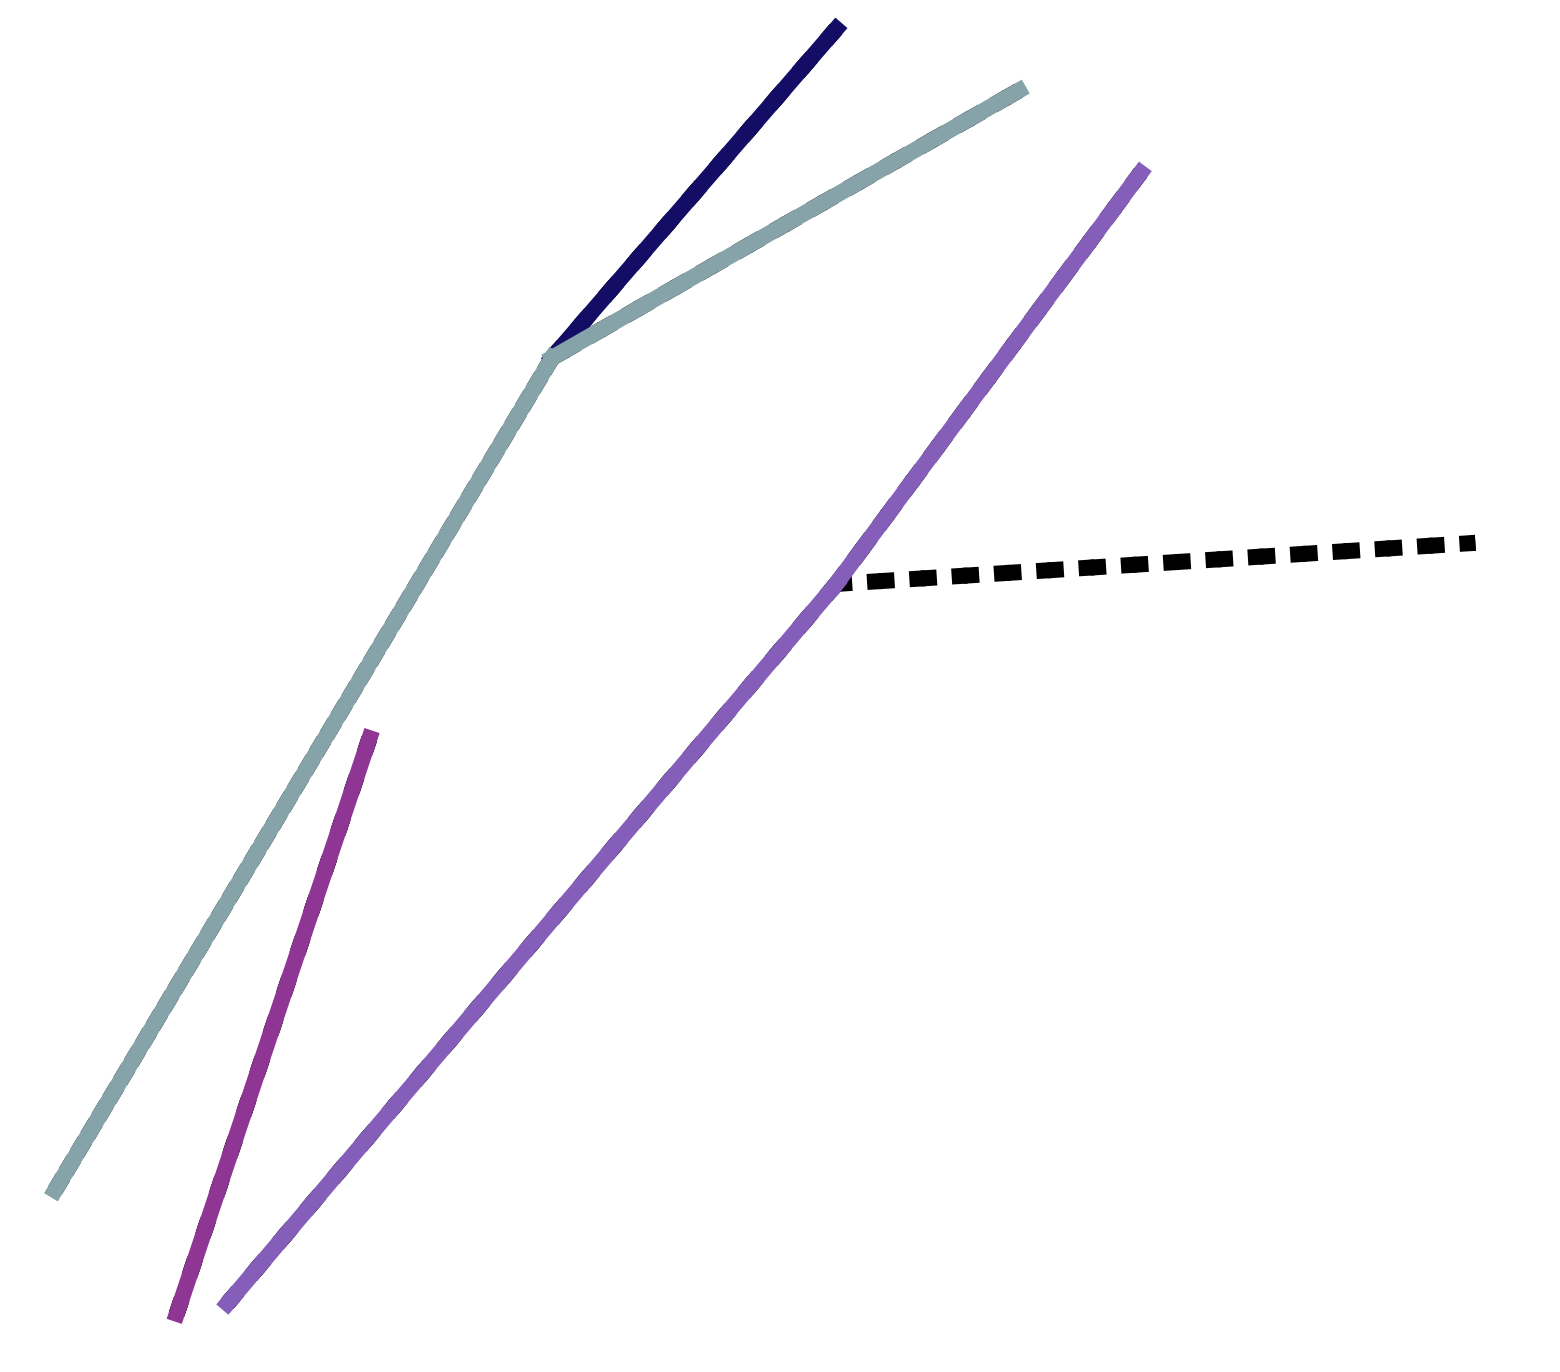
\includegraphics[height=1.5in]{resultImages/field3-t0-2cellBcrop-filtered-2-DeFiNeExactMatch-60.png}
        \caption{Representaci\'on de los filamentos correctamente individualizados en (b), identificados con colores}
        \label{fig:field3t0filtered2Results-e}
    \end{subfigure}
    ~ 
    \begin{subfigure}[t]{0.3\textwidth}
        \centering
        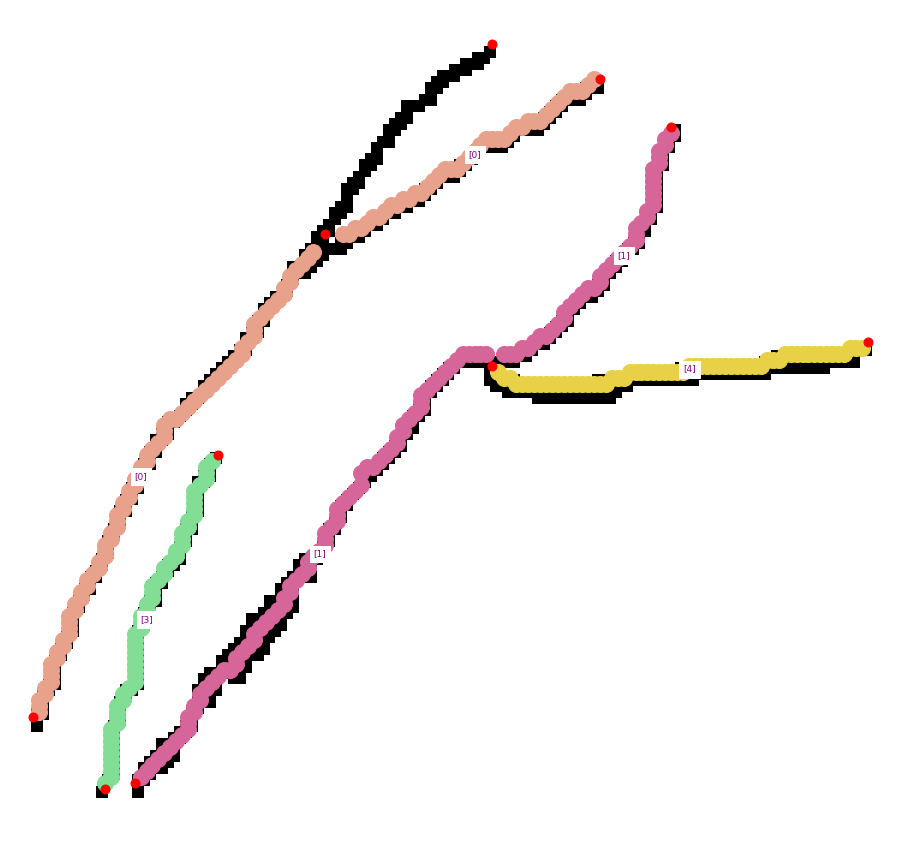
\includegraphics[height=1.5in]{resultImages/field3-t0-2cellBcrop-filtered-2-phil-s1271-v05-exactMatch-antLabeled.png}
        \caption{Filamentos correctamente individualizados en (c), identificados con colores}
        \label{fig:field3t0filtered2Results-f}
    \end{subfigure}
    
    \caption{Comparaci\'on entre filamentos propuestos y correctamente individualizados para la muestra MT-C en la Figura \ref{fig:field3t0filtered2}, con los distintos m\'etodos y par\'ametros. Segmentos marcados en negro representan aristas no asignadas correctamente al filamento correspondiente en el {\it ground truth.}. A pesar de la igualdad en resultados entre (e) y (f), el algoritmo propuesto lo obtiene en menor tiempo.}
    \label{fig:field3t0filtered2Results}
\end{figure*}

\clearpage
\newpage

\subsection{Neuronas}
\label{subsec:neuronTest}
En esta secci\'on se muestran los resultados de la evaluaci\'on del algoritmo propuesto para las 3 muestras de neuronas de rat\'on, obtenidas desde \cite{ampuero2019chronic}, y que se denominan N1, N2 y N3. Para estas 3 muestras se utiliza la configuraci\'on predeterminada de neurona de rat\'on. A diferencia de la secci\'on \ref{subsec:mtTest}, en estas evaluaciones las pruebas ejecutadas con DeFiNe presentan cantidades de filamentos propuestos 2 a 6 veces mayores que el n\'umero de filamentos individualizados por un experto. Este comportamiento puede atribuirse a la obligaci\'on que DeFiNe tiene de asignar todas las aristas al menos a un filamento. En comparaci\'on, el algoritmo propuesto al tener mayor flexibilidad, asigna en promedio un 57\% de las aristas a filamentos.

Adicionalmente, los tiempos de ejecuci\'on de las pruebas con DeFiNe son sustancialmente mayores, encontr\'andose en el rango de los minutos a las 4 horas, dependiendo de los par\'ametros utilizados. Lo anterior puede asociarse al n\'umero de aristas que las muestras de neurona tienen en su respectivo grafo, las que son 414 para N1 y 161 para N2. En el caso de la muestra N3, representada por un grafo de 67 aristas, esta no pudo ser calculada con DeFiNe ya que el programa arroja un error de falla cr\'itica, impidiendo su ejecuci\'on. La informaci\'on respecto al n\'umero de filamentos propuestos como de los tiempos de ejecuci\'on se encuentra en la Tabla \ref{tab:FilPropyTiemposNeuronasDefine}.

\begin{table}[h]
    \centering
    \begin{tabular}{|c|c|c|c|r|}
    \hline
         Muestra & Algoritmo & Fil. Propuestos & \% Asignaci\'on & Tiempo[s]\\
         \hline
         \multirow{3}{*}{N1}& DeFiNe 30\textdegree & 246 & 100 & 1514.6 \\
                            & DeFiNe 60\textdegree & 192 & 100 & 15573.7 \\
                            & Propuesto Promedio & 59 & 53.7 & 32.5 \\ \hline
        \multirow{3}{*}{N2}& DeFiNe 30\textdegree & 113 & 100 & 82.2 \\
                            & DeFiNe 60\textdegree & 85 & 100 & 456.4 \\
                            & Propuesto Promedio & 34.8 & 59.3 & 4.9 \\ \hline
                    N3 & Propuesto Promedio & 17.4 & 57.8 & 4.2 \\ \hline
    \end{tabular}
    \caption{N\'umero de filamentos propuestos y tiempos de ejecuci\'on para DeFiNe y el algoritmo propuesto promediado, para las muestras N1 y N2 en las Figuras \ref{fig:Porta6-4a1} y \ref{fig:Porta10-5b} respectivamente. Estas muestras contienen 24 y 29 filamentos cada una. La muestra N3 en la figura \ref{fig:Porta18-3a1} es representada por un grafo de 67 aristas y s\'olo considera los resultados promediados del algoritmo propuesto.}
    \label{tab:FilPropyTiemposNeuronasDefine}
\end{table}

As\'i, los motivos anteriores impiden realizar una evaluaci\'on con respecto al criterio experto, por lo que no se consideran los resultados de DeFiNe en esta secci\'on.

En cuanto a los resultados del algoritmo propuesto, indicados en la Tabla \ref{tab:neuronResults}, a pesar de ejecutar todas las evaluaciones en tiempos menores a 40 segundos, las individualizaciones correctas son bajas, mientras que el n\'umero de filamentos propuestos se acerca a la cantidad de filamentos individualizados manualmente por un experto, exceptuando el caso de la Muestra N1. Es posible asociar un comportamiento razonable del n\'umero de filamentos propuestos con la restricci\'on especial para neuronas considerada dentro de las penalizaci\'on de anti-feromonas, lo que permite mantener acotado el n\'umero de filamentos propuestos mediante el descarte de soluciones infactibles. Sin embargo, el bajo n\'umero de aciertos entre los filamentos propuestos refleja que la heur\'istica que influye en la probabilidad de elecci\'on de una arista durante la construcci\'on de caminos, indicada en la ecuaci\'on \ref{eq:heuristicaMiope}, no considera todas las caracter\'isticas necesarias para explorar exitosamente el grafo, en el caso de neuronas. 

Como se menciona en las evaluaciones previas, una de las mediciones principales es encontrar un calce exacto entre los filamentos propuestos y los que identifica el experto. Es por esto, que los filamentos que se sobre o sub asignan en 1 arista o m\'as no son considerados. Sin embargo, esta informaci\'on puede ser \'util para entender el m\'otivo por el cual un filamento propuesto queda tan cerca de ser un calce exacto con respecto a lo indicado por un experto. Esta informaci\'on adicional se encuentra en la columna F.S de la Tabla \ref{tab:neuronResults}, indicando que a\'un cuando los calces exactos son bajos, existen varios filamentos propuestos que se encuentran en un rango de 1 a 3 aristas faltantes o sobrantes, con respecto a un filamento correcto. Una comparaci\'on visual entre filamentos propuestos y correctos para las pruebas de esta secci\'on se encuentra en la Figura \ref{fig:NeuronPropVsCorrect}.

En las neuronas es observable la existencia de una dendrita de mayor longitud que el resto, denominada axón, a partir de la que nacen nuevas dendritas. A su vez, otras dendritas que nacen del centro de la neurona o soma, y se extienden de forma significativa tambi\'en sirven como lugar de nacimiento para nuevas dendritas. Este comportamiento implica la necesidad de considerar la selecci\'on de aristas que no s\'olo respeten el criterio de rectitud, sino que a la vez aporten con la mayor longitud al camino en construcci\'on.


\begin{table}[h]
    \centering
    \begin{tabular}{|c|c|c|c|c|c|c|c|c|c|c|c|c|}
    \hline
          Muestra & P & P* & R & R* & F1 & F1* & C/P & C/P* & C/GT & C/GT* & F.S. & F.S.* \\ \hline
        N1 & 0.62 & 0.6 & 0.15 & 0.13 & 0.24 & 0.22 & 1.6/59 & 3/66 & 1.6/24 & 3/24 & 1.4 & 1\\
        N2 & 0.2 & 0.21 & 0.09 & 0.1 & 0.13 & 0.14 & 4.6/34.8 & 6/34 & 4.6/29 & 6/29 & 8 & 7 \\
        N3 & 0.5 & 0.47 & 0.32 & 0.29 & 0.39 & 0.36 & 2/17.4 & 2/17 & 2/14 & 2/14 & 7.8 & 8\\
        \hline
    \end{tabular}
    
    \caption{Resultados de la individualizaci\'on de filamentos mediante el algoritmo propuesto para las muestra N1, N2 y N3, en las Figuras \ref{fig:Porta6-4a1}, \ref{fig:Porta10-5b} y \ref{fig:Porta18-3a1} respectivamente. Las columnas P y R representan {\it Precision} y {\it Recall} respectivamente, la columna C/P refleja el n\'umero de filamentos correctos con respecto a los propuestos por cada m\'etodo, mientras que la columna C/GT indica la relaci\'on entre los filamentos correctamente individualizados por el m\'etodo y el criterio del experto. Finalmente la La columna F.S. indica el n\'umero de filamentos sobre o sub asignados por a lo m\'as 3 arista. Las columnas sin asterisco representan el promedio de las iteraciones del algoritmo propuesto, mientras que las dem\'as indican el resultado de la mejor de las 5 iteraciones.}
    % Los valores m\'aximos de VI para cada muestra son 6.0258, 5.0814 y 4.2046, basados en el n\'umero de aristas de los grafos respectivos, que son 414 para N1, 161 para N2 y 67 para N3.
    \label{tab:neuronResults}
\end{table}




\begin{figure*}[h!]
    \centering
    \begin{subfigure}[t]{0.49\textwidth}
        \centering
        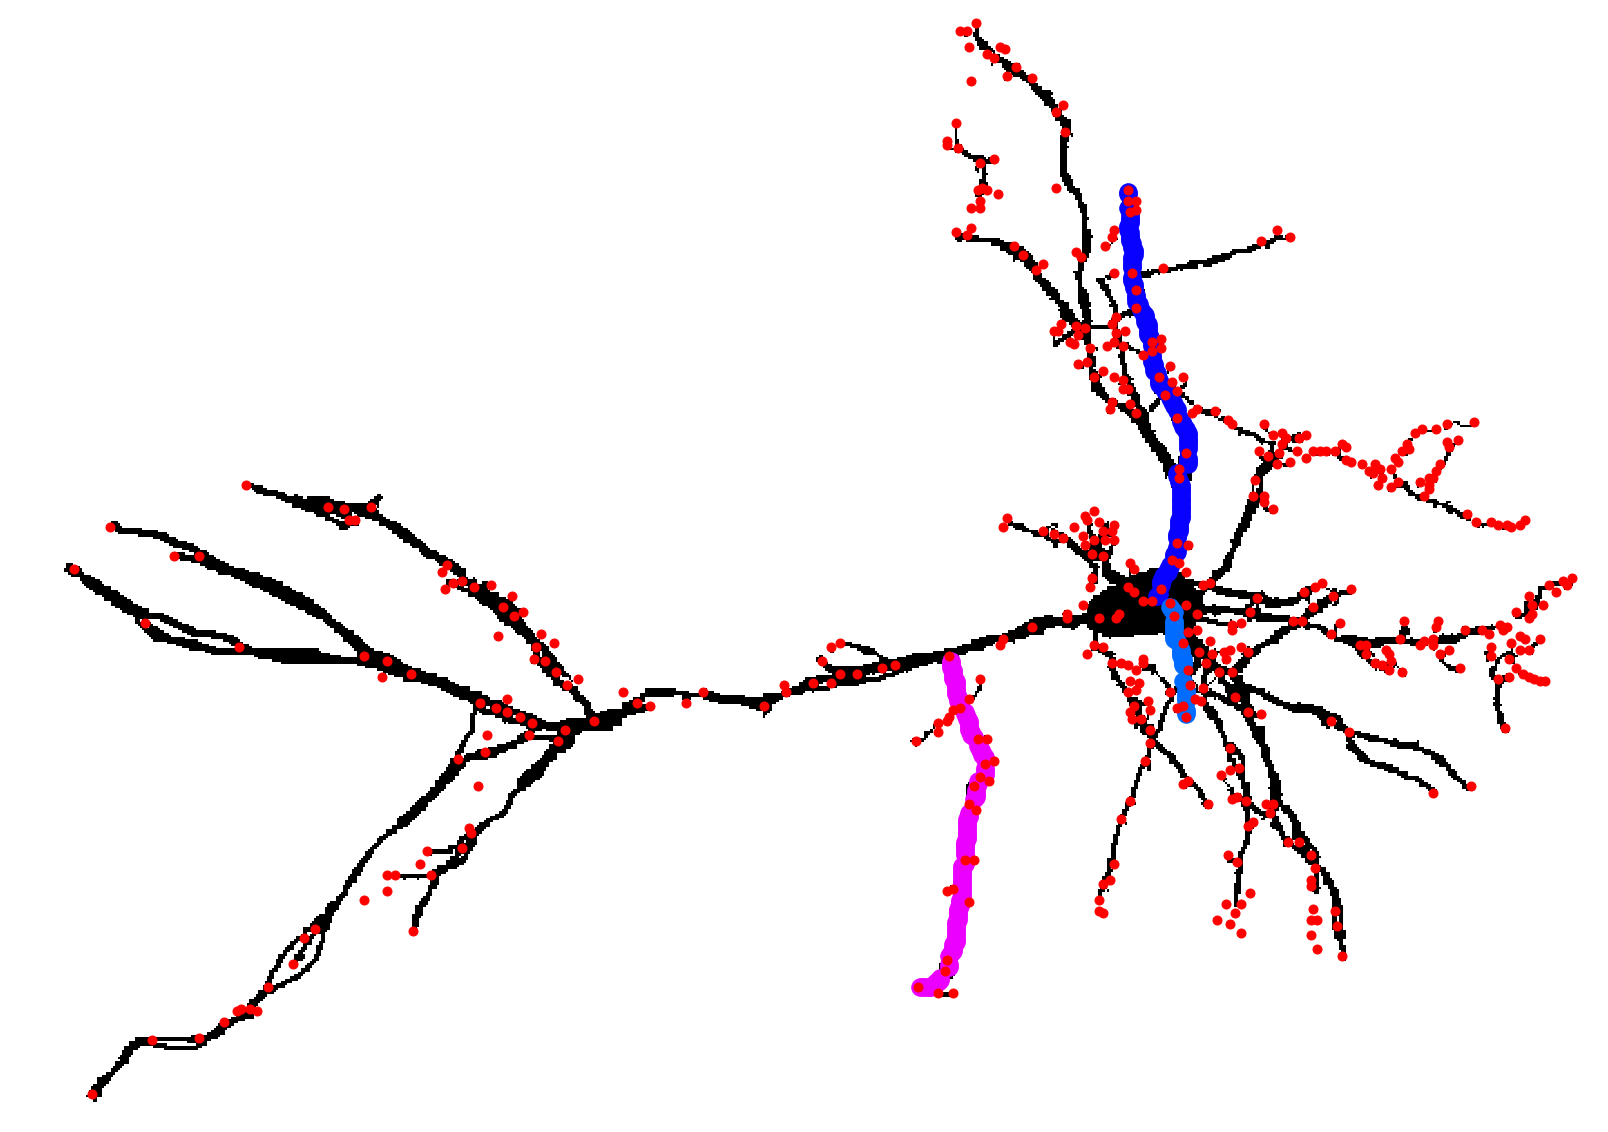
\includegraphics[height=1.5in]{resultImages/Porta6-4a1-phil-s10-v05-exactMatch-antLabeled.png}
        \caption{Filamentos correctamente individualizados por el algoritmo propuesto, para la muestra N1 en la Figura \ref{fig:Porta6-4a1}, identificados por colores.}
        \label{fig:Porta6Propuesta}
    \end{subfigure}
    ~ 
    \begin{subfigure}[t]{0.49\textwidth}
        \centering
        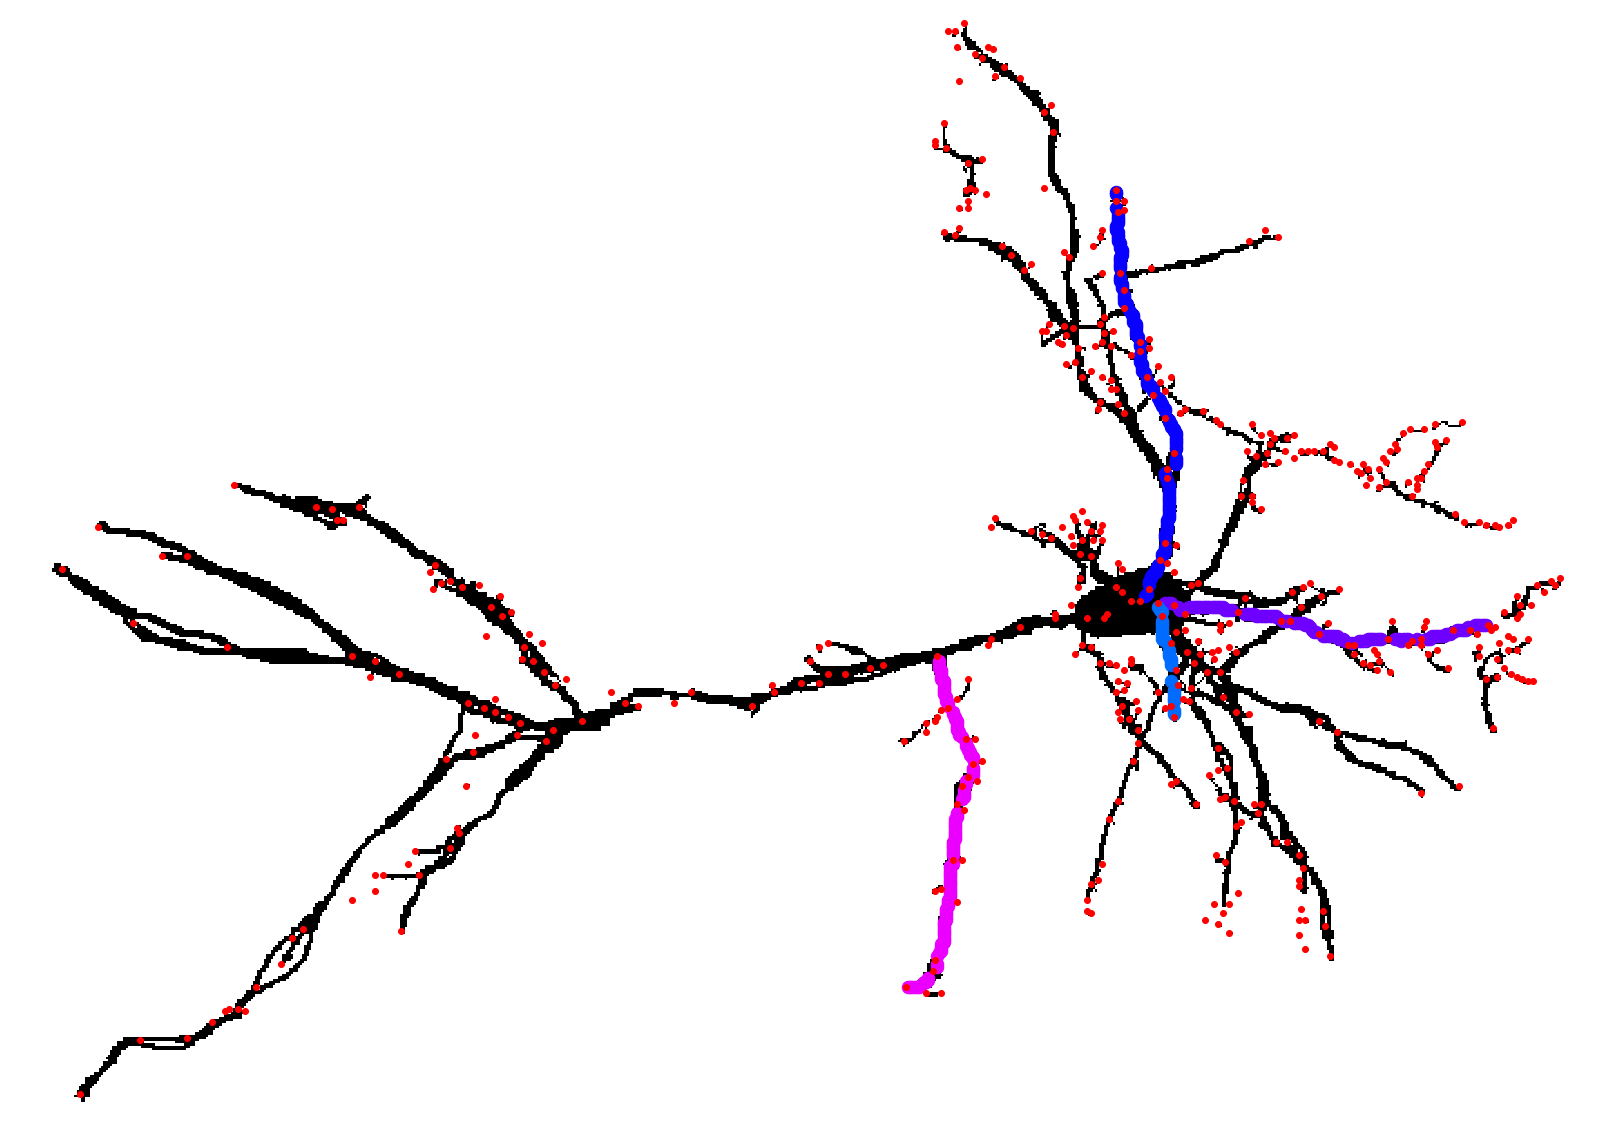
\includegraphics[height=1.5in]{resultImages/Porta6-4a1-phil-s10-v056-overmatches-3-antLabeled.png}
        \caption{Filamentos correctamente individualizados en (a) m\'as un filamentos sobre o sub asignados por 1 arista, a partir del resultado del algoritmo propuesto.}
        \label{fig:Porta6Best}
    \end{subfigure}
    
    \vskip\baselineskip
    \begin{subfigure}[t]{0.49\textwidth}
        \centering
        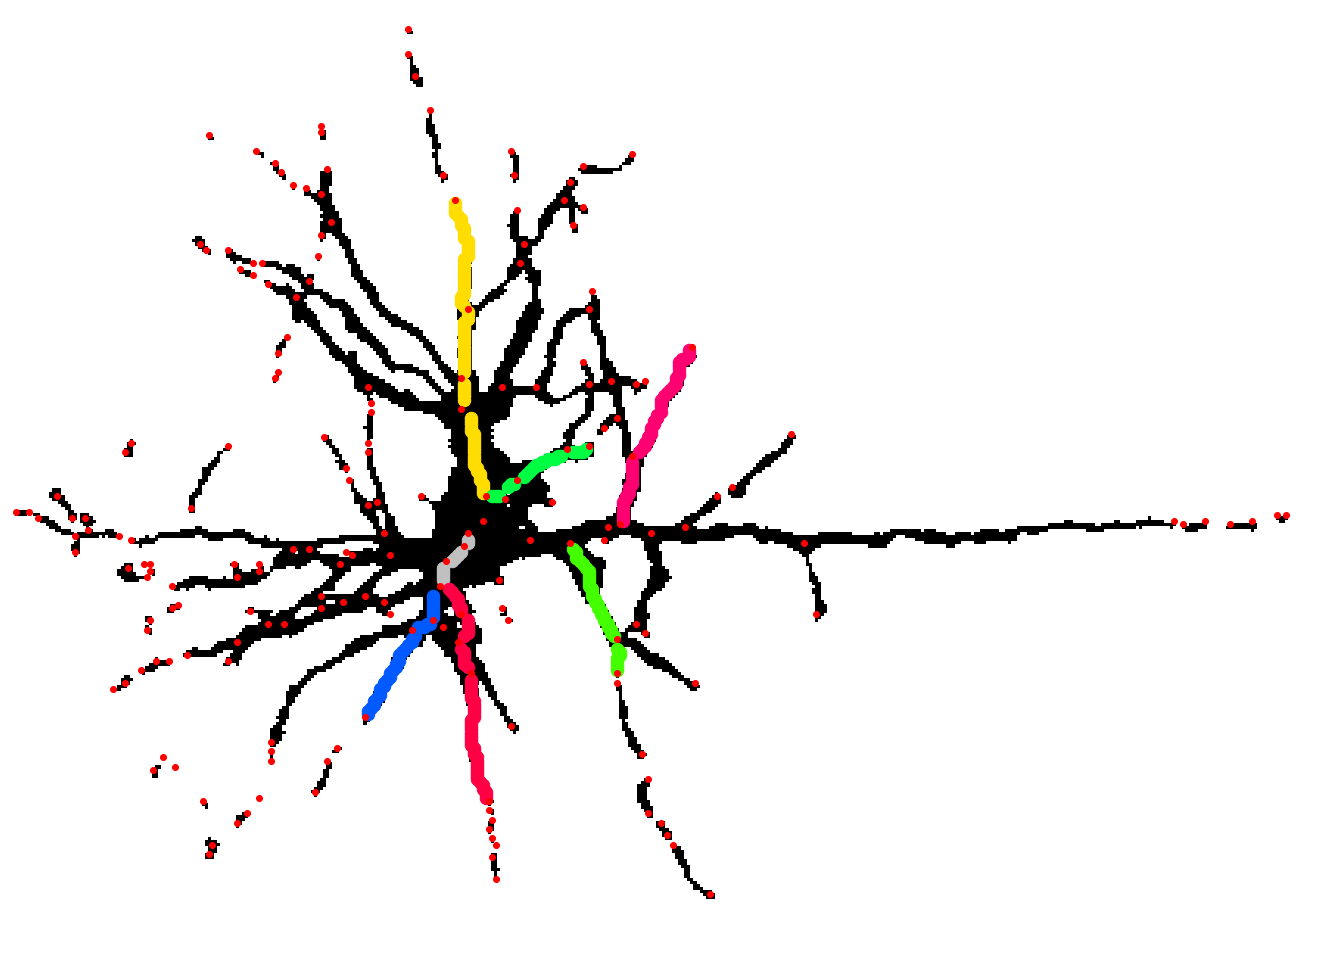
\includegraphics[height=1.5in]{resultImages/Porta10-5b-phil-s10-v056-exactMatch-antLabeled.png}
        \caption{Filamentos correctamente individualizados por el algoritmo propuesto, para la muestra N2 en la Figura \ref{fig:Porta10-5b}, identificados por colores.}
        \label{fig:Porta10Prop}
    \end{subfigure}
    ~ 
    \begin{subfigure}[t]{0.49\textwidth}
        \centering
        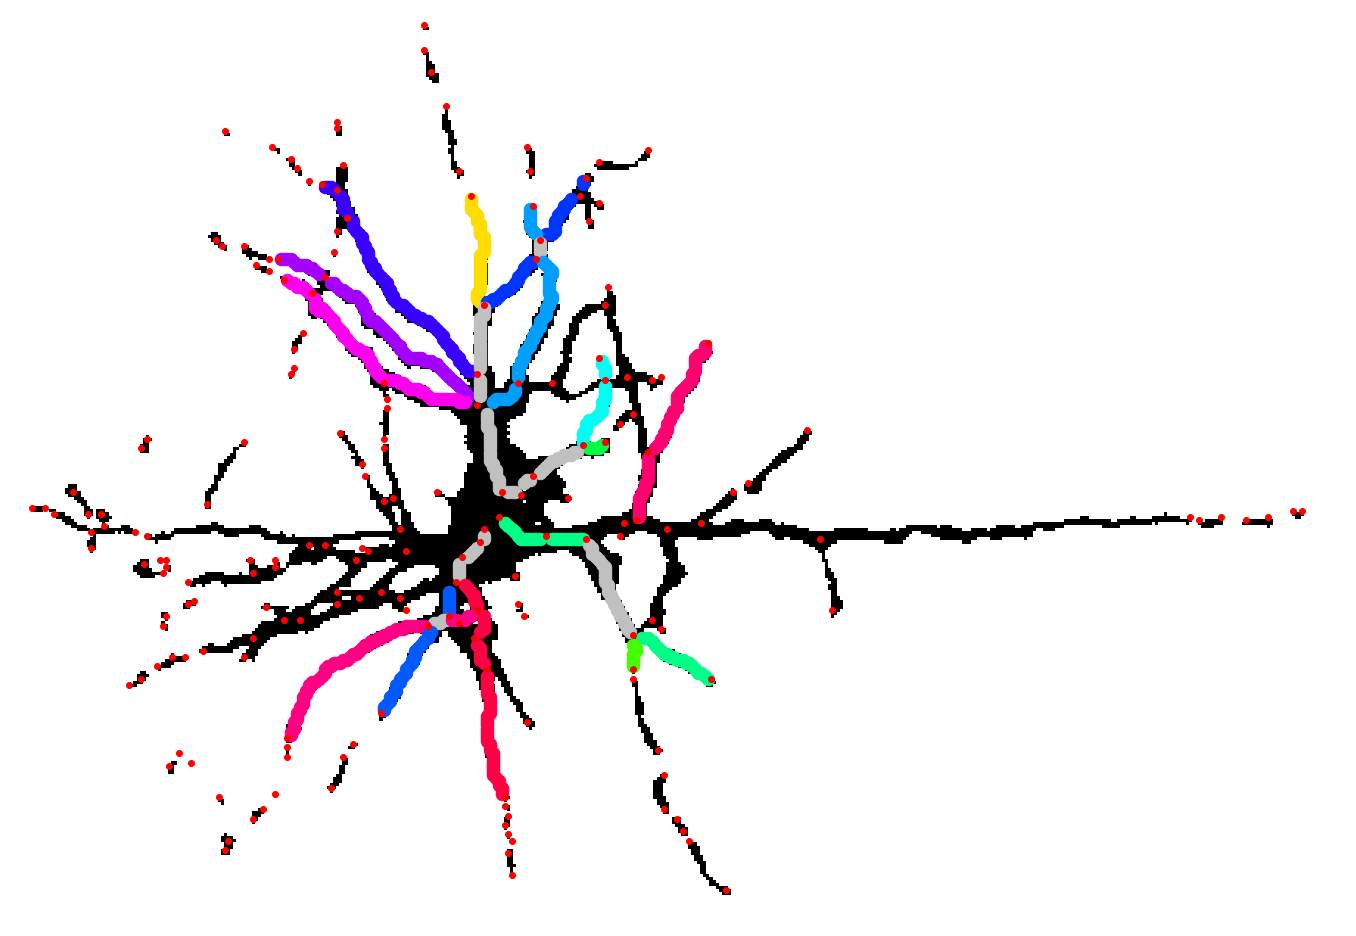
\includegraphics[height=1.5in]{resultImages/Porta10-5b-phil-s10-v056-overmatches-3-antLabeled.png}
        \caption{Filamentos correctamente individualizados en (c) m\'as los filamentos sobre o sub asignados entre 1 a 3 aristas, a partir del resultado del algoritmo propuesto.}
        \label{fig:Port10Best}
    \end{subfigure}
    
    \vskip\baselineskip
    \begin{subfigure}[t]{0.49\textwidth}
        \centering
        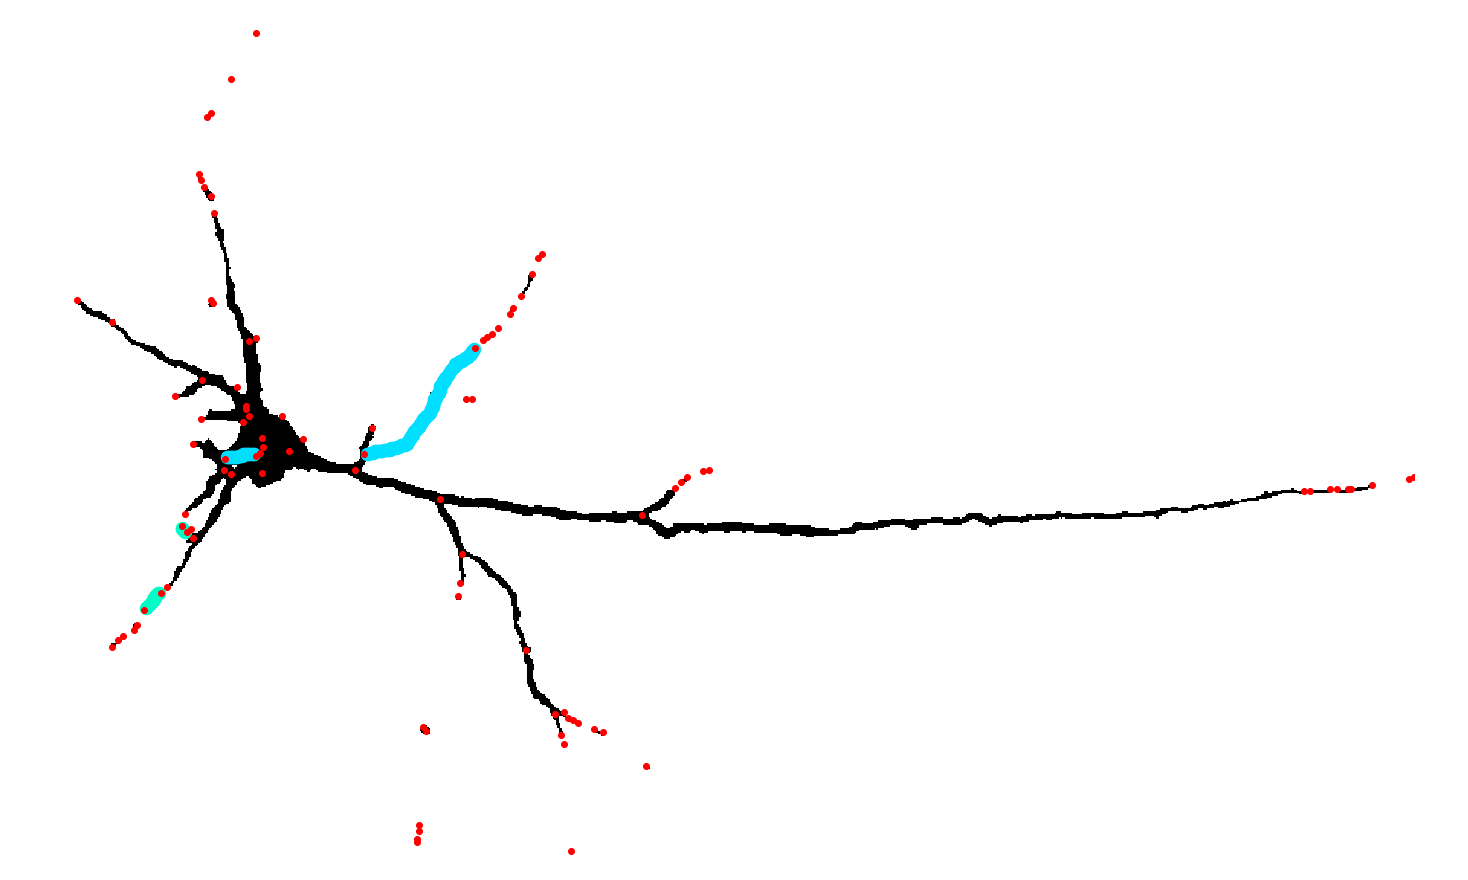
\includegraphics[height=1.5in]{resultImages/Porta18-3a1-phil-s10-v056-exactMatch-antLabeled.png}
        \caption{Filamentos correctamente individualizados por el algoritmo propuesto, para la muestra N3 en la Figura \ref{fig:Porta18-3a1}, identificados por colores.}
        \label{fig:Porta18Prop}
    \end{subfigure}
    ~ 
    \begin{subfigure}[t]{0.49\textwidth}
        \centering
        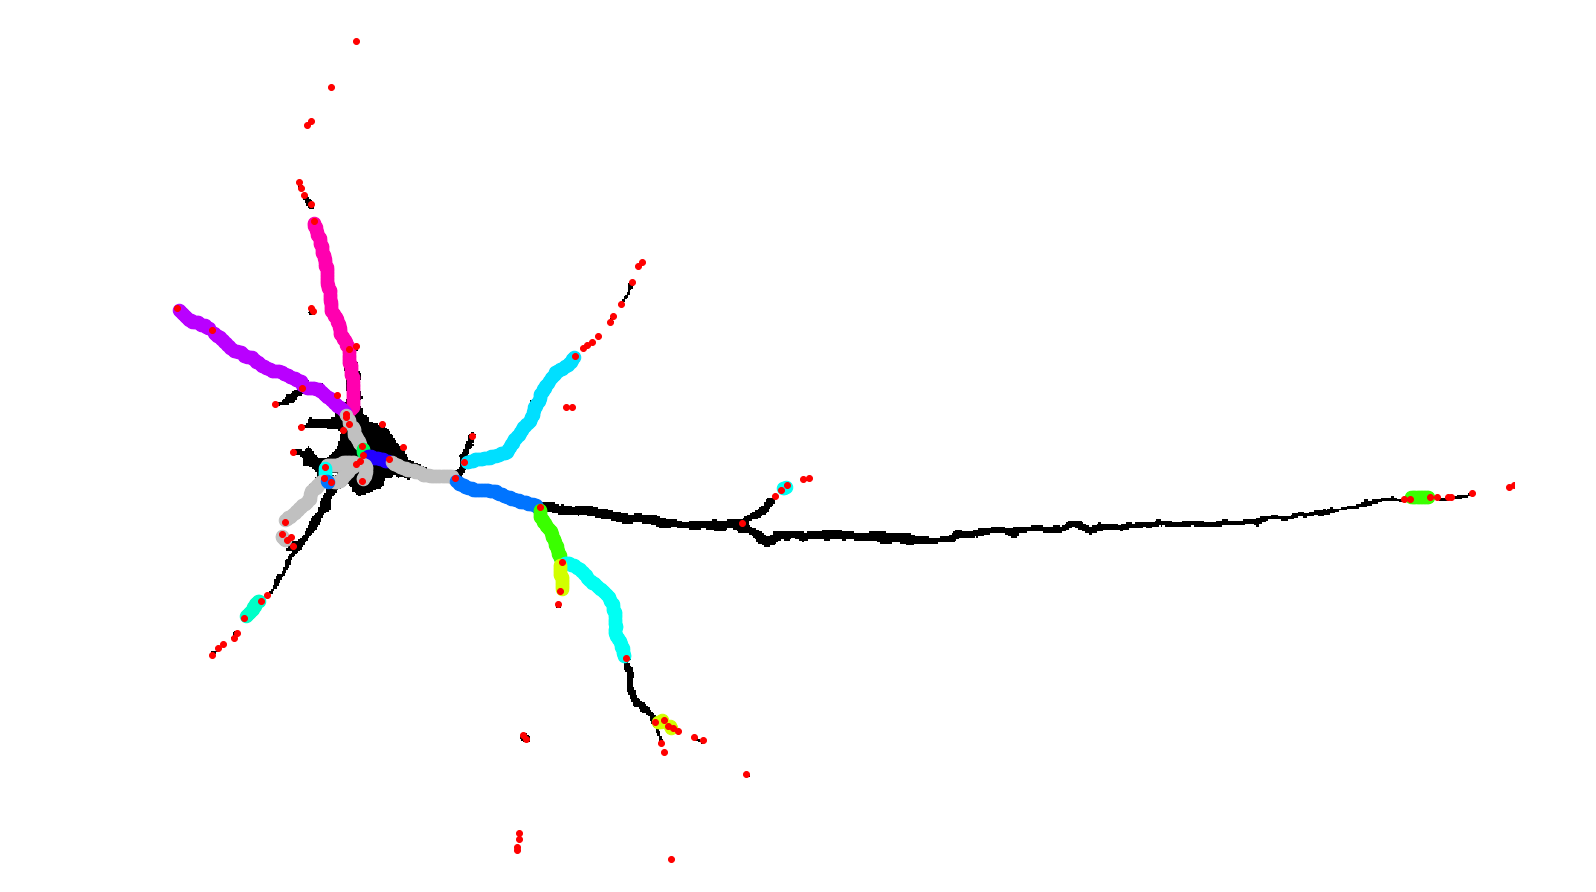
\includegraphics[height=1.5in]{resultImages/Porta18-3a1-phil-s10-v056-overmatches-3-antLabeled.png}
        \caption{Filamentos correctamente individualizados en (e) m\'as los filamentos sobre o sub asignados entre 1 a 3 aristas, a partir del resultado del algoritmo propuesto.}
        \label{fig:Porta18Best}
    \end{subfigure}
    
    \caption{Filamentos propuestos e individualizados correctamente para las muestras N1, N2 y N3, por el algoritmo propuesto. Se puede observar en los filamentos propuestos que existe superposici\'on en las zonas grises, lo que puede identificarse como dendritas que nacen a partir de otras de mayor longitud. Al incluir filamentos sobre o sub asignados en hasta 3 aristas, se puede observar que para las muestras N2 y N3 existen varios filamentos propuestos cerca de ser calces exactos con los definidos por un experto.}% A\'un cuando la individualizaci\'on de calce exacto presenta un n\'umero menor de individualizaciones correctas, es posible ver que las propuestas de filamentos presentan un comportamiento }
    \label{fig:NeuronPropVsCorrect}
\end{figure*}


\section{Resultados Generales}

Observando los resultados obtenidos al individualizar filamentos a partir de im\'agenes sint\'eticas y reales, se tiene que para casos simples existe un comportamiento similar entre el algoritmo propuesto y DeFiNe, con la diferencia de tiempo a favor del algoritmo propuesto. A medida que los filamentos son representados por grafos de mayor complejidad, es decir, con un mayor n\'umero de nodos y aristas, el tiempo de resoluci\'on para el algoritmo propuesto se mantiene en rangos inferiores al minuto, a diferencia de lo que sucede con DeFiNe. La diferencia entre los tiempos de calculo puede ser atribuida parcialmente a la forma en que se explora el espacio de b\'usqueda, teniendo en cuenta la diferencia entre los lenguajes de programaci\'on utilizados para implementar cada m\'etodo. 


Por otra parte, el comportamiento del algoritmo propuesto es estable, tendiendo a individualizar los mismos filamentos en cada iteraci\'on, y pudiendo encontrar filamentos que no aparecen en DeFiNe. Se debe tener en consideraci\'on que el \'ultimo aspecto puede relacionarse con el uso de una ponderaci\'on distinta a la ideal presentada por los autores de DeFiNe, que puede ocasionar la merma en los resultados por aquel m\'etodo. La estabilidad del algoritmo, en conjunto con los par\'ametros predefinidos apunta a favorecer la experiencia del usuario, ya que evita la sintonizaci\'on de par\'ametros, simplificando el trabajo del experto. Adem\'as, la utilizaci\'on de \'ultiples caracter\'isticas en el algoritmo propuesto permite al usuario ajustar par\'ametros espec\'ificos, as\'i como integrar nuevos par\'ametros para manejar informaci\'on adicional que pueda ser incorporada. Otro aspecto que permite mejorar la experiencia del usuario radica en el uso de la curvatura de las aristas, en comparaci\'on a representarlas mediante una l\'inea recta entre 2 nodos. Esto no s\'olo aporta m\'as informaci\'on, sino que adem\'as mejora la visualizaci\'on de los resultados. 

Un an\'alisis particular recae en las m\'etricas y medidas utilizadas para comparar los resultados obtenidos, dado que en el caso de la m\'etrica VI y los \'indices Rand y Jaccard, se pueden obtener resultados que no permiten concluir cual es la calidad del resultado obtenido. Lo anterior se puede observar en la Tabla \ref{tab:VI-R-J-inconclu}, en la que los resultados del \'indice Rand aparecen como de buena calidad, mientras que lo contrario sucede con lo indicado por el \'indice Jaccard. Paralelamente, la m\'etrica VI no refleja correctamente los casos donde hay superposici\'on de filamentos. En base a lo anterior, las otras medidas utilizadas como {\it Precision}, {\it Recall}, y la medida F1 que se deriva de las 2 anteriores, son las que pueden entregar mayor claridad del comportamiento de los m\'etodos probados, ya que permiten observar la individualizaci\'on de filamentos como un problema de clasificaci\'on de aristas en uno o m\'as categor\'ias, siendo cada  categor\'ia un filamento individualizado por un experto.


\begin{table}[h]
\centering
\begin{tabular}{|c|c|c|c|c|c|}
\hline
Figura & Modo/Muestra & VI Max & VI & Rand & Jaccard \\ \hline
 \ref{fig:synth-QFS-7} & 1  & 2.3978 & 1.6360 & 0.7646 & 0.2485 \\
 \ref{fig:synth-QFS-7} & 2  & 2.3978 & 0.7091 & 0.8637 & 0.4750  \\
 \ref{fig:synth-Define-1b} & 3 & 3.0445 & 2.2296 & 0.7276 & 0.1806 \\
 \ref{fig:synth-Define-1b} & 4 & 3.0445 & 2.5878 & 0.7276 & 0.1673  \\
 \ref{fig:SpinningMarchantia} & 5 & 3.4965 & 2.1656 & 0.8658 & 0.2407 \\
 \ref{fig:field3t0filtered1} & 6 & 3.7612 & 2.6285 & 0.8683 & 0.2488  \\
 \ref{fig:field3t0filtered2} & 7 & 1.9459 & 0.4286 & 0.8929 & 0.40 \\
 \ref{fig:Porta6-4a1} & N1 & 6.0258 & 1.7950 & 0.8864 & 0.1389 \\
 \ref{fig:Porta10-5b} & N2 & 5.0814 & 3.7256 & 0.8775 & 0.0703 \\
 \ref{fig:Porta18-3a1} & N3 & 4.2046 & 1.0060 & 0.8794 & 0.2157 \\ \hline
\end{tabular}
\caption{Resultados de la m\'etrica VI y los \'indices Rand y Jaccard para las evaluaciones del algoritmo propuesto en im\'agenes sint\'eticas y reales. Los valores de los \'indices Rand y Jaccard se encuentran en el rango $[0,1]$, siendo 1 el valor ideal. Se observa que los resultados del \'indice Rand se contradicen con los del \'indice Jaccard. Por su parte, la m\'etrica VI penaliza los casos en que una aristas pertenece a m\'as de un filamento propuesto, lo que dificulta la evaluaci\'on mediante esta m\'etrica para los casos de superposici\'on de filamentos.}
\label{tab:VI-R-J-inconclu}
\end{table}

% t-test para cantidad de filamentos propuestos vs gtruth, y correctos vs gtruth
%Para evaluar el desempe\~no general del algoritmo propuesto se calcula la prueba {\it t} de Student o Test-T y la prueba de Kolmog\'orov-Smirnov o prueba K-S sobre los resultados obtenidos por el algoritmo propuesto, DeFiNe, y la individualizaci\'on manual de un experto. En el primer caso se calcula la prueba $t$ de mediciones apareadas independientes, obteni\'endose un {\it p-value} de XXXXX , que al ser mayor que 0.05 no permite rechazar la hip\'otesis nula, por lo que no existe una diferencia estad\'istica significativa entre los resultados del algoritmo propuesto y los de las individualizaciones realizadas por un experto. El resultado de la prueba {\it t} entre el algoritmo propuesto y DeFiNe arroja un resultado similar, con un {\it p-value} de XXXXX, tambi\'en mayor a 0.05, determinando que tampoco existe una diferencia estad\'istica significativa entre los resultados ambos.
%En cuanto a la prueba K-S 


En base a los resultados obtenidos del algoritmo propuesto es posible observar que la relevancia no se encuentra en encontrar una ponderaci\'on entre propiedades o caracter\'isticas para generar mejores resultados, sino en la incorporaci\'on de m\'as caracter\'isticas que permitan reducir el espacio de b\'usqueda y/o descartar soluciones candidatas que no representen el comportamiento biol\'ogico esperado del filamento en la c\'elula observada.
%La flexibilidad que otorga el modelo 

%30\% \'angulo entre aristas, 3,3\% grado de los nodos, 33,3\% posici\'on, 
%16,6\% curvatura, 8,3\% \'angulo entre segmentos y 8,3\% largo de los segmentos
